\documentclass[10pt]{article}
\usepackage[T1]{fontenc}
\usepackage[utf8]{inputenc}
\usepackage[margin=0.62in]{geometry}
\usepackage{amsmath,amssymb}
\usepackage{array,longtable}
\usepackage{graphicx,multicol}
\usepackage{xcolor}
\usepackage{hyperref}
\usepackage{tikz}
\usetikzlibrary{positioning,arrows.meta,calc}
\hypersetup{colorlinks=true,linkcolor=blue!50!black,urlcolor=blue!55!black}
\setlength{\parindent}{0pt}
\setlength{\parskip}{0.45em}
\setlength{\LTpre}{0.2em}
\setlength{\LTpost}{0.6em}
\sloppy
\newcommand{\module}[1]{\texttt{#1}}
\newcommand{\pc}{p_{\mathrm{c}}}
\newcommand{\pt}{\widetilde p}
\newcommand{\prob}{\mathbb P}
\begin{document}

\begin{center}
{\LARGE Sharpness Lean Formalization Inventory}\\[0.35em]
{\large Definitions, theorem statements, and dependency graph}\\[0.35em]
\small Generated from the local Lean sources on 2026-06-25 00:42.
\end{center}
\section*{Proof Completion Check}
\begin{itemize}\item \module{lake env lean Sharpness/Main.lean}: passed.\item \module{lake build}: passed. The emitted messages were style/header linter warnings, not proof errors.\item Source scan over Lean files found no \module{sorry}, \module{axiom}, \module{constant}, \module{unsafe}, \module{admit}, or global \module{set\_option autoImplicit true}.\item \module{\#print axioms Sharpness.sharpness\_zd} returned exactly \(\{\mathrm{propext}, \mathrm{Classical.choice}, \mathrm{Quot.sound}\}\). In particular, no \module{sorryAx} appears.\end{itemize}
The inventory below covers 19 Sharpness modules, 85 definitions/structures/abbreviations, and 283 theorems/lemmas, including 166 private supporting declarations.
\section*{Final Theorem as a Mathematical Statement}

For every dimension \(d \ge 2\), the Lean theorem \module{Sharpness.sharpness\_zd}
proves the conjunction of the following two statements.
\[
\begin{aligned}
&\forall p,\quad 0 \le p < \pc(d)
  \implies \exists c>0,\ \forall n\in\mathbb N,\ 
  \prob_p(0 \leftrightarrow \partial\Lambda_n)
  \le \exp(-c n),\\[0.4em]
&\forall p,\quad \pc(d)<p<1
  \implies
  \theta_d(p)\ge
  \frac{p-\pc(d)}{p(1-\pc(d))}.
\end{aligned}
\]
Here \(\prob_p(0 \leftrightarrow \partial\Lambda_n)\) is formalized as
\module{boxExitProb d p n}; \(\theta_d(p)\) is formalized as
\module{theta d p}; and \(\pc(d)\) is formalized as \module{pCrit d}.

\section*{Core Public Theorems}

\begin{longtable}{>{\raggedright\arraybackslash}p{0.31\textwidth} >{\raggedright\arraybackslash}p{0.62\textwidth}}
\textbf{Lean theorem} & \textbf{Mathematical statement} \\
\hline
\endfirsthead
\textbf{Lean theorem} & \textbf{Mathematical statement} \\
\hline
\endhead
\module{russo\_closed\_pivotal} &
For an increasing finite local event \(E\), \(0<p<1\), the derivative of \(q\mapsto\prob_q(E)\) at \(p\) is
\[
  \frac{1}{1-p}\sum_{e\in\mathrm{supp}(E)}
  \prob_p(e\text{ is closed-pivotal for }E).
\] \\
\module{differential\_inequality} &
For a finite set \(\Lambda\ni0\) and \(0<p<1\),
\[
\frac{d}{dp}\prob_p(0\leftrightarrow \partial\Lambda)
\ge
\frac{\phi_{\min}(p,\Lambda)}{p(1-p)}
\bigl(1-\prob_p(0\leftrightarrow \partial\Lambda)\bigr).
\] \\
\module{ode\_log\_comparison} &
If \(f<1\) on \([q,p]\), \(0<q<p<1\), and
\[
f'(t)\ge \frac{1-f(t)}{t(1-t)}\quad(q<t<p),
\]
then
\[
1-f(p)\le (1-f(q))\frac{q(1-p)}{p(1-q)}.
\] \\
\module{supercritical\_lower\_bound\_above\_pTilde} &
If \(\pt(d)<p<1\), then
\[
\theta_d(p)\ge \frac{p-\pt(d)}{p(1-\pt(d))}.
\] \\
\module{boundary\_inequality} &
For finite \(B,S\subseteq T\), \(u\in S\), and \(B\cap S=\varnothing\),
\[
\prob_p(u\leftrightarrow B\text{ in }T)
\le
\sum_{(x,y)\in\partial S}
p\,\prob_p(u\leftrightarrow x\text{ in }S)\,
\prob_p(y\leftrightarrow B\text{ in }T).
\] \\
\module{exponential\_decay\_below\_pTilde} &
If \(0\le p<\pt(d)\), then there is \(c>0\) such that
\[
\prob_p(0\leftrightarrow \partial\Lambda_n)\le e^{-cn}
\quad\text{for all }n.
\] \\
\module{pTilde\_eq\_pCrit} &
For \(d>0\), the finite-set critical point equals the \(\theta\)-critical point:
\[
\pt(d)=\pc(d).
\] \\
\module{exponential\_decay\_below\_pCrit} &
If \(d>0\) and \(0\le p<\pc(d)\), then finite box exit probabilities decay exponentially. \\
\module{supercritical\_lower\_bound\_above\_pCrit} &
If \(d>0\) and \(\pc(d)<p<1\), then
\[
\theta_d(p)\ge \frac{p-\pc(d)}{p(1-\pc(d))}.
\] \\
\module{sharpness\_zd} &
Combines the two \(\pc(d)\)-form conclusions above for all \(d\ge2\). \\
\end{longtable}

\section*{Important Definitions}

\begin{longtable}{>{\raggedright\arraybackslash}p{0.28\textwidth} >{\raggedright\arraybackslash}p{0.65\textwidth}}
\textbf{Lean definition} & \textbf{Mathematical meaning} \\
\hline
\endfirsthead
\textbf{Lean definition} & \textbf{Mathematical meaning} \\
\hline
\endhead
\module{Vertex d} & The lattice \(\mathbb Z^d\), represented as functions \(\mathrm{Fin}\ d\to\mathbb Z\). \\
\module{Bond d} & An unoriented nearest-neighbor edge, represented by its two endpoint carrier. \\
\module{Config d} & A bond configuration \(\omega:E(\mathbb Z^d)\to\{\mathrm{false},\mathrm{true}\}\). \\
\module{bernProb p A} & The finite Bernoulli product probability of a Boolean event \(A\). \\
\module{LocalEvent d} & A configuration event with an explicit finite bond support. \\
\module{Prob p E} & The probability of a local event \(E\), computed on its finite support. \\
\module{ExitPred Lam omega} & The event that \(0\) connects inside \(\Lambda\) to an open boundary edge leaving \(\Lambda\). \\
\module{exitProb p Lam h0} & The finite-volume exit probability \(\prob_p(0\leftrightarrow\partial\Lambda)\). \\
\module{boxExitProb d p n} & The exit probability from the \(l^1\)-ball \(\Lambda_n\). \\
\module{theta d p} & The infimum over all finite box exit probabilities, i.e. the decreasing-limit proxy. \\
\module{phi p S} & The finite-set criterion quantity \(p\sum_{(x,y)\in\partial S}\prob_p(0\leftrightarrow x\text{ in }S)\). \\
\module{pTilde d} & The supremum of parameters satisfying the finite-set criterion. \\
\module{pCrit d} & The infimum of parameters in \([0,1]\) for which \(\theta_d(p)>0\). \\
\end{longtable}

\section*{Module Dependency Graph}

\begin{center}
\resizebox{\textwidth}{!}{%
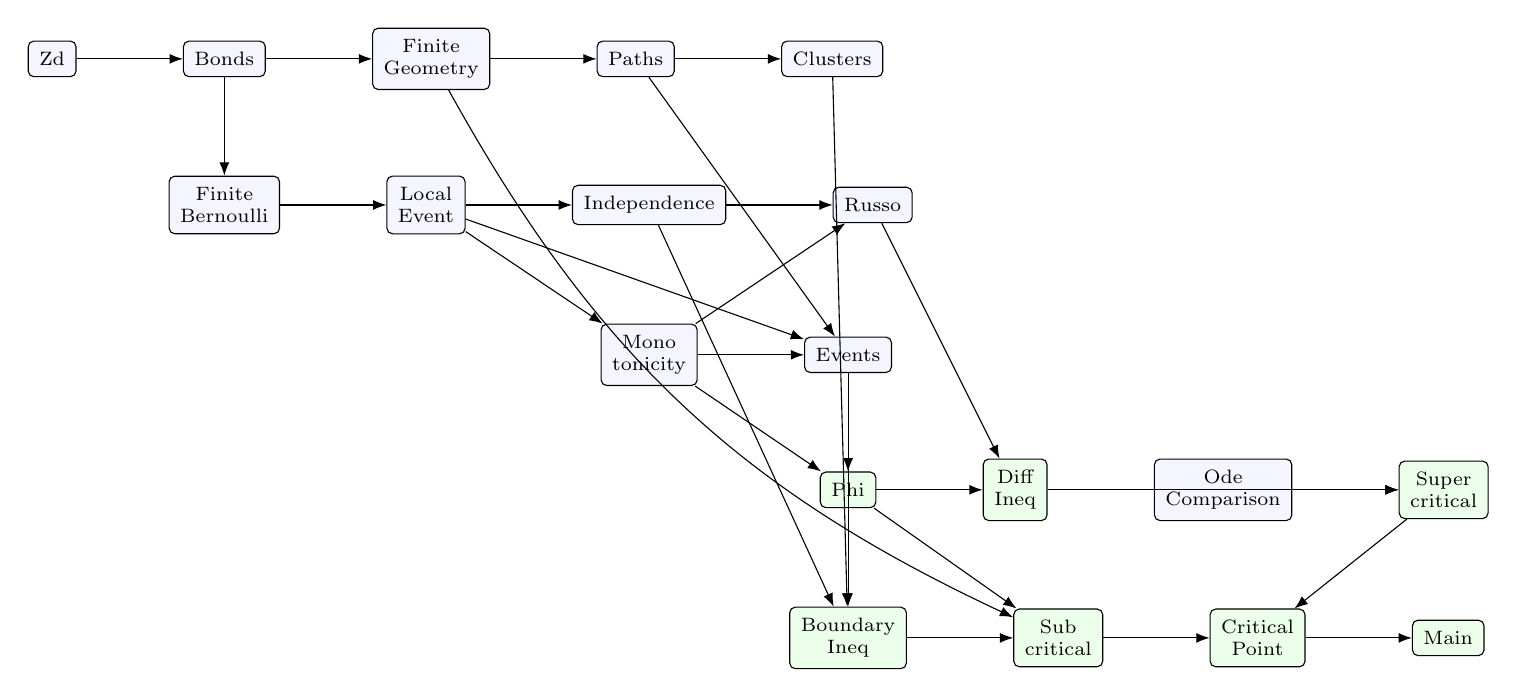
\begin{tikzpicture}[
  node distance=1.25cm and 1.35cm,
  mod/.style={draw, rounded corners=2pt, align=center, font=\scriptsize, fill=blue!4, inner sep=4pt},
  emph/.style={draw, rounded corners=2pt, align=center, font=\scriptsize, fill=green!8, inner sep=4pt},
  arr/.style={-Latex, thin}
]
\node[mod] (Zd) {Zd};
\node[mod, right=of Zd] (Bonds) {Bonds};
\node[mod, right=of Bonds] (FG) {Finite\\Geometry};
\node[mod, right=of FG] (Paths) {Paths};
\node[mod, right=of Paths] (Clusters) {Clusters};

\node[mod, below=of Bonds] (FB) {Finite\\Bernoulli};
\node[mod, right=of FB] (Local) {Local\\Event};
\node[mod, right=of Local] (Indep) {Independence};
\node[mod, below=of Indep] (Mono) {Mono\\tonicity};
\node[mod, right=of Indep] (Russo) {Russo};
\node[mod, right=of Mono] (Events) {Events};

\node[emph, below=of Events] (Phi) {Phi};
\node[emph, right=of Phi] (Diff) {Diff\\Ineq};
\node[mod, right=of Diff] (Ode) {Ode\\Comparison};
\node[emph, right=of Ode] (Super) {Super\\critical};
\node[emph, below=of Phi] (Boundary) {Boundary\\Ineq};
\node[emph, right=of Boundary] (Sub) {Sub\\critical};
\node[emph, right=of Sub] (Crit) {Critical\\Point};
\node[emph, right=of Crit] (Main) {Main};

\draw[arr] (Zd) -- (Bonds);
\draw[arr] (Bonds) -- (FG);
\draw[arr] (FG) -- (Paths);
\draw[arr] (Paths) -- (Clusters);
\draw[arr] (Bonds) -- (FB);
\draw[arr] (FB) -- (Local);
\draw[arr] (Local) -- (Indep);
\draw[arr] (Local) -- (Mono);
\draw[arr] (Indep) -- (Russo);
\draw[arr] (Mono) -- (Russo);
\draw[arr] (Local) -- (Events);
\draw[arr] (Mono) -- (Events);
\draw[arr] (Paths) -- (Events);
\draw[arr] (Events) -- (Phi);
\draw[arr] (Mono) -- (Phi);
\draw[arr] (Phi) -- (Diff);
\draw[arr] (Russo) -- (Diff);
\draw[arr] (Diff) -- (Super);
\draw[arr] (Ode) -- (Super);
\draw[arr] (Clusters) -- (Boundary);
\draw[arr] (Events) -- (Boundary);
\draw[arr] (Indep) -- (Boundary);
\draw[arr] (Boundary) -- (Sub);
\draw[arr] (FG) to[bend right=18] (Sub);
\draw[arr] (Phi) -- (Sub);
\draw[arr] (Sub) -- (Crit);
\draw[arr] (Super) -- (Crit);
\draw[arr] (Crit) -- (Main);
\end{tikzpicture}}
\end{center}

\subsection*{Actual Import Edges}
\begin{multicols}{2}
\begin{itemize}
\item \module{Sharpness.Zd} \(\to\) \module{Sharpness.Bonds}
\item \module{Sharpness.Bonds} \(\to\) \module{Sharpness.FiniteGeometry}
\item \module{Sharpness.FiniteGeometry} \(\to\) \module{Sharpness.Paths}
\item \module{Sharpness.LocalEvent} \(\to\) \module{Sharpness.Clusters}
\item \module{Sharpness.Paths} \(\to\) \module{Sharpness.Clusters}
\item \module{Sharpness.Bonds} \(\to\) \module{Sharpness.FiniteBernoulli}
\item \module{Sharpness.FiniteBernoulli} \(\to\) \module{Sharpness.LocalEvent}
\item \module{Sharpness.LocalEvent} \(\to\) \module{Sharpness.Independence}
\item \module{Sharpness.LocalEvent} \(\to\) \module{Sharpness.Monotonicity}
\item \module{Sharpness.Independence} \(\to\) \module{Sharpness.Russo}
\item \module{Sharpness.Monotonicity} \(\to\) \module{Sharpness.Russo}
\item \module{Sharpness.LocalEvent} \(\to\) \module{Sharpness.Events}
\item \module{Sharpness.Monotonicity} \(\to\) \module{Sharpness.Events}
\item \module{Sharpness.Paths} \(\to\) \module{Sharpness.Events}
\item \module{Sharpness.Events} \(\to\) \module{Sharpness.Phi}
\item \module{Sharpness.Monotonicity} \(\to\) \module{Sharpness.Phi}
\item \module{Sharpness.Phi} \(\to\) \module{Sharpness.DiffIneq}
\item \module{Sharpness.Russo} \(\to\) \module{Sharpness.DiffIneq}
\item \module{Sharpness.DiffIneq} \(\to\) \module{Sharpness.Supercritical}
\item \module{Sharpness.OdeComparison} \(\to\) \module{Sharpness.Supercritical}
\item \module{Sharpness.Clusters} \(\to\) \module{Sharpness.BoundaryIneq}
\item \module{Sharpness.Events} \(\to\) \module{Sharpness.BoundaryIneq}
\item \module{Sharpness.Independence} \(\to\) \module{Sharpness.BoundaryIneq}
\item \module{Sharpness.BoundaryIneq} \(\to\) \module{Sharpness.Subcritical}
\item \module{Sharpness.FiniteGeometry} \(\to\) \module{Sharpness.Subcritical}
\item \module{Sharpness.Phi} \(\to\) \module{Sharpness.Subcritical}
\item \module{Sharpness.Subcritical} \(\to\) \module{Sharpness.CriticalPoint}
\item \module{Sharpness.Supercritical} \(\to\) \module{Sharpness.CriticalPoint}
\item \module{Sharpness.CriticalPoint} \(\to\) \module{Sharpness.Main}
\end{itemize}
\end{multicols}
\section*{Per-File Declaration Inventory}
\subsection*{\module{Sharpness/Zd.lean}}
\textbf{Imports.} \module{Mathlib}.
\paragraph{Definitions, structures, and abbreviations.}
\begin{longtable}{>{\raggedright\arraybackslash}p{0.27\textwidth} >{\raggedright\arraybackslash}p{0.66\textwidth}}
\textbf{Name} & \textbf{Statement or signature} \\
\hline
\endfirsthead
\textbf{Name} & \textbf{Statement or signature} \\
\hline
\endhead
\texttt{Vertex} & {\ttfamily\scriptsize line 8:\allowbreak{} abbrev Vertex (\allowbreak{}d :\allowbreak{} Nat)\allowbreak{} -\allowbreak{}-\allowbreak{} Vertices of nearest-\allowbreak{}neighbor bond percolation on `Z\textasciicircum{}d`.\allowbreak{}} \\[0.45em]
\texttt{l1} & {\ttfamily\scriptsize line 11:\allowbreak{} def l1 \{d :\allowbreak{} Nat\} (\allowbreak{}x :\allowbreak{} Vertex d)\allowbreak{} :\allowbreak{} Nat -\allowbreak{}-\allowbreak{} The `l\textasciicircum{}1` norm on `Z\textasciicircum{}d`,\allowbreak{} valued in `Nat`.\allowbreak{}} \\[0.45em]
\texttt{Adj} & {\ttfamily\scriptsize line 15:\allowbreak{} def Adj \{d :\allowbreak{} Nat\} (\allowbreak{}x y :\allowbreak{} Vertex d)\allowbreak{} :\allowbreak{} Prop -\allowbreak{}-\allowbreak{} Nearest-\allowbreak{}neighbor adjacency on `Z\textasciicircum{}d`.\allowbreak{}} \\[0.45em]
\texttt{translateVertex} & {\ttfamily\scriptsize line 19:\allowbreak{} def translateVertex \{d :\allowbreak{} Nat\} (\allowbreak{}a x :\allowbreak{} Vertex d)\allowbreak{} :\allowbreak{} Vertex d -\allowbreak{}-\allowbreak{} Translate a vertex by another vertex.\allowbreak{}} \\[0.45em]
\texttt{coordStep} & {\ttfamily\scriptsize line 23:\allowbreak{} def coordStep \{d :\allowbreak{} Nat\} (\allowbreak{}i :\allowbreak{} Fin d)\allowbreak{} (\allowbreak{}positive :\allowbreak{} Bool)\allowbreak{} :\allowbreak{} Vertex d -\allowbreak{}-\allowbreak{} A single positive or negative coordinate step.\allowbreak{}} \\[0.45em]
\texttt{coordRange [noncomputable]} & {\ttfamily\scriptsize line 27:\allowbreak{} noncomputable def coordRange (\allowbreak{}n :\allowbreak{} Nat)\allowbreak{} :\allowbreak{} Finset Int -\allowbreak{}-\allowbreak{} Integer coordinates available in the cube containing the `l\textasciicircum{}1` ball.\allowbreak{}} \\[0.45em]
\texttt{cube [noncomputable]} & {\ttfamily\scriptsize line 31:\allowbreak{} noncomputable def cube (\allowbreak{}d n :\allowbreak{} Nat)\allowbreak{} :\allowbreak{} Finset (\allowbreak{}Vertex d)\allowbreak{} -\allowbreak{}-\allowbreak{} The finite coordinate cube `[-\allowbreak{}n,\allowbreak{}n]\textasciicircum{}d`.\allowbreak{}} \\[0.45em]
\texttt{ball [noncomputable]} & {\ttfamily\scriptsize line 41:\allowbreak{} noncomputable def ball (\allowbreak{}d n :\allowbreak{} Nat)\allowbreak{} :\allowbreak{} Finset (\allowbreak{}Vertex d)\allowbreak{} -\allowbreak{}-\allowbreak{} The finite `l\textasciicircum{}1` box `Lambda\_\allowbreak{}n =\allowbreak{} \{x :\allowbreak{} Z\textasciicircum{}d | ||x||\_\allowbreak{}1 <=\allowbreak{} n\}`.\allowbreak{}} \\[0.45em]
\texttt{neighbors [noncomputable]} & {\ttfamily\scriptsize line 45:\allowbreak{} noncomputable def neighbors \{d :\allowbreak{} Nat\} (\allowbreak{}x :\allowbreak{} Vertex d)\allowbreak{} :\allowbreak{} Finset (\allowbreak{}Vertex d)\allowbreak{} -\allowbreak{}-\allowbreak{} The finite set of nearest-\allowbreak{}neighbor candidates of a vertex.\allowbreak{}} \\[0.45em]
\end{longtable}

\paragraph{Theorems and lemmas.}
\begin{longtable}{>{\raggedright\arraybackslash}p{0.27\textwidth} >{\raggedright\arraybackslash}p{0.66\textwidth}}
\textbf{Name} & \textbf{Statement or signature} \\
\hline
\endfirsthead
\textbf{Name} & \textbf{Statement or signature} \\
\hline
\endhead
\texttt{translateVertex\_\allowbreak{}apply} & {\ttfamily\scriptsize line 49:\allowbreak{} theorem translateVertex\_\allowbreak{}apply \{d :\allowbreak{} Nat\} (\allowbreak{}a x :\allowbreak{} Vertex d)\allowbreak{} (\allowbreak{}i :\allowbreak{} Fin d)\allowbreak{} :\allowbreak{} translateVertex a x i =\allowbreak{} x i +\allowbreak{} a i} \\[0.45em]
\texttt{l1\_\allowbreak{}zero} & {\ttfamily\scriptsize line 53:\allowbreak{} theorem l1\_\allowbreak{}zero \{d :\allowbreak{} Nat\} :\allowbreak{} l1 (\allowbreak{}0 :\allowbreak{} Vertex d)\allowbreak{} =\allowbreak{} 0} \\[0.45em]
\texttt{l1\_\allowbreak{}neg} & {\ttfamily\scriptsize line 56:\allowbreak{} theorem l1\_\allowbreak{}neg \{d :\allowbreak{} Nat\} (\allowbreak{}x :\allowbreak{} Vertex d)\allowbreak{} :\allowbreak{} l1 (\allowbreak{}-\allowbreak{}x)\allowbreak{} =\allowbreak{} l1 x} \\[0.45em]
\texttt{l1\_\allowbreak{}add\_\allowbreak{}le} & {\ttfamily\scriptsize line 59:\allowbreak{} theorem l1\_\allowbreak{}add\_\allowbreak{}le \{d :\allowbreak{} Nat\} (\allowbreak{}x y :\allowbreak{} Vertex d)\allowbreak{} :\allowbreak{} l1 (\allowbreak{}x +\allowbreak{} y)\allowbreak{} <=\allowbreak{} l1 x +\allowbreak{} l1 y} \\[0.45em]
\texttt{l1\_\allowbreak{}sub\_\allowbreak{}comm} & {\ttfamily\scriptsize line 72:\allowbreak{} theorem l1\_\allowbreak{}sub\_\allowbreak{}comm \{d :\allowbreak{} Nat\} (\allowbreak{}x y :\allowbreak{} Vertex d)\allowbreak{} :\allowbreak{} l1 (\allowbreak{}x -\allowbreak{} y)\allowbreak{} =\allowbreak{} l1 (\allowbreak{}y -\allowbreak{} x)\allowbreak{}} \\[0.45em]
\texttt{adj\_\allowbreak{}symm} & {\ttfamily\scriptsize line 79:\allowbreak{} theorem adj\_\allowbreak{}symm \{d :\allowbreak{} Nat\} \{x y :\allowbreak{} Vertex d\} (\allowbreak{}hxy :\allowbreak{} Adj x y)\allowbreak{} :\allowbreak{} Adj y x} \\[0.45em]
\texttt{ne\_\allowbreak{}of\_\allowbreak{}adj} & {\ttfamily\scriptsize line 82:\allowbreak{} theorem ne\_\allowbreak{}of\_\allowbreak{}adj \{d :\allowbreak{} Nat\} \{x y :\allowbreak{} Vertex d\} (\allowbreak{}hxy :\allowbreak{} Adj x y)\allowbreak{} :\allowbreak{} x !=\allowbreak{} y} \\[0.45em]
\texttt{mem\_\allowbreak{}cube\_\allowbreak{}iff} & {\ttfamily\scriptsize line 87:\allowbreak{} theorem mem\_\allowbreak{}cube\_\allowbreak{}iff \{d n :\allowbreak{} Nat\} \{x :\allowbreak{} Vertex d\} :\allowbreak{} x in cube d n <-\allowbreak{}> forall i :\allowbreak{} Fin d,\allowbreak{} x i in coordRange n} \\[0.45em]
\texttt{coord\_\allowbreak{}natAbs\_\allowbreak{}le\_\allowbreak{}l1} & {\ttfamily\scriptsize line 103:\allowbreak{} theorem coord\_\allowbreak{}natAbs\_\allowbreak{}le\_\allowbreak{}l1 \{d :\allowbreak{} Nat\} (\allowbreak{}x :\allowbreak{} Vertex d)\allowbreak{} (\allowbreak{}i :\allowbreak{} Fin d)\allowbreak{} :\allowbreak{} Int.\allowbreak{}natAbs (\allowbreak{}x i)\allowbreak{} <=\allowbreak{} l1 x} \\[0.45em]
\texttt{coord\_\allowbreak{}mem\_\allowbreak{}coordRange\_\allowbreak{}of\_\allowbreak{}l1\_\allowbreak{}le} & {\ttfamily\scriptsize line 111:\allowbreak{} theorem coord\_\allowbreak{}mem\_\allowbreak{}coordRange\_\allowbreak{}of\_\allowbreak{}l1\_\allowbreak{}le \{d n :\allowbreak{} Nat\} \{x :\allowbreak{} Vertex d\} (\allowbreak{}hx :\allowbreak{} l1 x <=\allowbreak{} n)\allowbreak{} (\allowbreak{}i :\allowbreak{} Fin d)\allowbreak{} :\allowbreak{} x i in coordRange n} \\[0.45em]
\texttt{mem\_\allowbreak{}ball\_\allowbreak{}iff} & {\ttfamily\scriptsize line 123:\allowbreak{} theorem mem\_\allowbreak{}ball\_\allowbreak{}iff \{d n :\allowbreak{} Nat\} \{x :\allowbreak{} Vertex d\} :\allowbreak{} x in ball d n <-\allowbreak{}> l1 x <=\allowbreak{} n -\allowbreak{}-\allowbreak{} Characterize membership in the finite `l\textasciicircum{}1` ball constructed from the bounded cube.\allowbreak{}} \\[0.45em]
\texttt{zero\_\allowbreak{}mem\_\allowbreak{}ball} & {\ttfamily\scriptsize line 134:\allowbreak{} theorem zero\_\allowbreak{}mem\_\allowbreak{}ball (\allowbreak{}d n :\allowbreak{} Nat)\allowbreak{} :\allowbreak{} (\allowbreak{}0 :\allowbreak{} Vertex d)\allowbreak{} in ball d n -\allowbreak{}-\allowbreak{} The origin belongs to every finite `l\textasciicircum{}1` ball.\allowbreak{}} \\[0.45em]
\texttt{adj\_\allowbreak{}translate\_\allowbreak{}iff} & {\ttfamily\scriptsize line 139:\allowbreak{} theorem adj\_\allowbreak{}translate\_\allowbreak{}iff \{d :\allowbreak{} Nat\} \{a x y :\allowbreak{} Vertex d\} :\allowbreak{} Adj (\allowbreak{}translateVertex a x)\allowbreak{} (\allowbreak{}translateVertex a y)\allowbreak{} <-\allowbreak{}> Adj x y -\allowbreak{}-\allowbreak{} Nearest-\allowbreak{}neighbor adjacency is invariant under translations.\allowbreak{}} \\[0.45em]
\texttt{mem\_\allowbreak{}neighbors\_\allowbreak{}iff} & {\ttfamily\scriptsize line 148:\allowbreak{} theorem mem\_\allowbreak{}neighbors\_\allowbreak{}iff \{d :\allowbreak{} Nat\} \{x y :\allowbreak{} Vertex d\} :\allowbreak{} y in neighbors x <-\allowbreak{}> Adj x y -\allowbreak{}-\allowbreak{} Nearest-\allowbreak{}neighbor candidates are exactly adjacent vertices.\allowbreak{}} \\[0.45em]
\texttt{translate\_\allowbreak{}ball\_\allowbreak{}exit} & {\ttfamily\scriptsize line 170:\allowbreak{} theorem translate\_\allowbreak{}ball\_\allowbreak{}exit \{d n L :\allowbreak{} Nat\} \{y z :\allowbreak{} Vertex d\} (\allowbreak{}hy :\allowbreak{} y in ball d L)\allowbreak{} (\allowbreak{}hz :\allowbreak{} z notin ball d n)\allowbreak{} (\allowbreak{}hLn :\allowbreak{} L <=\allowbreak{} n)\allowbreak{} :\allowbreak{} z -\allowbreak{} y notin ball d (\allowbreak{}n -\allowbreak{} L)\allowbreak{} -\allowbreak{}-\allowbreak{} The triangle estimate used to compare translated exit events.\allowbreak{}} \\[0.45em]
\end{longtable}

\subsection*{\module{Sharpness/Bonds.lean}}
\textbf{Imports.} \module{Sharpness.Zd}.
\paragraph{Definitions, structures, and abbreviations.}
\begin{longtable}{>{\raggedright\arraybackslash}p{0.27\textwidth} >{\raggedright\arraybackslash}p{0.66\textwidth}}
\textbf{Name} & \textbf{Statement or signature} \\
\hline
\endfirsthead
\textbf{Name} & \textbf{Statement or signature} \\
\hline
\endhead
\texttt{Bond} & {\ttfamily\scriptsize line 6:\allowbreak{} structure Bond (\allowbreak{}d :\allowbreak{} Nat)\allowbreak{} -\allowbreak{}-\allowbreak{} An unoriented nearest-\allowbreak{}neighbor bond,\allowbreak{} represented by its two-\allowbreak{}point carrier.\allowbreak{}} \\[0.45em]
\texttt{Config} & {\ttfamily\scriptsize line 13:\allowbreak{} abbrev Config (\allowbreak{}d :\allowbreak{} Nat)\allowbreak{} -\allowbreak{}-\allowbreak{} Global percolation configurations,\allowbreak{} indexed by unoriented bonds.\allowbreak{}} \\[0.45em]
\texttt{bondOfAdj} & {\ttfamily\scriptsize line 33:\allowbreak{} def bondOfAdj \{d :\allowbreak{} Nat\} \{x y :\allowbreak{} Vertex d\} (\allowbreak{}hxy :\allowbreak{} Adj x y)\allowbreak{} :\allowbreak{} Bond d -\allowbreak{}-\allowbreak{} The unoriented bond associated to an adjacent ordered pair.\allowbreak{}} \\[0.45em]
\texttt{OrientedEdge} & {\ttfamily\scriptsize line 39:\allowbreak{} abbrev OrientedEdge (\allowbreak{}d :\allowbreak{} Nat)\allowbreak{} -\allowbreak{}-\allowbreak{} An oriented edge is a pair of vertices.\allowbreak{} Boundary sums use this orientation.\allowbreak{}} \\[0.45em]
\texttt{orientedBoundary [noncomputable]} & {\ttfamily\scriptsize line 42:\allowbreak{} noncomputable def orientedBoundary \{d :\allowbreak{} Nat\} (\allowbreak{}S :\allowbreak{} Finset (\allowbreak{}Vertex d)\allowbreak{})\allowbreak{} :\allowbreak{} Finset (\allowbreak{}OrientedEdge d)\allowbreak{} -\allowbreak{}-\allowbreak{} Oriented boundary edges from a finite vertex set to its complement.\allowbreak{}} \\[0.45em]
\texttt{OEdgeBoundary} & {\ttfamily\scriptsize line 80:\allowbreak{} structure OEdgeBoundary \{d :\allowbreak{} Nat\} (\allowbreak{}S :\allowbreak{} Finset (\allowbreak{}Vertex d)\allowbreak{})\allowbreak{} -\allowbreak{}-\allowbreak{} A boundary edge with its orientation and membership proofs.\allowbreak{}} \\[0.45em]
\texttt{OEdgeBoundary.\allowbreak{}bond} & {\ttfamily\scriptsize line 88:\allowbreak{} def OEdgeBoundary.\allowbreak{}bond \{d :\allowbreak{} Nat\} \{S :\allowbreak{} Finset (\allowbreak{}Vertex d)\allowbreak{}\} (\allowbreak{}e :\allowbreak{} OEdgeBoundary S)\allowbreak{} :\allowbreak{} Bond d -\allowbreak{}-\allowbreak{} Forget the orientation of a boundary edge.\allowbreak{}} \\[0.45em]
\texttt{internalBonds [noncomputable]} & {\ttfamily\scriptsize line 100:\allowbreak{} noncomputable def internalBonds \{d :\allowbreak{} Nat\} (\allowbreak{}S :\allowbreak{} Finset (\allowbreak{}Vertex d)\allowbreak{})\allowbreak{} :\allowbreak{} Finset (\allowbreak{}Bond d)\allowbreak{} -\allowbreak{}-\allowbreak{} Bonds with both endpoints in a finite vertex set.\allowbreak{}} \\[0.45em]
\texttt{exitBonds [noncomputable]} & {\ttfamily\scriptsize line 121:\allowbreak{} noncomputable def exitBonds \{d :\allowbreak{} Nat\} (\allowbreak{}S :\allowbreak{} Finset (\allowbreak{}Vertex d)\allowbreak{})\allowbreak{} :\allowbreak{} Finset (\allowbreak{}Bond d)\allowbreak{} -\allowbreak{}-\allowbreak{} Unoriented bonds crossing the boundary of a finite vertex set.\allowbreak{}} \\[0.45em]
\end{longtable}

\paragraph{Theorems and lemmas.}
\begin{longtable}{>{\raggedright\arraybackslash}p{0.27\textwidth} >{\raggedright\arraybackslash}p{0.66\textwidth}}
\textbf{Name} & \textbf{Statement or signature} \\
\hline
\endfirsthead
\textbf{Name} & \textbf{Statement or signature} \\
\hline
\endhead
\texttt{bondOfAdj\_\allowbreak{}card\_\allowbreak{}two} & {\ttfamily\scriptsize line 16:\allowbreak{} theorem bondOfAdj\_\allowbreak{}card\_\allowbreak{}two \{d :\allowbreak{} Nat\} \{x y :\allowbreak{} Vertex d\} (\allowbreak{}hxy :\allowbreak{} Adj x y)\allowbreak{} :\allowbreak{} (\allowbreak{}\{x,\allowbreak{} y\} :\allowbreak{} Finset (\allowbreak{}Vertex d)\allowbreak{})\allowbreak{}.\allowbreak{}card =\allowbreak{} 2 -\allowbreak{}-\allowbreak{} Adjacent vertices form a two-\allowbreak{}point finite carrier.\allowbreak{}} \\[0.45em]
\texttt{bondOfAdj\_\allowbreak{}adj\_\allowbreak{}pair} & {\ttfamily\scriptsize line 21:\allowbreak{} theorem bondOfAdj\_\allowbreak{}adj\_\allowbreak{}pair \{d :\allowbreak{} Nat\} \{x y :\allowbreak{} Vertex d\} (\allowbreak{}hxy :\allowbreak{} Adj x y)\allowbreak{} :\allowbreak{} forall u,\allowbreak{} u in (\allowbreak{}\{x,\allowbreak{} y\} :\allowbreak{} Finset (\allowbreak{}Vertex d)\allowbreak{})\allowbreak{} -\allowbreak{}> forall v,\allowbreak{} v in (\allowbreak{}\{x,\allowbreak{} y\} :\allowbreak{} Finset (\allowbreak{}Vertex d)\allowbreak{})\allowbreak{} -\allowbreak{}> u !=\allowbreak{} v -\allowbreak{}> Adj u v -\allowbreak{}-\allowbreak{} Every distinct pair in the carrier `\{x,\allowbreak{}y\}` is adjacent when `x` and `y` are adjacent.\allowbreak{}} \\[0.45em]
\texttt{mem\_\allowbreak{}orientedBoundary\_\allowbreak{}iff} & {\ttfamily\scriptsize line 52:\allowbreak{} theorem mem\_\allowbreak{}orientedBoundary\_\allowbreak{}iff \{d :\allowbreak{} Nat\} \{S :\allowbreak{} Finset (\allowbreak{}Vertex d)\allowbreak{}\} \{e :\allowbreak{} OrientedEdge d\} :\allowbreak{} e in orientedBoundary S <-\allowbreak{}> e.\allowbreak{}1 in S /\allowbreak{}\textbackslash{} e.\allowbreak{}2 notin S /\allowbreak{}\textbackslash{} Adj e.\allowbreak{}1 e.\allowbreak{}2 -\allowbreak{}-\allowbreak{} The finite neighbor construction exactly enumerates oriented nearest-\allowbreak{}neighbor boundary edges.\allowbreak{}} \\[0.45em]
\texttt{orientedBoundary\_\allowbreak{}adj} & {\ttfamily\scriptsize line 75:\allowbreak{} theorem orientedBoundary\_\allowbreak{}adj \{d :\allowbreak{} Nat\} \{S :\allowbreak{} Finset (\allowbreak{}Vertex d)\allowbreak{}\} \{e :\allowbreak{} OrientedEdge d\} (\allowbreak{}he :\allowbreak{} e in orientedBoundary S)\allowbreak{} :\allowbreak{} Adj e.\allowbreak{}1 e.\allowbreak{}2 -\allowbreak{}-\allowbreak{} Adjacency proof extracted from membership in the oriented boundary.\allowbreak{}} \\[0.45em]
\texttt{bondOfAdj\_\allowbreak{}same} & {\ttfamily\scriptsize line 91:\allowbreak{} theorem bondOfAdj\_\allowbreak{}same \{d :\allowbreak{} Nat\} \{x y :\allowbreak{} Vertex d\} \{h h' :\allowbreak{} Adj x y\} :\allowbreak{} bondOfAdj h =\allowbreak{} bondOfAdj h'} \\[0.45em]
\texttt{bondOfAdj\_\allowbreak{}symm} & {\ttfamily\scriptsize line 95:\allowbreak{} theorem bondOfAdj\_\allowbreak{}symm \{d :\allowbreak{} Nat\} \{x y :\allowbreak{} Vertex d\} (\allowbreak{}hxy :\allowbreak{} Adj x y)\allowbreak{} :\allowbreak{} bondOfAdj (\allowbreak{}adj\_\allowbreak{}symm hxy)\allowbreak{} =\allowbreak{} bondOfAdj hxy} \\[0.45em]
\texttt{bondOfAdj\_\allowbreak{}mem\_\allowbreak{}internalBonds} & {\ttfamily\scriptsize line 105:\allowbreak{} theorem bondOfAdj\_\allowbreak{}mem\_\allowbreak{}internalBonds \{d :\allowbreak{} Nat\} \{S :\allowbreak{} Finset (\allowbreak{}Vertex d)\allowbreak{}\} \{x y :\allowbreak{} Vertex d\} (\allowbreak{}hx :\allowbreak{} x in S)\allowbreak{} (\allowbreak{}hy :\allowbreak{} y in S)\allowbreak{} (\allowbreak{}hxy :\allowbreak{} Adj x y)\allowbreak{} :\allowbreak{} bondOfAdj hxy in internalBonds S} \\[0.45em]
\texttt{bondOfAdj\_\allowbreak{}mem\_\allowbreak{}exitBonds} & {\ttfamily\scriptsize line 125:\allowbreak{} theorem bondOfAdj\_\allowbreak{}mem\_\allowbreak{}exitBonds \{d :\allowbreak{} Nat\} \{S :\allowbreak{} Finset (\allowbreak{}Vertex d)\allowbreak{}\} \{e :\allowbreak{} OrientedEdge d\} (\allowbreak{}he :\allowbreak{} e in orientedBoundary S)\allowbreak{} :\allowbreak{} bondOfAdj (\allowbreak{}orientedBoundary\_\allowbreak{}adj he)\allowbreak{} in exitBonds S} \\[0.45em]
\texttt{disjoint\_\allowbreak{}internal\_\allowbreak{}exit} & {\ttfamily\scriptsize line 134:\allowbreak{} theorem disjoint\_\allowbreak{}internal\_\allowbreak{}exit \{d :\allowbreak{} Nat\} (\allowbreak{}S :\allowbreak{} Finset (\allowbreak{}Vertex d)\allowbreak{})\allowbreak{} :\allowbreak{} Disjoint (\allowbreak{}internalBonds S)\allowbreak{} (\allowbreak{}exitBonds S)\allowbreak{} -\allowbreak{}-\allowbreak{} Internal and exit bonds of the same finite set are disjoint.\allowbreak{}} \\[0.45em]
\end{longtable}

\subsection*{\module{Sharpness/FiniteGeometry.lean}}
\textbf{Imports.} \module{Sharpness.Bonds}.
\paragraph{Definitions, structures, and abbreviations.}
\begin{longtable}{>{\raggedright\arraybackslash}p{0.27\textwidth} >{\raggedright\arraybackslash}p{0.66\textwidth}}
\textbf{Name} & \textbf{Statement or signature} \\
\hline
\endfirsthead
\textbf{Name} & \textbf{Statement or signature} \\
\hline
\endhead
\texttt{boxInternalBonds [noncomputable]} & {\ttfamily\scriptsize line 6:\allowbreak{} noncomputable def boxInternalBonds (\allowbreak{}d n :\allowbreak{} Nat)\allowbreak{} :\allowbreak{} Finset (\allowbreak{}Bond d)\allowbreak{} -\allowbreak{}-\allowbreak{} Internal bonds of the box `Lambda\_\allowbreak{}n`.\allowbreak{}} \\[0.45em]
\texttt{boxExitBonds [noncomputable]} & {\ttfamily\scriptsize line 10:\allowbreak{} noncomputable def boxExitBonds (\allowbreak{}d n :\allowbreak{} Nat)\allowbreak{} :\allowbreak{} Finset (\allowbreak{}Bond d)\allowbreak{} -\allowbreak{}-\allowbreak{} Exit bonds crossing from `Lambda\_\allowbreak{}n` to its complement.\allowbreak{}} \\[0.45em]
\end{longtable}

\paragraph{Theorems and lemmas.}
\begin{longtable}{>{\raggedright\arraybackslash}p{0.27\textwidth} >{\raggedright\arraybackslash}p{0.66\textwidth}}
\textbf{Name} & \textbf{Statement or signature} \\
\hline
\endfirsthead
\textbf{Name} & \textbf{Statement or signature} \\
\hline
\endhead
\texttt{boundary\_\allowbreak{}endpoint\_\allowbreak{}mem\_\allowbreak{}ball} & {\ttfamily\scriptsize line 18:\allowbreak{} theorem boundary\_\allowbreak{}endpoint\_\allowbreak{}mem\_\allowbreak{}ball \{d L :\allowbreak{} Nat\} \{S :\allowbreak{} Finset (\allowbreak{}Vertex d)\allowbreak{}\} \{e :\allowbreak{} OrientedEdge d\} (\allowbreak{}hL :\allowbreak{} 0 < L)\allowbreak{} (\allowbreak{}hS :\allowbreak{} forall x,\allowbreak{} x in S -\allowbreak{}> x in ball d (\allowbreak{}L -\allowbreak{} 1)\allowbreak{})\allowbreak{} (\allowbreak{}he :\allowbreak{} e in orientedBoundary S)\allowbreak{} :\allowbreak{} e.\allowbreak{}2 in ball d L -\allowbreak{}-\allowbreak{} Boundary endpoints of a finite set contained in `Lambda\_\allowbreak{}(\allowbreak{}L-\allowbreak{}1)\allowbreak{}` lie in `Lambda\_\allowbreak{}L`.\allowbreak{} The positivity hypothesis is needed because `Nat` subtraction saturates:\allowbreak{} at `L =\allowbreak{} 0`,\allowbreak{} `L -\allowbreak{} 1 =\allowbreak{} 0`,\allowbreak{} while a boundary endpoint of `\{0\}` need not be in `Lambda\_\allowbreak{}0`.\allowbreak{}} \\[0.45em]
\end{longtable}

\subsection*{\module{Sharpness/Paths.lean}}
\textbf{Imports.} \module{Sharpness.FiniteGeometry}.
\paragraph{Definitions, structures, and abbreviations.}
\begin{longtable}{>{\raggedright\arraybackslash}p{0.27\textwidth} >{\raggedright\arraybackslash}p{0.66\textwidth}}
\textbf{Name} & \textbf{Statement or signature} \\
\hline
\endfirsthead
\textbf{Name} & \textbf{Statement or signature} \\
\hline
\endhead
\texttt{IsPath} & {\ttfamily\scriptsize line 6:\allowbreak{} def IsPath \{d :\allowbreak{} Nat\} (\allowbreak{}gamma :\allowbreak{} List (\allowbreak{}Vertex d)\allowbreak{})\allowbreak{} :\allowbreak{} Prop -\allowbreak{}-\allowbreak{} A list of vertices with adjacent consecutive entries.\allowbreak{}} \\[0.45em]
\texttt{PathFromTo} & {\ttfamily\scriptsize line 10:\allowbreak{} def PathFromTo \{d :\allowbreak{} Nat\} (\allowbreak{}gamma :\allowbreak{} List (\allowbreak{}Vertex d)\allowbreak{})\allowbreak{} (\allowbreak{}x y :\allowbreak{} Vertex d)\allowbreak{} :\allowbreak{} Prop -\allowbreak{}-\allowbreak{} A path from `x` to `y`,\allowbreak{} represented as a finite list.\allowbreak{}} \\[0.45em]
\texttt{PathIn} & {\ttfamily\scriptsize line 14:\allowbreak{} def PathIn \{d :\allowbreak{} Nat\} (\allowbreak{}S :\allowbreak{} Finset (\allowbreak{}Vertex d)\allowbreak{})\allowbreak{} (\allowbreak{}gamma :\allowbreak{} List (\allowbreak{}Vertex d)\allowbreak{})\allowbreak{} :\allowbreak{} Prop -\allowbreak{}-\allowbreak{} Every vertex of the path lies in the finite set `S`.\allowbreak{}} \\[0.45em]
\texttt{OpenPath} & {\ttfamily\scriptsize line 18:\allowbreak{} def OpenPath \{d :\allowbreak{} Nat\} (\allowbreak{}omega :\allowbreak{} Config d)\allowbreak{} (\allowbreak{}gamma :\allowbreak{} List (\allowbreak{}Vertex d)\allowbreak{})\allowbreak{} :\allowbreak{} Prop -\allowbreak{}-\allowbreak{} Every consecutive bond of the path is open in the configuration.\allowbreak{}} \\[0.45em]
\texttt{ConnIn} & {\ttfamily\scriptsize line 22:\allowbreak{} def ConnIn \{d :\allowbreak{} Nat\} (\allowbreak{}omega :\allowbreak{} Config d)\allowbreak{} (\allowbreak{}S :\allowbreak{} Finset (\allowbreak{}Vertex d)\allowbreak{})\allowbreak{} (\allowbreak{}x y :\allowbreak{} Vertex d)\allowbreak{} :\allowbreak{} Prop -\allowbreak{}-\allowbreak{} Open connectivity inside a finite vertex set.\allowbreak{}} \\[0.45em]
\end{longtable}

\paragraph{Theorems and lemmas.}
\begin{longtable}{>{\raggedright\arraybackslash}p{0.27\textwidth} >{\raggedright\arraybackslash}p{0.66\textwidth}}
\textbf{Name} & \textbf{Statement or signature} \\
\hline
\endfirsthead
\textbf{Name} & \textbf{Statement or signature} \\
\hline
\endhead
\texttt{first\_\allowbreak{}exit\_\allowbreak{}step\_\allowbreak{}of\_\allowbreak{}path} & {\ttfamily\scriptsize line 28:\allowbreak{} theorem first\_\allowbreak{}exit\_\allowbreak{}step\_\allowbreak{}of\_\allowbreak{}path \{d :\allowbreak{} Nat\} \{S :\allowbreak{} Finset (\allowbreak{}Vertex d)\allowbreak{}\} \{gamma :\allowbreak{} List (\allowbreak{}Vertex d)\allowbreak{}\} \{x y :\allowbreak{} Vertex d\} (\allowbreak{}hgamma :\allowbreak{} PathFromTo gamma x y)\allowbreak{} (\allowbreak{}hx :\allowbreak{} x in S)\allowbreak{} (\allowbreak{}hy :\allowbreak{} y notin S)\allowbreak{} :\allowbreak{} exists u v :\allowbreak{} Vertex d,\allowbreak{} u in gamma /\allowbreak{}\textbackslash{} v in gamma /\allowbreak{}\textbackslash{} Adj u v /\allowbreak{}\textbackslash{} u in S /\allowbreak{}\textbackslash{} v notin S -\allowbreak{}-\allowbreak{} A path that starts in `S` and ends outside `S` has a crossing step.\allowbreak{}} \\[0.45em]
\texttt{last\_\allowbreak{}exit\_\allowbreak{}step\_\allowbreak{}of\_\allowbreak{}path} & {\ttfamily\scriptsize line 62:\allowbreak{} theorem last\_\allowbreak{}exit\_\allowbreak{}step\_\allowbreak{}of\_\allowbreak{}path \{d :\allowbreak{} Nat\} \{S :\allowbreak{} Finset (\allowbreak{}Vertex d)\allowbreak{}\} \{gamma :\allowbreak{} List (\allowbreak{}Vertex d)\allowbreak{}\} \{x y :\allowbreak{} Vertex d\} (\allowbreak{}hgamma :\allowbreak{} PathFromTo gamma x y)\allowbreak{} (\allowbreak{}hx :\allowbreak{} x in S)\allowbreak{} (\allowbreak{}hy :\allowbreak{} y notin S)\allowbreak{} :\allowbreak{} exists u v :\allowbreak{} Vertex d,\allowbreak{} u in gamma /\allowbreak{}\textbackslash{} v in gamma /\allowbreak{}\textbackslash{} Adj u v /\allowbreak{}\textbackslash{} u in S /\allowbreak{}\textbackslash{} v notin S -\allowbreak{}-\allowbreak{} A path crossing from `S` to its complement has a boundary step; this alias is used for last-\allowbreak{}exit arguments before the later proof refines the chosen crossing.\allowbreak{}} \\[0.45em]
\texttt{isPath\_\allowbreak{}reverse} & {\ttfamily\scriptsize line 69:\allowbreak{} theorem isPath\_\allowbreak{}reverse \{d :\allowbreak{} Nat\} \{gamma :\allowbreak{} List (\allowbreak{}Vertex d)\allowbreak{}\} (\allowbreak{}hgamma :\allowbreak{} IsPath gamma)\allowbreak{} :\allowbreak{} IsPath gamma.\allowbreak{}reverse} \\[0.45em]
\texttt{pathFromTo\_\allowbreak{}reverse} & {\ttfamily\scriptsize line 74:\allowbreak{} theorem pathFromTo\_\allowbreak{}reverse \{d :\allowbreak{} Nat\} \{gamma :\allowbreak{} List (\allowbreak{}Vertex d)\allowbreak{}\} \{x y :\allowbreak{} Vertex d\} (\allowbreak{}hgamma :\allowbreak{} PathFromTo gamma x y)\allowbreak{} :\allowbreak{} PathFromTo gamma.\allowbreak{}reverse y x} \\[0.45em]
\texttt{pathIn\_\allowbreak{}reverse} & {\ttfamily\scriptsize line 82:\allowbreak{} theorem pathIn\_\allowbreak{}reverse \{d :\allowbreak{} Nat\} \{S :\allowbreak{} Finset (\allowbreak{}Vertex d)\allowbreak{}\} \{gamma :\allowbreak{} List (\allowbreak{}Vertex d)\allowbreak{}\} (\allowbreak{}hgamma :\allowbreak{} PathIn S gamma)\allowbreak{} :\allowbreak{} PathIn S gamma.\allowbreak{}reverse} \\[0.45em]
\texttt{openPath\_\allowbreak{}reverse} & {\ttfamily\scriptsize line 87:\allowbreak{} theorem openPath\_\allowbreak{}reverse \{d :\allowbreak{} Nat\} \{omega :\allowbreak{} Config d\} \{gamma :\allowbreak{} List (\allowbreak{}Vertex d)\allowbreak{}\} (\allowbreak{}hgamma :\allowbreak{} OpenPath omega gamma)\allowbreak{} :\allowbreak{} OpenPath omega gamma.\allowbreak{}reverse} \\[0.45em]
\texttt{connIn\_\allowbreak{}symm} & {\ttfamily\scriptsize line 95:\allowbreak{} theorem connIn\_\allowbreak{}symm \{d :\allowbreak{} Nat\} \{omega :\allowbreak{} Config d\} \{S :\allowbreak{} Finset (\allowbreak{}Vertex d)\allowbreak{}\} \{x y :\allowbreak{} Vertex d\} (\allowbreak{}hxy :\allowbreak{} ConnIn omega S x y)\allowbreak{} :\allowbreak{} ConnIn omega S y x -\allowbreak{}-\allowbreak{} Reversing a path preserves open connectivity.\allowbreak{}} \\[0.45em]
\texttt{isPath\_\allowbreak{}translate} & {\ttfamily\scriptsize line 101:\allowbreak{} theorem isPath\_\allowbreak{}translate \{d :\allowbreak{} Nat\} \{a :\allowbreak{} Vertex d\} \{gamma :\allowbreak{} List (\allowbreak{}Vertex d)\allowbreak{}\} (\allowbreak{}hgamma :\allowbreak{} IsPath gamma)\allowbreak{} :\allowbreak{} IsPath (\allowbreak{}gamma.\allowbreak{}map (\allowbreak{}translateVertex a)\allowbreak{})\allowbreak{}} \\[0.45em]
\texttt{pathFromTo\_\allowbreak{}translate} & {\ttfamily\scriptsize line 106:\allowbreak{} theorem pathFromTo\_\allowbreak{}translate \{d :\allowbreak{} Nat\} \{a x y :\allowbreak{} Vertex d\} \{gamma :\allowbreak{} List (\allowbreak{}Vertex d)\allowbreak{}\} (\allowbreak{}hgamma :\allowbreak{} PathFromTo gamma x y)\allowbreak{} :\allowbreak{} PathFromTo (\allowbreak{}gamma.\allowbreak{}map (\allowbreak{}translateVertex a)\allowbreak{})\allowbreak{} (\allowbreak{}translateVertex a x)\allowbreak{} (\allowbreak{}translateVertex a y)\allowbreak{}} \\[0.45em]
\texttt{pathIn\_\allowbreak{}translate} & {\ttfamily\scriptsize line 113:\allowbreak{} theorem pathIn\_\allowbreak{}translate \{d :\allowbreak{} Nat\} \{a :\allowbreak{} Vertex d\} \{S :\allowbreak{} Finset (\allowbreak{}Vertex d)\allowbreak{}\} \{gamma :\allowbreak{} List (\allowbreak{}Vertex d)\allowbreak{}\} (\allowbreak{}hgamma :\allowbreak{} PathIn S gamma)\allowbreak{} :\allowbreak{} PathIn (\allowbreak{}S.\allowbreak{}image (\allowbreak{}translateVertex a)\allowbreak{})\allowbreak{} (\allowbreak{}gamma.\allowbreak{}map (\allowbreak{}translateVertex a)\allowbreak{})\allowbreak{}} \\[0.45em]
\texttt{openPath\_\allowbreak{}translate\_\allowbreak{}of\_\allowbreak{}edge\_\allowbreak{}open} & {\ttfamily\scriptsize line 121:\allowbreak{} theorem openPath\_\allowbreak{}translate\_\allowbreak{}of\_\allowbreak{}edge\_\allowbreak{}open \{d :\allowbreak{} Nat\} \{omega :\allowbreak{} Config d\} \{a :\allowbreak{} Vertex d\} \{gamma :\allowbreak{} List (\allowbreak{}Vertex d)\allowbreak{}\} (\allowbreak{}hopen\_\allowbreak{}translate :\allowbreak{} forall \{u v :\allowbreak{} Vertex d\} (\allowbreak{}huv :\allowbreak{} Adj u v)\allowbreak{},\allowbreak{} omega (\allowbreak{}bondOfAdj huv)\allowbreak{} =\allowbreak{} true -\allowbreak{}> omega (\allowbreak{}bondOfAdj (\allowbreak{}(\allowbreak{}adj\_\allowbreak{}translate\_\allowbreak{}iff (\allowbreak{}a} \\[0.45em]
\texttt{connIn\_\allowbreak{}translate} & {\ttfamily\scriptsize line 134:\allowbreak{} theorem connIn\_\allowbreak{}translate \{d :\allowbreak{} Nat\} \{omega :\allowbreak{} Config d\} \{S :\allowbreak{} Finset (\allowbreak{}Vertex d)\allowbreak{}\} \{a x y :\allowbreak{} Vertex d\} (\allowbreak{}hopen\_\allowbreak{}translate :\allowbreak{} forall \{u v :\allowbreak{} Vertex d\} (\allowbreak{}huv :\allowbreak{} Adj u v)\allowbreak{},\allowbreak{} omega (\allowbreak{}bondOfAdj huv)\allowbreak{} =\allowbreak{} true -\allowbreak{}> omega (\allowbreak{}bondOfAdj (\allowbreak{}(\allowbreak{}adj\_\allowbreak{}translate\_\allowbreak{}iff (\allowbreak{}a -\allowbreak{}-\allowbreak{} Translated paths preserve open connectivity when translated open edges remain open.\allowbreak{}} \\[0.45em]
\end{longtable}

\subsection*{\module{Sharpness/Clusters.lean}}
\textbf{Imports.} \module{Sharpness.LocalEvent}, \module{Sharpness.Paths}.
\paragraph{Definitions, structures, and abbreviations.}
\begin{longtable}{>{\raggedright\arraybackslash}p{0.27\textwidth} >{\raggedright\arraybackslash}p{0.66\textwidth}}
\textbf{Name} & \textbf{Statement or signature} \\
\hline
\endfirsthead
\textbf{Name} & \textbf{Statement or signature} \\
\hline
\endhead
\texttt{clusterIn [noncomputable]} & {\ttfamily\scriptsize line 7:\allowbreak{} noncomputable def clusterIn \{d :\allowbreak{} Nat\} (\allowbreak{}omega :\allowbreak{} Config d)\allowbreak{} (\allowbreak{}S :\allowbreak{} Finset (\allowbreak{}Vertex d)\allowbreak{})\allowbreak{} (\allowbreak{}u :\allowbreak{} Vertex d)\allowbreak{} :\allowbreak{} Finset (\allowbreak{}Vertex d)\allowbreak{} -\allowbreak{}-\allowbreak{} The open cluster of `u` inside a finite vertex set `S`.\allowbreak{}} \\[0.45em]
\texttt{ClusterEqPred} & {\ttfamily\scriptsize line 13:\allowbreak{} def ClusterEqPred \{d :\allowbreak{} Nat\} (\allowbreak{}S C :\allowbreak{} Finset (\allowbreak{}Vertex d)\allowbreak{})\allowbreak{} (\allowbreak{}u :\allowbreak{} Vertex d)\allowbreak{} (\allowbreak{}omega :\allowbreak{} Config d)\allowbreak{} :\allowbreak{} Prop -\allowbreak{}-\allowbreak{} Predicate that the finite cluster inside `S` is exactly `C`.\allowbreak{}} \\[0.45em]
\texttt{clusterIncidentBonds [noncomputable]} & {\ttfamily\scriptsize line 18:\allowbreak{} noncomputable def clusterIncidentBonds \{d :\allowbreak{} Nat\} (\allowbreak{}S C :\allowbreak{} Finset (\allowbreak{}Vertex d)\allowbreak{})\allowbreak{} :\allowbreak{} Finset (\allowbreak{}Bond d)\allowbreak{} -\allowbreak{}-\allowbreak{} Bonds inside `S` with at least one endpoint in the candidate cluster `C`.\allowbreak{}} \\[0.45em]
\end{longtable}

\paragraph{Theorems and lemmas.}
\begin{longtable}{>{\raggedright\arraybackslash}p{0.27\textwidth} >{\raggedright\arraybackslash}p{0.66\textwidth}}
\textbf{Name} & \textbf{Statement or signature} \\
\hline
\endfirsthead
\textbf{Name} & \textbf{Statement or signature} \\
\hline
\endhead
\texttt{bondOfAdj\_\allowbreak{}mem\_\allowbreak{}clusterIncidentBonds [private]} & {\ttfamily\scriptsize line 25:\allowbreak{} private theorem bondOfAdj\_\allowbreak{}mem\_\allowbreak{}clusterIncidentBonds \{d :\allowbreak{} Nat\} \{S C :\allowbreak{} Finset (\allowbreak{}Vertex d)\allowbreak{}\} \{x y :\allowbreak{} Vertex d\} (\allowbreak{}hxS :\allowbreak{} x in S)\allowbreak{} (\allowbreak{}hyS :\allowbreak{} y in S)\allowbreak{} (\allowbreak{}hxy :\allowbreak{} Adj x y)\allowbreak{} (\allowbreak{}hinc :\allowbreak{} x in C \textbackslash{}/\allowbreak{} y in C)\allowbreak{} :\allowbreak{} bondOfAdj hxy in clusterIncidentBonds S C} \\[0.45em]
\texttt{connIn\_\allowbreak{}single [private]} & {\ttfamily\scriptsize line 42:\allowbreak{} private theorem connIn\_\allowbreak{}single \{d :\allowbreak{} Nat\} \{omega :\allowbreak{} Config d\} \{S :\allowbreak{} Finset (\allowbreak{}Vertex d)\allowbreak{}\} \{x :\allowbreak{} Vertex d\} (\allowbreak{}hx :\allowbreak{} x in S)\allowbreak{} :\allowbreak{} ConnIn omega S x x} \\[0.45em]
\texttt{connIn\_\allowbreak{}append\_\allowbreak{}open\_\allowbreak{}adj\_\allowbreak{}same [private]} & {\ttfamily\scriptsize line 51:\allowbreak{} private theorem connIn\_\allowbreak{}append\_\allowbreak{}open\_\allowbreak{}adj\_\allowbreak{}same \{d :\allowbreak{} Nat\} \{omega :\allowbreak{} Config d\} \{S :\allowbreak{} Finset (\allowbreak{}Vertex d)\allowbreak{}\} \{x y z :\allowbreak{} Vertex d\} (\allowbreak{}hzS :\allowbreak{} z in S)\allowbreak{} (\allowbreak{}hyz :\allowbreak{} Adj y z)\allowbreak{} (\allowbreak{}hopen :\allowbreak{} omega (\allowbreak{}bondOfAdj hyz)\allowbreak{} =\allowbreak{} true)\allowbreak{} (\allowbreak{}hconn :\allowbreak{} ConnIn omega S x y)\allowbreak{} :\allowbreak{} ConnIn omega S x z} \\[0.45em]
\texttt{mem\_\allowbreak{}cluster\_\allowbreak{}of\_\allowbreak{}conn [private]} & {\ttfamily\scriptsize line 88:\allowbreak{} private theorem mem\_\allowbreak{}cluster\_\allowbreak{}of\_\allowbreak{}conn \{d :\allowbreak{} Nat\} \{omega :\allowbreak{} Config d\} \{S C :\allowbreak{} Finset (\allowbreak{}Vertex d)\allowbreak{}\} \{u x :\allowbreak{} Vertex d\} (\allowbreak{}hC :\allowbreak{} clusterIn omega S u =\allowbreak{} C)\allowbreak{} (\allowbreak{}hconn :\allowbreak{} ConnIn omega S u x)\allowbreak{} :\allowbreak{} x in C} \\[0.45em]
\texttt{conn\_\allowbreak{}of\_\allowbreak{}mem\_\allowbreak{}cluster [private]} & {\ttfamily\scriptsize line 99:\allowbreak{} private theorem conn\_\allowbreak{}of\_\allowbreak{}mem\_\allowbreak{}cluster \{d :\allowbreak{} Nat\} \{omega :\allowbreak{} Config d\} \{S C :\allowbreak{} Finset (\allowbreak{}Vertex d)\allowbreak{}\} \{u x :\allowbreak{} Vertex d\} (\allowbreak{}hC :\allowbreak{} clusterIn omega S u =\allowbreak{} C)\allowbreak{} (\allowbreak{}hxC :\allowbreak{} x in C)\allowbreak{} :\allowbreak{} ConnIn omega S u x} \\[0.45em]
\texttt{target\_\allowbreak{}mem\_\allowbreak{}of\_\allowbreak{}connIn [private]} & {\ttfamily\scriptsize line 107:\allowbreak{} private theorem target\_\allowbreak{}mem\_\allowbreak{}of\_\allowbreak{}connIn \{d :\allowbreak{} Nat\} \{omega :\allowbreak{} Config d\} \{S :\allowbreak{} Finset (\allowbreak{}Vertex d)\allowbreak{}\} \{u x :\allowbreak{} Vertex d\} (\allowbreak{}hconn :\allowbreak{} ConnIn omega S u x)\allowbreak{} :\allowbreak{} x in S} \\[0.45em]
\texttt{mem\_\allowbreak{}clusterIn\_\allowbreak{}of\_\allowbreak{}conn [private]} & {\ttfamily\scriptsize line 113:\allowbreak{} private theorem mem\_\allowbreak{}clusterIn\_\allowbreak{}of\_\allowbreak{}conn \{d :\allowbreak{} Nat\} \{omega :\allowbreak{} Config d\} \{S :\allowbreak{} Finset (\allowbreak{}Vertex d)\allowbreak{}\} \{u x :\allowbreak{} Vertex d\} (\allowbreak{}hconn :\allowbreak{} ConnIn omega S u x)\allowbreak{} :\allowbreak{} x in clusterIn omega S u} \\[0.45em]
\texttt{openPath\_\allowbreak{}transfer\_\allowbreak{}from\_\allowbreak{}cluster\_\allowbreak{}eq [private]} & {\ttfamily\scriptsize line 119:\allowbreak{} private theorem openPath\_\allowbreak{}transfer\_\allowbreak{}from\_\allowbreak{}cluster\_\allowbreak{}eq \{d :\allowbreak{} Nat\} \{omega omega' :\allowbreak{} Config d\} \{S C :\allowbreak{} Finset (\allowbreak{}Vertex d)\allowbreak{}\} \{u :\allowbreak{} Vertex d\} (\allowbreak{}hsame :\allowbreak{} forall e,\allowbreak{} e in clusterIncidentBonds S C -\allowbreak{}> omega e =\allowbreak{} omega' e)\allowbreak{} (\allowbreak{}hC :\allowbreak{} clusterIn omega S u =\allowbreak{} C)\allowbreak{} \{gamma :\allowbreak{} List (\allowbreak{}Vertex d)\allowbreak{}\} (\allowbreak{}hS :\allowbreak{} PathIn S gamma)\allowbreak{} (\allowbreak{}hchain :\allowbreak{} IsPath gamma)\allowbreak{} (\allowbreak{}hopen :\allowbreak{} OpenPath omega gamma)\allowbreak{} (\allowbreak{}hheadC :\allowbreak{} forall a,\allowbreak{} gamma.\allowbreak{}head? =\allowbreak{} some a -\allowbreak{}> a in C)\allowbreak{} :\allowbreak{} OpenPath omega' gamma} \\[0.45em]
\texttt{openPath\_\allowbreak{}transfer\_\allowbreak{}to\_\allowbreak{}cluster\_\allowbreak{}eq [private]} & {\ttfamily\scriptsize line 161:\allowbreak{} private theorem openPath\_\allowbreak{}transfer\_\allowbreak{}to\_\allowbreak{}cluster\_\allowbreak{}eq \{d :\allowbreak{} Nat\} \{omega omega' :\allowbreak{} Config d\} \{S C :\allowbreak{} Finset (\allowbreak{}Vertex d)\allowbreak{}\} \{u :\allowbreak{} Vertex d\} (\allowbreak{}hsame :\allowbreak{} forall e,\allowbreak{} e in clusterIncidentBonds S C -\allowbreak{}> omega e =\allowbreak{} omega' e)\allowbreak{} (\allowbreak{}hC :\allowbreak{} clusterIn omega S u =\allowbreak{} C)\allowbreak{} \{gamma :\allowbreak{} List (\allowbreak{}Vertex d)\allowbreak{}\} (\allowbreak{}hS :\allowbreak{} PathIn S gamma)\allowbreak{} (\allowbreak{}hchain :\allowbreak{} IsPath gamma)\allowbreak{} (\allowbreak{}hopen' :\allowbreak{} OpenPath omega' gamma)\allowbreak{} (\allowbreak{}hheadC :\allowbreak{} forall a,\allowbreak{} gamma.\allowbreak{}head? =\allowbreak{} some a -\allowbreak{}> a in C)\allowbreak{} :\allowbreak{} OpenPath omega gamma} \\[0.45em]
\texttt{connIn\_\allowbreak{}transfer\_\allowbreak{}of\_\allowbreak{}cluster\_\allowbreak{}eq [private]} & {\ttfamily\scriptsize line 204:\allowbreak{} private theorem connIn\_\allowbreak{}transfer\_\allowbreak{}of\_\allowbreak{}cluster\_\allowbreak{}eq \{d :\allowbreak{} Nat\} \{omega omega' :\allowbreak{} Config d\} \{S C :\allowbreak{} Finset (\allowbreak{}Vertex d)\allowbreak{}\} \{u x :\allowbreak{} Vertex d\} (\allowbreak{}hsame :\allowbreak{} forall e,\allowbreak{} e in clusterIncidentBonds S C -\allowbreak{}> omega e =\allowbreak{} omega' e)\allowbreak{} (\allowbreak{}hC :\allowbreak{} clusterIn omega S u =\allowbreak{} C)\allowbreak{} (\allowbreak{}hconn :\allowbreak{} ConnIn omega S u x)\allowbreak{} :\allowbreak{} ConnIn omega' S u x} \\[0.45em]
\texttt{connIn\_\allowbreak{}other\_\allowbreak{}subset\_\allowbreak{}cluster [private]} & {\ttfamily\scriptsize line 223:\allowbreak{} private theorem connIn\_\allowbreak{}other\_\allowbreak{}subset\_\allowbreak{}cluster \{d :\allowbreak{} Nat\} \{omega omega' :\allowbreak{} Config d\} \{S C :\allowbreak{} Finset (\allowbreak{}Vertex d)\allowbreak{}\} \{u x :\allowbreak{} Vertex d\} (\allowbreak{}hsame :\allowbreak{} forall e,\allowbreak{} e in clusterIncidentBonds S C -\allowbreak{}> omega e =\allowbreak{} omega' e)\allowbreak{} (\allowbreak{}hC :\allowbreak{} clusterIn omega S u =\allowbreak{} C)\allowbreak{} (\allowbreak{}hconn' :\allowbreak{} ConnIn omega' S u x)\allowbreak{} :\allowbreak{} x in C} \\[0.45em]
\texttt{cluster\_\allowbreak{}eq\_\allowbreak{}dependsOn\_\allowbreak{}incident} & {\ttfamily\scriptsize line 244:\allowbreak{} theorem cluster\_\allowbreak{}eq\_\allowbreak{}dependsOn\_\allowbreak{}incident \{d :\allowbreak{} Nat\} (\allowbreak{}S C :\allowbreak{} Finset (\allowbreak{}Vertex d)\allowbreak{})\allowbreak{} (\allowbreak{}u :\allowbreak{} Vertex d)\allowbreak{} :\allowbreak{} DependsOn (\allowbreak{}clusterIncidentBonds S C)\allowbreak{} (\allowbreak{}ClusterEqPred S C u)\allowbreak{}} \\[0.45em]
\end{longtable}

\subsection*{\module{Sharpness/FiniteBernoulli.lean}}
\textbf{Imports.} \module{Sharpness.Bonds}.
\paragraph{Definitions, structures, and abbreviations.}
\begin{longtable}{>{\raggedright\arraybackslash}p{0.27\textwidth} >{\raggedright\arraybackslash}p{0.66\textwidth}}
\textbf{Name} & \textbf{Statement or signature} \\
\hline
\endfirsthead
\textbf{Name} & \textbf{Statement or signature} \\
\hline
\endhead
\texttt{bernWeight [noncomputable]} & {\ttfamily\scriptsize line 12:\allowbreak{} noncomputable def bernWeight (\allowbreak{}p :\allowbreak{} Real)\allowbreak{} (\allowbreak{}sigma :\allowbreak{} alpha -\allowbreak{}> Bool)\allowbreak{} :\allowbreak{} Real -\allowbreak{}-\allowbreak{} Bernoulli product weight on an arbitrary finite coordinate type.\allowbreak{}} \\[0.45em]
\texttt{bernProb [noncomputable]} & {\ttfamily\scriptsize line 16:\allowbreak{} noncomputable def bernProb (\allowbreak{}p :\allowbreak{} Real)\allowbreak{} (\allowbreak{}A :\allowbreak{} (\allowbreak{}alpha -\allowbreak{}> Bool)\allowbreak{} -\allowbreak{}> Prop)\allowbreak{} :\allowbreak{} Real -\allowbreak{}-\allowbreak{} Bernoulli product probability on an arbitrary finite coordinate type.\allowbreak{}} \\[0.45em]
\texttt{weight [noncomputable]} & {\ttfamily\scriptsize line 279:\allowbreak{} noncomputable def weight \{d :\allowbreak{} Nat\} (\allowbreak{}p :\allowbreak{} Real)\allowbreak{} (\allowbreak{}F :\allowbreak{} Finset (\allowbreak{}Bond d)\allowbreak{})\allowbreak{} (\allowbreak{}sigma :\allowbreak{} F -\allowbreak{}> Bool)\allowbreak{} :\allowbreak{} Real -\allowbreak{}-\allowbreak{} Bernoulli product weight of an assignment on a finite bond support.\allowbreak{}} \\[0.45em]
\texttt{ProbOn [noncomputable]} & {\ttfamily\scriptsize line 284:\allowbreak{} noncomputable def ProbOn \{d :\allowbreak{} Nat\} (\allowbreak{}p :\allowbreak{} Real)\allowbreak{} (\allowbreak{}F :\allowbreak{} Finset (\allowbreak{}Bond d)\allowbreak{})\allowbreak{} (\allowbreak{}A :\allowbreak{} (\allowbreak{}F -\allowbreak{}> Bool)\allowbreak{} -\allowbreak{}> Prop)\allowbreak{} :\allowbreak{} Real -\allowbreak{}-\allowbreak{} Finite Bernoulli product probability on an explicit finite bond support.\allowbreak{}} \\[0.45em]
\end{longtable}

\paragraph{Theorems and lemmas.}
\begin{longtable}{>{\raggedright\arraybackslash}p{0.27\textwidth} >{\raggedright\arraybackslash}p{0.66\textwidth}}
\textbf{Name} & \textbf{Statement or signature} \\
\hline
\endfirsthead
\textbf{Name} & \textbf{Statement or signature} \\
\hline
\endhead
\texttt{bernWeight\_\allowbreak{}nonneg} & {\ttfamily\scriptsize line 22:\allowbreak{} theorem bernWeight\_\allowbreak{}nonneg \{p :\allowbreak{} Real\} (\allowbreak{}hp0 :\allowbreak{} 0 <=\allowbreak{} p)\allowbreak{} (\allowbreak{}hp1 :\allowbreak{} p <=\allowbreak{} 1)\allowbreak{} (\allowbreak{}sigma :\allowbreak{} alpha -\allowbreak{}> Bool)\allowbreak{} :\allowbreak{} 0 <=\allowbreak{} bernWeight p sigma} \\[0.45em]
\texttt{bernWeight\_\allowbreak{}total} & {\ttfamily\scriptsize line 33:\allowbreak{} theorem bernWeight\_\allowbreak{}total (\allowbreak{}p :\allowbreak{} Real)\allowbreak{} :\allowbreak{} (\allowbreak{}Finset.\allowbreak{}univ.\allowbreak{}sum fun sigma :\allowbreak{} alpha -\allowbreak{}> Bool =\allowbreak{}> bernWeight p sigma)\allowbreak{} =\allowbreak{} 1} \\[0.45em]
\texttt{bernProb\_\allowbreak{}nonneg} & {\ttfamily\scriptsize line 49:\allowbreak{} theorem bernProb\_\allowbreak{}nonneg \{p :\allowbreak{} Real\} \{A :\allowbreak{} (\allowbreak{}alpha -\allowbreak{}> Bool)\allowbreak{} -\allowbreak{}> Prop\} (\allowbreak{}hp0 :\allowbreak{} 0 <=\allowbreak{} p)\allowbreak{} (\allowbreak{}hp1 :\allowbreak{} p <=\allowbreak{} 1)\allowbreak{} :\allowbreak{} 0 <=\allowbreak{} bernProb p A} \\[0.45em]
\texttt{bernProb\_\allowbreak{}le\_\allowbreak{}one} & {\ttfamily\scriptsize line 59:\allowbreak{} theorem bernProb\_\allowbreak{}le\_\allowbreak{}one \{p :\allowbreak{} Real\} \{A :\allowbreak{} (\allowbreak{}alpha -\allowbreak{}> Bool)\allowbreak{} -\allowbreak{}> Prop\} (\allowbreak{}hp0 :\allowbreak{} 0 <=\allowbreak{} p)\allowbreak{} (\allowbreak{}hp1 :\allowbreak{} p <=\allowbreak{} 1)\allowbreak{} :\allowbreak{} bernProb p A <=\allowbreak{} 1} \\[0.45em]
\texttt{bernProb\_\allowbreak{}univ} & {\ttfamily\scriptsize line 70:\allowbreak{} theorem bernProb\_\allowbreak{}univ \{p :\allowbreak{} Real\} :\allowbreak{} bernProb p (\allowbreak{}fun \_\allowbreak{} :\allowbreak{} alpha -\allowbreak{}> Bool =\allowbreak{}> True)\allowbreak{} =\allowbreak{} 1} \\[0.45em]
\texttt{bernProb\_\allowbreak{}compl} & {\ttfamily\scriptsize line 75:\allowbreak{} theorem bernProb\_\allowbreak{}compl \{p :\allowbreak{} Real\} \{A :\allowbreak{} (\allowbreak{}alpha -\allowbreak{}> Bool)\allowbreak{} -\allowbreak{}> Prop\} :\allowbreak{} bernProb p (\allowbreak{}fun sigma =\allowbreak{}> not A sigma)\allowbreak{} =\allowbreak{} 1 -\allowbreak{} bernProb p A} \\[0.45em]
\texttt{bernProb\_\allowbreak{}mono} & {\ttfamily\scriptsize line 85:\allowbreak{} theorem bernProb\_\allowbreak{}mono \{p :\allowbreak{} Real\} \{A B :\allowbreak{} (\allowbreak{}alpha -\allowbreak{}> Bool)\allowbreak{} -\allowbreak{}> Prop\} (\allowbreak{}hAB :\allowbreak{} forall sigma,\allowbreak{} A sigma -\allowbreak{}> B sigma)\allowbreak{} (\allowbreak{}hp0 :\allowbreak{} 0 <=\allowbreak{} p)\allowbreak{} (\allowbreak{}hp1 :\allowbreak{} p <=\allowbreak{} 1)\allowbreak{} :\allowbreak{} bernProb p A <=\allowbreak{} bernProb p B} \\[0.45em]
\texttt{bernProb\_\allowbreak{}union\_\allowbreak{}bound} & {\ttfamily\scriptsize line 99:\allowbreak{} theorem bernProb\_\allowbreak{}union\_\allowbreak{}bound \{p :\allowbreak{} Real\} \{A B :\allowbreak{} (\allowbreak{}alpha -\allowbreak{}> Bool)\allowbreak{} -\allowbreak{}> Prop\} (\allowbreak{}hp0 :\allowbreak{} 0 <=\allowbreak{} p)\allowbreak{} (\allowbreak{}hp1 :\allowbreak{} p <=\allowbreak{} 1)\allowbreak{} :\allowbreak{} bernProb p (\allowbreak{}fun sigma =\allowbreak{}> A sigma \textbackslash{}/\allowbreak{} B sigma)\allowbreak{} <=\allowbreak{} bernProb p A +\allowbreak{} bernProb p B} \\[0.45em]
\texttt{bernWeight\_\allowbreak{}reindex} & {\ttfamily\scriptsize line 110:\allowbreak{} theorem bernWeight\_\allowbreak{}reindex \{beta :\allowbreak{} Type*\allowbreak{}\} [DecidableEq beta] [Fintype beta] (\allowbreak{}p :\allowbreak{} Real)\allowbreak{} (\allowbreak{}e :\allowbreak{} alpha \textasciitilde{}=\allowbreak{} beta)\allowbreak{} (\allowbreak{}sigma :\allowbreak{} beta -\allowbreak{}> Bool)\allowbreak{} :\allowbreak{} bernWeight p (\allowbreak{}fun a :\allowbreak{} alpha =\allowbreak{}> sigma (\allowbreak{}e a)\allowbreak{})\allowbreak{} =\allowbreak{} bernWeight p sigma} \\[0.45em]
\texttt{bernProb\_\allowbreak{}reindex} & {\ttfamily\scriptsize line 120:\allowbreak{} theorem bernProb\_\allowbreak{}reindex \{beta :\allowbreak{} Type*\allowbreak{}\} [DecidableEq beta] [Fintype beta] (\allowbreak{}p :\allowbreak{} Real)\allowbreak{} (\allowbreak{}e :\allowbreak{} alpha \textasciitilde{}=\allowbreak{} beta)\allowbreak{} (\allowbreak{}A :\allowbreak{} (\allowbreak{}beta -\allowbreak{}> Bool)\allowbreak{} -\allowbreak{}> Prop)\allowbreak{} :\allowbreak{} bernProb p (\allowbreak{}fun sigma :\allowbreak{} alpha -\allowbreak{}> Bool =\allowbreak{}> A (\allowbreak{}fun b :\allowbreak{} beta =\allowbreak{}> sigma (\allowbreak{}e.\allowbreak{}symm b)\allowbreak{})\allowbreak{})\allowbreak{} =\allowbreak{} bernProb p A} \\[0.45em]
\texttt{bernWeight\_\allowbreak{}sum} & {\ttfamily\scriptsize line 149:\allowbreak{} theorem bernWeight\_\allowbreak{}sum \{beta :\allowbreak{} Type*\allowbreak{}\} [DecidableEq beta] [Fintype beta] (\allowbreak{}p :\allowbreak{} Real)\allowbreak{} (\allowbreak{}sigma :\allowbreak{} alpha +\allowbreak{} beta -\allowbreak{}> Bool)\allowbreak{} :\allowbreak{} bernWeight p sigma =\allowbreak{} bernWeight p (\allowbreak{}fun a :\allowbreak{} alpha =\allowbreak{}> sigma (\allowbreak{}Sum.\allowbreak{}inl a)\allowbreak{})\allowbreak{} *\allowbreak{} bernWeight p (\allowbreak{}fun b :\allowbreak{} beta =\allowbreak{}> sigma (\allowbreak{}Sum.\allowbreak{}inr b)\allowbreak{})\allowbreak{}} \\[0.45em]
\texttt{bernProb\_\allowbreak{}sum\_\allowbreak{}left} & {\ttfamily\scriptsize line 159:\allowbreak{} theorem bernProb\_\allowbreak{}sum\_\allowbreak{}left \{beta :\allowbreak{} Type*\allowbreak{}\} [DecidableEq beta] [Fintype beta] (\allowbreak{}p :\allowbreak{} Real)\allowbreak{} (\allowbreak{}A :\allowbreak{} (\allowbreak{}alpha -\allowbreak{}> Bool)\allowbreak{} -\allowbreak{}> Prop)\allowbreak{} :\allowbreak{} bernProb p (\allowbreak{}fun sigma :\allowbreak{} alpha +\allowbreak{} beta -\allowbreak{}> Bool =\allowbreak{}> A (\allowbreak{}fun a :\allowbreak{} alpha =\allowbreak{}> sigma (\allowbreak{}Sum.\allowbreak{}inl a)\allowbreak{})\allowbreak{})\allowbreak{} =\allowbreak{} bernProb p A} \\[0.45em]
\texttt{bernProb\_\allowbreak{}sum\_\allowbreak{}inter} & {\ttfamily\scriptsize line 192:\allowbreak{} theorem bernProb\_\allowbreak{}sum\_\allowbreak{}inter \{beta :\allowbreak{} Type*\allowbreak{}\} [DecidableEq beta] [Fintype beta] (\allowbreak{}p :\allowbreak{} Real)\allowbreak{} (\allowbreak{}A :\allowbreak{} (\allowbreak{}alpha -\allowbreak{}> Bool)\allowbreak{} -\allowbreak{}> Prop)\allowbreak{} (\allowbreak{}B :\allowbreak{} (\allowbreak{}beta -\allowbreak{}> Bool)\allowbreak{} -\allowbreak{}> Prop)\allowbreak{} :\allowbreak{} bernProb p (\allowbreak{}fun sigma :\allowbreak{} alpha +\allowbreak{} beta -\allowbreak{}> Bool =\allowbreak{}> A (\allowbreak{}fun a :\allowbreak{} alpha =\allowbreak{}> sigma (\allowbreak{}Sum.\allowbreak{}inl a)\allowbreak{})\allowbreak{} /\allowbreak{}\textbackslash{} B (\allowbreak{}fun b :\allowbreak{} beta =\allowbreak{}> sigma (\allowbreak{}Sum.\allowbreak{}inr b)\allowbreak{})\allowbreak{})\allowbreak{} =\allowbreak{} bernProb p A *\allowbreak{} bernProb p B} \\[0.45em]
\texttt{probOn\_\allowbreak{}nonneg} & {\ttfamily\scriptsize line 289:\allowbreak{} theorem probOn\_\allowbreak{}nonneg \{d :\allowbreak{} Nat\} \{p :\allowbreak{} Real\} \{F :\allowbreak{} Finset (\allowbreak{}Bond d)\allowbreak{}\} \{A :\allowbreak{} (\allowbreak{}F -\allowbreak{}> Bool)\allowbreak{} -\allowbreak{}> Prop\} (\allowbreak{}hp0 :\allowbreak{} 0 <=\allowbreak{} p)\allowbreak{} (\allowbreak{}hp1 :\allowbreak{} p <=\allowbreak{} 1)\allowbreak{} :\allowbreak{} 0 <=\allowbreak{} ProbOn p F A} \\[0.45em]
\texttt{probOn\_\allowbreak{}le\_\allowbreak{}one} & {\ttfamily\scriptsize line 294:\allowbreak{} theorem probOn\_\allowbreak{}le\_\allowbreak{}one \{d :\allowbreak{} Nat\} \{p :\allowbreak{} Real\} \{F :\allowbreak{} Finset (\allowbreak{}Bond d)\allowbreak{}\} \{A :\allowbreak{} (\allowbreak{}F -\allowbreak{}> Bool)\allowbreak{} -\allowbreak{}> Prop\} (\allowbreak{}hp0 :\allowbreak{} 0 <=\allowbreak{} p)\allowbreak{} (\allowbreak{}hp1 :\allowbreak{} p <=\allowbreak{} 1)\allowbreak{} :\allowbreak{} ProbOn p F A <=\allowbreak{} 1} \\[0.45em]
\texttt{probOn\_\allowbreak{}univ} & {\ttfamily\scriptsize line 299:\allowbreak{} theorem probOn\_\allowbreak{}univ \{d :\allowbreak{} Nat\} \{p :\allowbreak{} Real\} \{F :\allowbreak{} Finset (\allowbreak{}Bond d)\allowbreak{}\} (\allowbreak{}hp0 :\allowbreak{} 0 <=\allowbreak{} p)\allowbreak{} (\allowbreak{}hp1 :\allowbreak{} p <=\allowbreak{} 1)\allowbreak{} :\allowbreak{} ProbOn p F (\allowbreak{}fun \_\allowbreak{} =\allowbreak{}> True)\allowbreak{} =\allowbreak{} 1} \\[0.45em]
\texttt{probOn\_\allowbreak{}compl} & {\ttfamily\scriptsize line 304:\allowbreak{} theorem probOn\_\allowbreak{}compl \{d :\allowbreak{} Nat\} \{p :\allowbreak{} Real\} \{F :\allowbreak{} Finset (\allowbreak{}Bond d)\allowbreak{}\} \{A :\allowbreak{} (\allowbreak{}F -\allowbreak{}> Bool)\allowbreak{} -\allowbreak{}> Prop\} (\allowbreak{}hp0 :\allowbreak{} 0 <=\allowbreak{} p)\allowbreak{} (\allowbreak{}hp1 :\allowbreak{} p <=\allowbreak{} 1)\allowbreak{} :\allowbreak{} ProbOn p F (\allowbreak{}fun sigma =\allowbreak{}> not A sigma)\allowbreak{} =\allowbreak{} 1 -\allowbreak{} ProbOn p F A} \\[0.45em]
\texttt{probOn\_\allowbreak{}mono} & {\ttfamily\scriptsize line 309:\allowbreak{} theorem probOn\_\allowbreak{}mono \{d :\allowbreak{} Nat\} \{p :\allowbreak{} Real\} \{F :\allowbreak{} Finset (\allowbreak{}Bond d)\allowbreak{}\} \{A B :\allowbreak{} (\allowbreak{}F -\allowbreak{}> Bool)\allowbreak{} -\allowbreak{}> Prop\} (\allowbreak{}hAB :\allowbreak{} forall sigma,\allowbreak{} A sigma -\allowbreak{}> B sigma)\allowbreak{} (\allowbreak{}hp0 :\allowbreak{} 0 <=\allowbreak{} p)\allowbreak{} (\allowbreak{}hp1 :\allowbreak{} p <=\allowbreak{} 1)\allowbreak{} :\allowbreak{} ProbOn p F A <=\allowbreak{} ProbOn p F B} \\[0.45em]
\texttt{probOn\_\allowbreak{}union\_\allowbreak{}bound} & {\ttfamily\scriptsize line 315:\allowbreak{} theorem probOn\_\allowbreak{}union\_\allowbreak{}bound \{d :\allowbreak{} Nat\} \{p :\allowbreak{} Real\} \{F :\allowbreak{} Finset (\allowbreak{}Bond d)\allowbreak{}\} \{A B :\allowbreak{} (\allowbreak{}F -\allowbreak{}> Bool)\allowbreak{} -\allowbreak{}> Prop\} (\allowbreak{}hp0 :\allowbreak{} 0 <=\allowbreak{} p)\allowbreak{} (\allowbreak{}hp1 :\allowbreak{} p <=\allowbreak{} 1)\allowbreak{} :\allowbreak{} ProbOn p F (\allowbreak{}fun sigma =\allowbreak{}> A sigma \textbackslash{}/\allowbreak{} B sigma)\allowbreak{} <=\allowbreak{} ProbOn p F A +\allowbreak{} ProbOn p F B} \\[0.45em]
\end{longtable}

\subsection*{\module{Sharpness/LocalEvent.lean}}
\textbf{Imports.} \module{Sharpness.FiniteBernoulli}.
\paragraph{Definitions, structures, and abbreviations.}
\begin{longtable}{>{\raggedright\arraybackslash}p{0.27\textwidth} >{\raggedright\arraybackslash}p{0.66\textwidth}}
\textbf{Name} & \textbf{Statement or signature} \\
\hline
\endfirsthead
\textbf{Name} & \textbf{Statement or signature} \\
\hline
\endhead
\texttt{DependsOn} & {\ttfamily\scriptsize line 8:\allowbreak{} def DependsOn \{d :\allowbreak{} Nat\} (\allowbreak{}F :\allowbreak{} Finset (\allowbreak{}Bond d)\allowbreak{})\allowbreak{} (\allowbreak{}A :\allowbreak{} Config d -\allowbreak{}> Prop)\allowbreak{} :\allowbreak{} Prop -\allowbreak{}-\allowbreak{} A global event depends only on the finite support `F`.\allowbreak{}} \\[0.45em]
\texttt{LocalEvent} & {\ttfamily\scriptsize line 13:\allowbreak{} structure LocalEvent (\allowbreak{}d :\allowbreak{} Nat)\allowbreak{} -\allowbreak{}-\allowbreak{} A local event is a global predicate together with an explicit finite bond support.\allowbreak{}} \\[0.45em]
\texttt{extendConfig [noncomputable]} & {\ttfamily\scriptsize line 19:\allowbreak{} noncomputable def extendConfig \{d :\allowbreak{} Nat\} (\allowbreak{}F :\allowbreak{} Finset (\allowbreak{}Bond d)\allowbreak{})\allowbreak{} (\allowbreak{}sigma :\allowbreak{} F -\allowbreak{}> Bool)\allowbreak{} :\allowbreak{} Config d -\allowbreak{}-\allowbreak{} Extend an assignment on a finite support to a global configuration.\allowbreak{}} \\[0.45em]
\texttt{Prob [noncomputable]} & {\ttfamily\scriptsize line 24:\allowbreak{} noncomputable def Prob \{d :\allowbreak{} Nat\} (\allowbreak{}p :\allowbreak{} Real)\allowbreak{} (\allowbreak{}E :\allowbreak{} LocalEvent d)\allowbreak{} :\allowbreak{} Real -\allowbreak{}-\allowbreak{} Probability of a local event,\allowbreak{} computed on its explicit finite support.\allowbreak{}} \\[0.45em]
\texttt{supportExtensionEquiv [private,\allowbreak{} noncomputable]} & {\ttfamily\scriptsize line 27:\allowbreak{} private noncomputable def supportExtensionEquiv \{d :\allowbreak{} Nat\} (\allowbreak{}F G :\allowbreak{} Finset (\allowbreak{}Bond d)\allowbreak{})\allowbreak{} (\allowbreak{}hsub :\allowbreak{} F <=\allowbreak{} G)\allowbreak{} :\allowbreak{} SubtypeF +\allowbreak{} Subtype(\allowbreak{}G \textbackslash{} F)\allowbreak{} \textasciitilde{}=\allowbreak{} SubtypeG} \\[0.45em]
\texttt{LocalEvent.\allowbreak{}compl} & {\ttfamily\scriptsize line 56:\allowbreak{} def LocalEvent.\allowbreak{}compl \{d :\allowbreak{} Nat\} (\allowbreak{}E :\allowbreak{} LocalEvent d)\allowbreak{} :\allowbreak{} LocalEvent d -\allowbreak{}-\allowbreak{} Complement of a local event.\allowbreak{}} \\[0.45em]
\texttt{LocalEvent.\allowbreak{}inter} & {\ttfamily\scriptsize line 64:\allowbreak{} def LocalEvent.\allowbreak{}inter \{d :\allowbreak{} Nat\} (\allowbreak{}E F :\allowbreak{} LocalEvent d)\allowbreak{} :\allowbreak{} LocalEvent d -\allowbreak{}-\allowbreak{} Intersection of two local events.\allowbreak{}} \\[0.45em]
\texttt{LocalEvent.\allowbreak{}union} & {\ttfamily\scriptsize line 86:\allowbreak{} def LocalEvent.\allowbreak{}union \{d :\allowbreak{} Nat\} (\allowbreak{}E F :\allowbreak{} LocalEvent d)\allowbreak{} :\allowbreak{} LocalEvent d -\allowbreak{}-\allowbreak{} Union of two local events.\allowbreak{}} \\[0.45em]
\end{longtable}

\paragraph{Theorems and lemmas.}
\begin{longtable}{>{\raggedright\arraybackslash}p{0.27\textwidth} >{\raggedright\arraybackslash}p{0.66\textwidth}}
\textbf{Name} & \textbf{Statement or signature} \\
\hline
\endfirsthead
\textbf{Name} & \textbf{Statement or signature} \\
\hline
\endhead
\texttt{supportExtensionEquiv\_\allowbreak{}symm\_\allowbreak{}left [private]} & {\ttfamily\scriptsize line 49:\allowbreak{} private theorem supportExtensionEquiv\_\allowbreak{}symm\_\allowbreak{}left \{d :\allowbreak{} Nat\} (\allowbreak{}F G :\allowbreak{} Finset (\allowbreak{}Bond d)\allowbreak{})\allowbreak{} (\allowbreak{}hsub :\allowbreak{} F <=\allowbreak{} G)\allowbreak{} \{e :\allowbreak{} Bond d\} (\allowbreak{}he :\allowbreak{} e in F)\allowbreak{} :\allowbreak{} (\allowbreak{}supportExtensionEquiv F G hsub)\allowbreak{}.\allowbreak{}symm <e,\allowbreak{} hsub he> =\allowbreak{} Sum.\allowbreak{}inl <e,\allowbreak{} he>} \\[0.45em]
\texttt{prob\_\allowbreak{}support\_\allowbreak{}mono} & {\ttfamily\scriptsize line 113:\allowbreak{} theorem prob\_\allowbreak{}support\_\allowbreak{}mono \{d :\allowbreak{} Nat\} \{p :\allowbreak{} Real\} (\allowbreak{}E :\allowbreak{} LocalEvent d)\allowbreak{} \{G :\allowbreak{} Finset (\allowbreak{}Bond d)\allowbreak{}\} (\allowbreak{}hsub :\allowbreak{} E.\allowbreak{}support <=\allowbreak{} G)\allowbreak{} :\allowbreak{} Prob p E =\allowbreak{} ProbOn p G (\allowbreak{}fun sigma =\allowbreak{}> E.\allowbreak{}pred (\allowbreak{}extendConfig G sigma)\allowbreak{})\allowbreak{}} \\[0.45em]
\end{longtable}

\subsection*{\module{Sharpness/Independence.lean}}
\textbf{Imports.} \module{Sharpness.LocalEvent}.
\paragraph{Definitions, structures, and abbreviations.}
\emph{None.}

\paragraph{Theorems and lemmas.}
\begin{longtable}{>{\raggedright\arraybackslash}p{0.27\textwidth} >{\raggedright\arraybackslash}p{0.66\textwidth}}
\textbf{Name} & \textbf{Statement or signature} \\
\hline
\endfirsthead
\textbf{Name} & \textbf{Statement or signature} \\
\hline
\endhead
\texttt{prob\_\allowbreak{}inter\_\allowbreak{}eq\_\allowbreak{}mul\_\allowbreak{}of\_\allowbreak{}disjoint} & {\ttfamily\scriptsize line 5:\allowbreak{} theorem prob\_\allowbreak{}inter\_\allowbreak{}eq\_\allowbreak{}mul\_\allowbreak{}of\_\allowbreak{}disjoint \{d :\allowbreak{} Nat\} \{p :\allowbreak{} Real\} (\allowbreak{}E F :\allowbreak{} LocalEvent d)\allowbreak{} (\allowbreak{}hdisj :\allowbreak{} Disjoint E.\allowbreak{}support F.\allowbreak{}support)\allowbreak{} (\allowbreak{}hp0 :\allowbreak{} 0 <=\allowbreak{} p)\allowbreak{} (\allowbreak{}hp1 :\allowbreak{} p <=\allowbreak{} 1)\allowbreak{} :\allowbreak{} Prob p (\allowbreak{}E.\allowbreak{}inter F)\allowbreak{} =\allowbreak{} Prob p E *\allowbreak{} Prob p F} \\[0.45em]
\texttt{prob\_\allowbreak{}inter\_\allowbreak{}three\_\allowbreak{}eq\_\allowbreak{}mul\_\allowbreak{}of\_\allowbreak{}pairwise\_\allowbreak{}disjoint} & {\ttfamily\scriptsize line 65:\allowbreak{} theorem prob\_\allowbreak{}inter\_\allowbreak{}three\_\allowbreak{}eq\_\allowbreak{}mul\_\allowbreak{}of\_\allowbreak{}pairwise\_\allowbreak{}disjoint \{d :\allowbreak{} Nat\} \{p :\allowbreak{} Real\} (\allowbreak{}E F G :\allowbreak{} LocalEvent d)\allowbreak{} (\allowbreak{}hEF :\allowbreak{} Disjoint E.\allowbreak{}support F.\allowbreak{}support)\allowbreak{} (\allowbreak{}hEG :\allowbreak{} Disjoint E.\allowbreak{}support G.\allowbreak{}support)\allowbreak{} (\allowbreak{}hFG :\allowbreak{} Disjoint F.\allowbreak{}support G.\allowbreak{}support)\allowbreak{} (\allowbreak{}hp0 :\allowbreak{} 0 <=\allowbreak{} p)\allowbreak{} (\allowbreak{}hp1 :\allowbreak{} p <=\allowbreak{} 1)\allowbreak{} :\allowbreak{} Prob p (\allowbreak{}(\allowbreak{}E.\allowbreak{}inter F)\allowbreak{}.\allowbreak{}inter G)\allowbreak{} =\allowbreak{} Prob p E *\allowbreak{} Prob p F *\allowbreak{} Prob p G} \\[0.45em]
\end{longtable}

\subsection*{\module{Sharpness/Monotonicity.lean}}
\textbf{Imports.} \module{Sharpness.LocalEvent}.
\paragraph{Definitions, structures, and abbreviations.}
\begin{longtable}{>{\raggedright\arraybackslash}p{0.27\textwidth} >{\raggedright\arraybackslash}p{0.66\textwidth}}
\textbf{Name} & \textbf{Statement or signature} \\
\hline
\endfirsthead
\textbf{Name} & \textbf{Statement or signature} \\
\hline
\endhead
\texttt{ConfigLE} & {\ttfamily\scriptsize line 8:\allowbreak{} def ConfigLE \{d :\allowbreak{} Nat\} (\allowbreak{}omega omega' :\allowbreak{} Config d)\allowbreak{} :\allowbreak{} Prop -\allowbreak{}-\allowbreak{} Coordinatewise partial order on configurations.\allowbreak{}} \\[0.45em]
\texttt{Increasing} & {\ttfamily\scriptsize line 12:\allowbreak{} def Increasing \{d :\allowbreak{} Nat\} (\allowbreak{}E :\allowbreak{} LocalEvent d)\allowbreak{} :\allowbreak{} Prop -\allowbreak{}-\allowbreak{} A local event is increasing if opening more bonds preserves occurrence.\allowbreak{}} \\[0.45em]
\texttt{BoolAssignmentLE} & {\ttfamily\scriptsize line 16:\allowbreak{} def BoolAssignmentLE \{alpha :\allowbreak{} Type*\allowbreak{}\} (\allowbreak{}sigma tau :\allowbreak{} alpha -\allowbreak{}> Bool)\allowbreak{} :\allowbreak{} Prop -\allowbreak{}-\allowbreak{} Coordinatewise partial order on finite Boolean assignments.\allowbreak{}} \\[0.45em]
\texttt{IncreasingBoolEvent} & {\ttfamily\scriptsize line 20:\allowbreak{} def IncreasingBoolEvent \{alpha :\allowbreak{} Type*\allowbreak{}\} (\allowbreak{}A :\allowbreak{} (\allowbreak{}alpha -\allowbreak{}> Bool)\allowbreak{} -\allowbreak{}> Prop)\allowbreak{} :\allowbreak{} Prop -\allowbreak{}-\allowbreak{} Increasing event on a finite Boolean cube.\allowbreak{}} \\[0.45em]
\end{longtable}

\paragraph{Theorems and lemmas.}
\begin{longtable}{>{\raggedright\arraybackslash}p{0.27\textwidth} >{\raggedright\arraybackslash}p{0.66\textwidth}}
\textbf{Name} & \textbf{Statement or signature} \\
\hline
\endfirsthead
\textbf{Name} & \textbf{Statement or signature} \\
\hline
\endhead
\texttt{bernWeight\_\allowbreak{}fin\_\allowbreak{}cons [private]} & {\ttfamily\scriptsize line 23:\allowbreak{} private theorem bernWeight\_\allowbreak{}fin\_\allowbreak{}cons \{n :\allowbreak{} Nat\} (\allowbreak{}p :\allowbreak{} Real)\allowbreak{} (\allowbreak{}b :\allowbreak{} Bool)\allowbreak{} (\allowbreak{}tau :\allowbreak{} Fin n -\allowbreak{}> Bool)\allowbreak{} :\allowbreak{} bernWeight p (\allowbreak{}Fin.\allowbreak{}cons b tau)\allowbreak{} =\allowbreak{} (\allowbreak{}if b then p else 1 -\allowbreak{} p)\allowbreak{} *\allowbreak{} bernWeight p tau} \\[0.45em]
\texttt{bernProb\_\allowbreak{}fin\_\allowbreak{}succ [private]} & {\ttfamily\scriptsize line 35:\allowbreak{} private theorem bernProb\_\allowbreak{}fin\_\allowbreak{}succ \{n :\allowbreak{} Nat\} (\allowbreak{}p :\allowbreak{} Real)\allowbreak{} (\allowbreak{}A :\allowbreak{} (\allowbreak{}Fin (\allowbreak{}n +\allowbreak{} 1)\allowbreak{} -\allowbreak{}> Bool)\allowbreak{} -\allowbreak{}> Prop)\allowbreak{} :\allowbreak{} bernProb p A =\allowbreak{} (\allowbreak{}1 -\allowbreak{} p)\allowbreak{} *\allowbreak{} bernProb p (\allowbreak{}fun tau :\allowbreak{} Fin n -\allowbreak{}> Bool =\allowbreak{}> A (\allowbreak{}Fin.\allowbreak{}cons false tau)\allowbreak{})\allowbreak{} +\allowbreak{} p *\allowbreak{} bernProb p (\allowbreak{}fun tau :\allowbreak{} Fin n -\allowbreak{}> Bool =\allowbreak{}> A (\allowbreak{}Fin.\allowbreak{}cons true tau)\allowbreak{})\allowbreak{}} \\[0.45em]
\texttt{IncreasingBoolEvent\_\allowbreak{}fin\_\allowbreak{}tail\_\allowbreak{}false [private]} & {\ttfamily\scriptsize line 71:\allowbreak{} private theorem IncreasingBoolEvent\_\allowbreak{}fin\_\allowbreak{}tail\_\allowbreak{}false \{n :\allowbreak{} Nat\} \{A :\allowbreak{} (\allowbreak{}Fin (\allowbreak{}n +\allowbreak{} 1)\allowbreak{} -\allowbreak{}> Bool)\allowbreak{} -\allowbreak{}> Prop\} (\allowbreak{}hinc :\allowbreak{} IncreasingBoolEvent A)\allowbreak{} :\allowbreak{} IncreasingBoolEvent (\allowbreak{}fun tau :\allowbreak{} Fin n -\allowbreak{}> Bool =\allowbreak{}> A (\allowbreak{}Fin.\allowbreak{}cons false tau)\allowbreak{})\allowbreak{}} \\[0.45em]
\texttt{IncreasingBoolEvent\_\allowbreak{}fin\_\allowbreak{}tail\_\allowbreak{}true [private]} & {\ttfamily\scriptsize line 81:\allowbreak{} private theorem IncreasingBoolEvent\_\allowbreak{}fin\_\allowbreak{}tail\_\allowbreak{}true \{n :\allowbreak{} Nat\} \{A :\allowbreak{} (\allowbreak{}Fin (\allowbreak{}n +\allowbreak{} 1)\allowbreak{} -\allowbreak{}> Bool)\allowbreak{} -\allowbreak{}> Prop\} (\allowbreak{}hinc :\allowbreak{} IncreasingBoolEvent A)\allowbreak{} :\allowbreak{} IncreasingBoolEvent (\allowbreak{}fun tau :\allowbreak{} Fin n -\allowbreak{}> Bool =\allowbreak{}> A (\allowbreak{}Fin.\allowbreak{}cons true tau)\allowbreak{})\allowbreak{}} \\[0.45em]
\texttt{fin\_\allowbreak{}false\_\allowbreak{}le\_\allowbreak{}true [private]} & {\ttfamily\scriptsize line 91:\allowbreak{} private theorem fin\_\allowbreak{}false\_\allowbreak{}le\_\allowbreak{}true \{n :\allowbreak{} Nat\} (\allowbreak{}tau :\allowbreak{} Fin n -\allowbreak{}> Bool)\allowbreak{} :\allowbreak{} BoolAssignmentLE (\allowbreak{}Fin.\allowbreak{}cons false tau)\allowbreak{} (\allowbreak{}Fin.\allowbreak{}cons true tau)\allowbreak{}} \\[0.45em]
\texttt{bernProb\_\allowbreak{}fin\_\allowbreak{}mono\_\allowbreak{}parameter [private]} & {\ttfamily\scriptsize line 98:\allowbreak{} private theorem bernProb\_\allowbreak{}fin\_\allowbreak{}mono\_\allowbreak{}parameter (\allowbreak{}n :\allowbreak{} Nat)\allowbreak{} \{p q :\allowbreak{} Real\} \{A :\allowbreak{} (\allowbreak{}Fin n -\allowbreak{}> Bool)\allowbreak{} -\allowbreak{}> Prop\} (\allowbreak{}hinc :\allowbreak{} IncreasingBoolEvent A)\allowbreak{} (\allowbreak{}hp0 :\allowbreak{} 0 <=\allowbreak{} p)\allowbreak{} (\allowbreak{}hpq :\allowbreak{} p <=\allowbreak{} q)\allowbreak{} (\allowbreak{}hq1 :\allowbreak{} q <=\allowbreak{} 1)\allowbreak{} :\allowbreak{} bernProb p A <=\allowbreak{} bernProb q A} \\[0.45em]
\texttt{bernProb\_\allowbreak{}mono\_\allowbreak{}parameter} & {\ttfamily\scriptsize line 138:\allowbreak{} theorem bernProb\_\allowbreak{}mono\_\allowbreak{}parameter \{alpha :\allowbreak{} Type*\allowbreak{}\} [DecidableEq alpha] [Fintype alpha] \{p q :\allowbreak{} Real\} \{A :\allowbreak{} (\allowbreak{}alpha -\allowbreak{}> Bool)\allowbreak{} -\allowbreak{}> Prop\} (\allowbreak{}hinc :\allowbreak{} IncreasingBoolEvent A)\allowbreak{} (\allowbreak{}hp0 :\allowbreak{} 0 <=\allowbreak{} p)\allowbreak{} (\allowbreak{}hpq :\allowbreak{} p <=\allowbreak{} q)\allowbreak{} (\allowbreak{}hq1 :\allowbreak{} q <=\allowbreak{} 1)\allowbreak{} :\allowbreak{} bernProb p A <=\allowbreak{} bernProb q A} \\[0.45em]
\texttt{extendConfig\_\allowbreak{}mono} & {\ttfamily\scriptsize line 189:\allowbreak{} theorem extendConfig\_\allowbreak{}mono \{d :\allowbreak{} Nat\} \{F :\allowbreak{} Finset (\allowbreak{}Bond d)\allowbreak{}\} \{sigma tau :\allowbreak{} F -\allowbreak{}> Bool\} (\allowbreak{}hle :\allowbreak{} BoolAssignmentLE sigma tau)\allowbreak{} :\allowbreak{} ConfigLE (\allowbreak{}extendConfig F sigma)\allowbreak{} (\allowbreak{}extendConfig F tau)\allowbreak{}} \\[0.45em]
\texttt{prob\_\allowbreak{}mono} & {\ttfamily\scriptsize line 198:\allowbreak{} theorem prob\_\allowbreak{}mono \{d :\allowbreak{} Nat\} \{p q :\allowbreak{} Real\} (\allowbreak{}E :\allowbreak{} LocalEvent d)\allowbreak{} (\allowbreak{}hinc :\allowbreak{} Increasing E)\allowbreak{} (\allowbreak{}hp0 :\allowbreak{} 0 <=\allowbreak{} p)\allowbreak{} (\allowbreak{}hpq :\allowbreak{} p <=\allowbreak{} q)\allowbreak{} (\allowbreak{}hq1 :\allowbreak{} q <=\allowbreak{} 1)\allowbreak{} :\allowbreak{} Prob p E <=\allowbreak{} Prob q E} \\[0.45em]
\end{longtable}

\subsection*{\module{Sharpness/Russo.lean}}
\textbf{Imports.} \module{Sharpness.Independence}, \module{Sharpness.Monotonicity}.
\paragraph{Definitions, structures, and abbreviations.}
\begin{longtable}{>{\raggedright\arraybackslash}p{0.27\textwidth} >{\raggedright\arraybackslash}p{0.66\textwidth}}
\textbf{Name} & \textbf{Statement or signature} \\
\hline
\endfirsthead
\textbf{Name} & \textbf{Statement or signature} \\
\hline
\endhead
\texttt{indic [noncomputable]} & {\ttfamily\scriptsize line 13:\allowbreak{} noncomputable def indic (\allowbreak{}P :\allowbreak{} Prop)\allowbreak{} (\allowbreak{}x :\allowbreak{} Real)\allowbreak{} :\allowbreak{} Real -\allowbreak{}-\allowbreak{} Real-\allowbreak{}valued indicator,\allowbreak{} with classical decidability kept out of theorem statements.\allowbreak{}} \\[0.45em]
\texttt{forceBool} & {\ttfamily\scriptsize line 18:\allowbreak{} def forceBool (\allowbreak{}e :\allowbreak{} alpha)\allowbreak{} (\allowbreak{}b :\allowbreak{} Bool)\allowbreak{} (\allowbreak{}sigma :\allowbreak{} alpha -\allowbreak{}> Bool)\allowbreak{} :\allowbreak{} alpha -\allowbreak{}> Bool -\allowbreak{}-\allowbreak{} Force one Boolean coordinate to a chosen value.\allowbreak{}} \\[0.45em]
\texttt{ClosedPivotalBool} & {\ttfamily\scriptsize line 22:\allowbreak{} def ClosedPivotalBool (\allowbreak{}A :\allowbreak{} (\allowbreak{}alpha -\allowbreak{}> Bool)\allowbreak{} -\allowbreak{}> Prop)\allowbreak{} (\allowbreak{}e :\allowbreak{} alpha)\allowbreak{} (\allowbreak{}sigma :\allowbreak{} alpha -\allowbreak{}> Bool)\allowbreak{} :\allowbreak{} Prop -\allowbreak{}-\allowbreak{} Closed-\allowbreak{}pivotality on a finite Boolean cube.\allowbreak{}} \\[0.45em]
\texttt{configAt} & {\ttfamily\scriptsize line 27:\allowbreak{} def configAt (\allowbreak{}e :\allowbreak{} alpha)\allowbreak{} (\allowbreak{}b :\allowbreak{} Bool)\allowbreak{} (\allowbreak{}tau :\allowbreak{} \{f :\allowbreak{} alpha /\allowbreak{}/\allowbreak{} f !=\allowbreak{} e\} -\allowbreak{}> Bool)\allowbreak{} :\allowbreak{} alpha -\allowbreak{}> Bool -\allowbreak{}-\allowbreak{} Rebuild a configuration from one coordinate and an assignment of the other coordinates.\allowbreak{}} \\[0.45em]
\texttt{deleteCoord} & {\ttfamily\scriptsize line 31:\allowbreak{} def deleteCoord (\allowbreak{}e :\allowbreak{} alpha)\allowbreak{} (\allowbreak{}sigma :\allowbreak{} alpha -\allowbreak{}> Bool)\allowbreak{} :\allowbreak{} \{f :\allowbreak{} alpha /\allowbreak{}/\allowbreak{} f !=\allowbreak{} e\} -\allowbreak{}> Bool -\allowbreak{}-\allowbreak{} Delete one coordinate from an assignment.\allowbreak{}} \\[0.45em]
\texttt{boolFactor} & {\ttfamily\scriptsize line 64:\allowbreak{} def boolFactor (\allowbreak{}sigma :\allowbreak{} alpha -\allowbreak{}> Bool)\allowbreak{} (\allowbreak{}e :\allowbreak{} alpha)\allowbreak{} (\allowbreak{}q :\allowbreak{} Real)\allowbreak{} :\allowbreak{} Real -\allowbreak{}-\allowbreak{} The one-\allowbreak{}site Bernoulli factor.\allowbreak{}} \\[0.45em]
\texttt{bernWeightScoreCoord [noncomputable]} & {\ttfamily\scriptsize line 68:\allowbreak{} noncomputable def bernWeightScoreCoord (\allowbreak{}p :\allowbreak{} Real)\allowbreak{} (\allowbreak{}sigma :\allowbreak{} alpha -\allowbreak{}> Bool)\allowbreak{} (\allowbreak{}e :\allowbreak{} alpha)\allowbreak{} :\allowbreak{} Real -\allowbreak{}-\allowbreak{} Derivative contribution of one coordinate in one configuration.\allowbreak{}} \\[0.45em]
\texttt{splitAt} & {\ttfamily\scriptsize line 168:\allowbreak{} def splitAt (\allowbreak{}e :\allowbreak{} alpha)\allowbreak{} :\allowbreak{} (\allowbreak{}alpha -\allowbreak{}> Bool)\allowbreak{} \textasciitilde{}=\allowbreak{} Bool x (\allowbreak{}\{f :\allowbreak{} alpha /\allowbreak{}/\allowbreak{} f !=\allowbreak{} e\} -\allowbreak{}> Bool)\allowbreak{} -\allowbreak{}-\allowbreak{} Split a Boolean assignment into the distinguished coordinate and the other coordinates.\allowbreak{}} \\[0.45em]
\texttt{forceOpen} & {\ttfamily\scriptsize line 364:\allowbreak{} def forceOpen \{d :\allowbreak{} Nat\} (\allowbreak{}e :\allowbreak{} Bond d)\allowbreak{} (\allowbreak{}omega :\allowbreak{} Config d)\allowbreak{} :\allowbreak{} Config d -\allowbreak{}-\allowbreak{} Force a bond to be open in a configuration.\allowbreak{}} \\[0.45em]
\texttt{ClosedPivotal} & {\ttfamily\scriptsize line 368:\allowbreak{} def ClosedPivotal \{d :\allowbreak{} Nat\} (\allowbreak{}E :\allowbreak{} LocalEvent d)\allowbreak{} (\allowbreak{}e :\allowbreak{} Bond d)\allowbreak{} (\allowbreak{}omega :\allowbreak{} Config d)\allowbreak{} :\allowbreak{} Prop -\allowbreak{}-\allowbreak{} Closed-\allowbreak{}pivotal event for an increasing local event.\allowbreak{}} \\[0.45em]
\texttt{closedPivotalEvent} & {\ttfamily\scriptsize line 399:\allowbreak{} def closedPivotalEvent \{d :\allowbreak{} Nat\} (\allowbreak{}E :\allowbreak{} LocalEvent d)\allowbreak{} (\allowbreak{}e :\allowbreak{} Bond d)\allowbreak{} :\allowbreak{} LocalEvent d -\allowbreak{}-\allowbreak{} Local event that a fixed bond is closed-\allowbreak{}pivotal.\allowbreak{}} \\[0.45em]
\end{longtable}

\paragraph{Theorems and lemmas.}
\begin{longtable}{>{\raggedright\arraybackslash}p{0.27\textwidth} >{\raggedright\arraybackslash}p{0.66\textwidth}}
\textbf{Name} & \textbf{Statement or signature} \\
\hline
\endfirsthead
\textbf{Name} & \textbf{Statement or signature} \\
\hline
\endhead
\texttt{configAt\_\allowbreak{}self} & {\ttfamily\scriptsize line 35:\allowbreak{} lemma configAt\_\allowbreak{}self (\allowbreak{}e :\allowbreak{} alpha)\allowbreak{} (\allowbreak{}b :\allowbreak{} Bool)\allowbreak{} (\allowbreak{}tau :\allowbreak{} \{f :\allowbreak{} alpha /\allowbreak{}/\allowbreak{} f !=\allowbreak{} e\} -\allowbreak{}> Bool)\allowbreak{} :\allowbreak{} configAt e b tau e =\allowbreak{} b} \\[0.45em]
\texttt{configAt\_\allowbreak{}ne} & {\ttfamily\scriptsize line 41:\allowbreak{} lemma configAt\_\allowbreak{}ne (\allowbreak{}e f :\allowbreak{} alpha)\allowbreak{} (\allowbreak{}hfe :\allowbreak{} f !=\allowbreak{} e)\allowbreak{} (\allowbreak{}b :\allowbreak{} Bool)\allowbreak{} (\allowbreak{}tau :\allowbreak{} \{f :\allowbreak{} alpha /\allowbreak{}/\allowbreak{} f !=\allowbreak{} e\} -\allowbreak{}> Bool)\allowbreak{} :\allowbreak{} configAt e b tau f =\allowbreak{} tau <f,\allowbreak{} hfe>} \\[0.45em]
\texttt{deleteCoord\_\allowbreak{}configAt} & {\ttfamily\scriptsize line 47:\allowbreak{} lemma deleteCoord\_\allowbreak{}configAt (\allowbreak{}e :\allowbreak{} alpha)\allowbreak{} (\allowbreak{}b :\allowbreak{} Bool)\allowbreak{} (\allowbreak{}tau :\allowbreak{} \{f :\allowbreak{} alpha /\allowbreak{}/\allowbreak{} f !=\allowbreak{} e\} -\allowbreak{}> Bool)\allowbreak{} :\allowbreak{} deleteCoord e (\allowbreak{}configAt e b tau)\allowbreak{} =\allowbreak{} tau} \\[0.45em]
\texttt{forceBool\_\allowbreak{}configAt\_\allowbreak{}false} & {\ttfamily\scriptsize line 54:\allowbreak{} lemma forceBool\_\allowbreak{}configAt\_\allowbreak{}false (\allowbreak{}e :\allowbreak{} alpha)\allowbreak{} (\allowbreak{}tau :\allowbreak{} \{f :\allowbreak{} alpha /\allowbreak{}/\allowbreak{} f !=\allowbreak{} e\} -\allowbreak{}> Bool)\allowbreak{} :\allowbreak{} forceBool e true (\allowbreak{}configAt e false tau)\allowbreak{} =\allowbreak{} configAt e true tau} \\[0.45em]
\texttt{erase\_\allowbreak{}prod\_\allowbreak{}boolFactor\_\allowbreak{}eq\_\allowbreak{}deleteCoord} & {\ttfamily\scriptsize line 72:\allowbreak{} lemma erase\_\allowbreak{}prod\_\allowbreak{}boolFactor\_\allowbreak{}eq\_\allowbreak{}deleteCoord (\allowbreak{}p :\allowbreak{} Real)\allowbreak{} (\allowbreak{}sigma :\allowbreak{} alpha -\allowbreak{}> Bool)\allowbreak{} (\allowbreak{}e :\allowbreak{} alpha)\allowbreak{} :\allowbreak{} (\allowbreak{}(\allowbreak{}Finset.\allowbreak{}univ.\allowbreak{}erase e)\allowbreak{}.\allowbreak{}prod fun f :\allowbreak{} alpha =\allowbreak{}> boolFactor sigma f p)\allowbreak{} =\allowbreak{} bernWeight p (\allowbreak{}deleteCoord e sigma)\allowbreak{}} \\[0.45em]
\texttt{bernWeight\_\allowbreak{}hasDerivAt\_\allowbreak{}score} & {\ttfamily\scriptsize line 87:\allowbreak{} lemma bernWeight\_\allowbreak{}hasDerivAt\_\allowbreak{}score (\allowbreak{}sigma :\allowbreak{} alpha -\allowbreak{}> Bool)\allowbreak{} (\allowbreak{}p :\allowbreak{} Real)\allowbreak{} :\allowbreak{} HasDerivAt (\allowbreak{}fun q :\allowbreak{} Real =\allowbreak{}> bernWeight q sigma)\allowbreak{} (\allowbreak{}Finset.\allowbreak{}univ.\allowbreak{}sum fun e :\allowbreak{} alpha =\allowbreak{}> bernWeightScoreCoord p sigma e)\allowbreak{} p} \\[0.45em]
\texttt{bernWeight\_\allowbreak{}configAt\_\allowbreak{}false} & {\ttfamily\scriptsize line 115:\allowbreak{} lemma bernWeight\_\allowbreak{}configAt\_\allowbreak{}false (\allowbreak{}p :\allowbreak{} Real)\allowbreak{} (\allowbreak{}e :\allowbreak{} alpha)\allowbreak{} (\allowbreak{}tau :\allowbreak{} \{f :\allowbreak{} alpha /\allowbreak{}/\allowbreak{} f !=\allowbreak{} e\} -\allowbreak{}> Bool)\allowbreak{} :\allowbreak{} bernWeight p (\allowbreak{}configAt e false tau)\allowbreak{} =\allowbreak{} (\allowbreak{}1 -\allowbreak{} p)\allowbreak{} *\allowbreak{} bernWeight p tau} \\[0.45em]
\texttt{bernWeight\_\allowbreak{}configAt\_\allowbreak{}true} & {\ttfamily\scriptsize line 136:\allowbreak{} lemma bernWeight\_\allowbreak{}configAt\_\allowbreak{}true (\allowbreak{}p :\allowbreak{} Real)\allowbreak{} (\allowbreak{}e :\allowbreak{} alpha)\allowbreak{} (\allowbreak{}tau :\allowbreak{} \{f :\allowbreak{} alpha /\allowbreak{}/\allowbreak{} f !=\allowbreak{} e\} -\allowbreak{}> Bool)\allowbreak{} :\allowbreak{} bernWeight p (\allowbreak{}configAt e true tau)\allowbreak{} =\allowbreak{} p *\allowbreak{} bernWeight p tau} \\[0.45em]
\texttt{scoreCoord\_\allowbreak{}configAt\_\allowbreak{}false} & {\ttfamily\scriptsize line 157:\allowbreak{} lemma scoreCoord\_\allowbreak{}configAt\_\allowbreak{}false (\allowbreak{}p :\allowbreak{} Real)\allowbreak{} (\allowbreak{}e :\allowbreak{} alpha)\allowbreak{} (\allowbreak{}tau :\allowbreak{} \{f :\allowbreak{} alpha /\allowbreak{}/\allowbreak{} f !=\allowbreak{} e\} -\allowbreak{}> Bool)\allowbreak{} :\allowbreak{} bernWeightScoreCoord p (\allowbreak{}configAt e false tau)\allowbreak{} e =\allowbreak{} -\allowbreak{}bernWeight p tau} \\[0.45em]
\texttt{scoreCoord\_\allowbreak{}configAt\_\allowbreak{}true} & {\ttfamily\scriptsize line 162:\allowbreak{} lemma scoreCoord\_\allowbreak{}configAt\_\allowbreak{}true (\allowbreak{}p :\allowbreak{} Real)\allowbreak{} (\allowbreak{}e :\allowbreak{} alpha)\allowbreak{} (\allowbreak{}tau :\allowbreak{} \{f :\allowbreak{} alpha /\allowbreak{}/\allowbreak{} f !=\allowbreak{} e\} -\allowbreak{}> Bool)\allowbreak{} :\allowbreak{} bernWeightScoreCoord p (\allowbreak{}configAt e true tau)\allowbreak{} e =\allowbreak{} bernWeight p tau} \\[0.45em]
\texttt{score\_\allowbreak{}pair\_\allowbreak{}eq\_\allowbreak{}pivotal} & {\ttfamily\scriptsize line 184:\allowbreak{} lemma score\_\allowbreak{}pair\_\allowbreak{}eq\_\allowbreak{}pivotal (\allowbreak{}A :\allowbreak{} (\allowbreak{}alpha -\allowbreak{}> Bool)\allowbreak{} -\allowbreak{}> Prop)\allowbreak{} (\allowbreak{}hinc :\allowbreak{} IncreasingBoolEvent A)\allowbreak{} (\allowbreak{}p :\allowbreak{} Real)\allowbreak{} (\allowbreak{}e :\allowbreak{} alpha)\allowbreak{} (\allowbreak{}tau :\allowbreak{} \{f :\allowbreak{} alpha /\allowbreak{}/\allowbreak{} f !=\allowbreak{} e\} -\allowbreak{}> Bool)\allowbreak{} :\allowbreak{} indic (\allowbreak{}A (\allowbreak{}configAt e false tau)\allowbreak{})\allowbreak{} (\allowbreak{}bernWeightScoreCoord p (\allowbreak{}configAt e false tau)\allowbreak{} e)\allowbreak{} +\allowbreak{} indic (\allowbreak{}A (\allowbreak{}configAt e true tau)\allowbreak{})\allowbreak{} (\allowbreak{}bernWeightScoreCoord p (\allowbreak{}configAt e true tau)\allowbreak{} e)\allowbreak{} =\allowbreak{} indic (\allowbreak{}ClosedPivotalBool A e (\allowbreak{}configAt e false tau)\allowbreak{})\allowbreak{} (\allowbreak{}bernWeight p tau)\allowbreak{}} \\[0.45em]
\texttt{closedPivotal\_\allowbreak{}configAt\_\allowbreak{}true\_\allowbreak{}false} & {\ttfamily\scriptsize line 216:\allowbreak{} lemma closedPivotal\_\allowbreak{}configAt\_\allowbreak{}true\_\allowbreak{}false (\allowbreak{}A :\allowbreak{} (\allowbreak{}alpha -\allowbreak{}> Bool)\allowbreak{} -\allowbreak{}> Prop)\allowbreak{} (\allowbreak{}e :\allowbreak{} alpha)\allowbreak{} (\allowbreak{}tau :\allowbreak{} \{f :\allowbreak{} alpha /\allowbreak{}/\allowbreak{} f !=\allowbreak{} e\} -\allowbreak{}> Bool)\allowbreak{} :\allowbreak{} not ClosedPivotalBool A e (\allowbreak{}configAt e true tau)\allowbreak{}} \\[0.45em]
\texttt{closedPivotal\_\allowbreak{}prob\_\allowbreak{}pair} & {\ttfamily\scriptsize line 222:\allowbreak{} lemma closedPivotal\_\allowbreak{}prob\_\allowbreak{}pair (\allowbreak{}A :\allowbreak{} (\allowbreak{}alpha -\allowbreak{}> Bool)\allowbreak{} -\allowbreak{}> Prop)\allowbreak{} (\allowbreak{}p :\allowbreak{} Real)\allowbreak{} (\allowbreak{}e :\allowbreak{} alpha)\allowbreak{} (\allowbreak{}tau :\allowbreak{} \{f :\allowbreak{} alpha /\allowbreak{}/\allowbreak{} f !=\allowbreak{} e\} -\allowbreak{}> Bool)\allowbreak{} :\allowbreak{} indic (\allowbreak{}ClosedPivotalBool A e (\allowbreak{}configAt e false tau)\allowbreak{})\allowbreak{} (\allowbreak{}bernWeight p (\allowbreak{}configAt e false tau)\allowbreak{})\allowbreak{} +\allowbreak{} indic (\allowbreak{}ClosedPivotalBool A e (\allowbreak{}configAt e true tau)\allowbreak{})\allowbreak{} (\allowbreak{}bernWeight p (\allowbreak{}configAt e true tau)\allowbreak{})\allowbreak{} =\allowbreak{} (\allowbreak{}1 -\allowbreak{} p)\allowbreak{} *\allowbreak{} indic (\allowbreak{}ClosedPivotalBool A e (\allowbreak{}configAt e false tau)\allowbreak{})\allowbreak{} (\allowbreak{}bernWeight p tau)\allowbreak{}} \\[0.45em]
\texttt{scoreCoord\_\allowbreak{}sum\_\allowbreak{}eq\_\allowbreak{}closedPivotal} & {\ttfamily\scriptsize line 237:\allowbreak{} lemma scoreCoord\_\allowbreak{}sum\_\allowbreak{}eq\_\allowbreak{}closedPivotal (\allowbreak{}A :\allowbreak{} (\allowbreak{}alpha -\allowbreak{}> Bool)\allowbreak{} -\allowbreak{}> Prop)\allowbreak{} (\allowbreak{}hinc :\allowbreak{} IncreasingBoolEvent A)\allowbreak{} \{p :\allowbreak{} Real\} (\allowbreak{}hp1 :\allowbreak{} p < 1)\allowbreak{} (\allowbreak{}e :\allowbreak{} alpha)\allowbreak{} :\allowbreak{} (\allowbreak{}Finset.\allowbreak{}univ.\allowbreak{}sum fun sigma :\allowbreak{} alpha -\allowbreak{}> Bool =\allowbreak{}> indic (\allowbreak{}A sigma)\allowbreak{} (\allowbreak{}bernWeightScoreCoord p sigma e)\allowbreak{})\allowbreak{} =\allowbreak{} (\allowbreak{}1 /\allowbreak{} (\allowbreak{}1 -\allowbreak{} p)\allowbreak{})\allowbreak{} *\allowbreak{} bernProb p (\allowbreak{}ClosedPivotalBool A e)\allowbreak{}} \\[0.45em]
\texttt{indic\_\allowbreak{}sum} & {\ttfamily\scriptsize line 306:\allowbreak{} lemma indic\_\allowbreak{}sum (\allowbreak{}P :\allowbreak{} Prop)\allowbreak{} (\allowbreak{}f :\allowbreak{} alpha -\allowbreak{}> Real)\allowbreak{} :\allowbreak{} indic P (\allowbreak{}Finset.\allowbreak{}univ.\allowbreak{}sum f)\allowbreak{} =\allowbreak{} Finset.\allowbreak{}univ.\allowbreak{}sum fun e :\allowbreak{} alpha =\allowbreak{}> indic P (\allowbreak{}f e)\allowbreak{}} \\[0.45em]
\texttt{bernProb\_\allowbreak{}hasDerivAt\_\allowbreak{}score} & {\ttfamily\scriptsize line 311:\allowbreak{} lemma bernProb\_\allowbreak{}hasDerivAt\_\allowbreak{}score (\allowbreak{}A :\allowbreak{} (\allowbreak{}alpha -\allowbreak{}> Bool)\allowbreak{} -\allowbreak{}> Prop)\allowbreak{} (\allowbreak{}p :\allowbreak{} Real)\allowbreak{} :\allowbreak{} HasDerivAt (\allowbreak{}fun q :\allowbreak{} Real =\allowbreak{}> bernProb q A)\allowbreak{} (\allowbreak{}Finset.\allowbreak{}univ.\allowbreak{}sum fun sigma :\allowbreak{} alpha -\allowbreak{}> Bool =\allowbreak{}> indic (\allowbreak{}A sigma)\allowbreak{} (\allowbreak{}Finset.\allowbreak{}univ.\allowbreak{}sum fun e :\allowbreak{} alpha =\allowbreak{}> bernWeightScoreCoord p sigma e)\allowbreak{})\allowbreak{} p} \\[0.45em]
\texttt{score\_\allowbreak{}total\_\allowbreak{}eq\_\allowbreak{}closedPivotal} & {\ttfamily\scriptsize line 324:\allowbreak{} lemma score\_\allowbreak{}total\_\allowbreak{}eq\_\allowbreak{}closedPivotal (\allowbreak{}A :\allowbreak{} (\allowbreak{}alpha -\allowbreak{}> Bool)\allowbreak{} -\allowbreak{}> Prop)\allowbreak{} (\allowbreak{}hinc :\allowbreak{} IncreasingBoolEvent A)\allowbreak{} \{p :\allowbreak{} Real\} (\allowbreak{}hp1 :\allowbreak{} p < 1)\allowbreak{} :\allowbreak{} (\allowbreak{}Finset.\allowbreak{}univ.\allowbreak{}sum fun sigma :\allowbreak{} alpha -\allowbreak{}> Bool =\allowbreak{}> indic (\allowbreak{}A sigma)\allowbreak{} (\allowbreak{}Finset.\allowbreak{}univ.\allowbreak{}sum fun e :\allowbreak{} alpha =\allowbreak{}> bernWeightScoreCoord p sigma e)\allowbreak{})\allowbreak{} =\allowbreak{} (\allowbreak{}1 /\allowbreak{} (\allowbreak{}1 -\allowbreak{} p)\allowbreak{})\allowbreak{} *\allowbreak{} (\allowbreak{}Finset.\allowbreak{}univ.\allowbreak{}sum fun e :\allowbreak{} alpha =\allowbreak{}> bernProb p (\allowbreak{}ClosedPivotalBool A e)\allowbreak{})\allowbreak{}} \\[0.45em]
\texttt{bernProb\_\allowbreak{}russo\_\allowbreak{}closed\_\allowbreak{}pivotal} & {\ttfamily\scriptsize line 353:\allowbreak{} theorem bernProb\_\allowbreak{}russo\_\allowbreak{}closed\_\allowbreak{}pivotal (\allowbreak{}A :\allowbreak{} (\allowbreak{}alpha -\allowbreak{}> Bool)\allowbreak{} -\allowbreak{}> Prop)\allowbreak{} (\allowbreak{}hinc :\allowbreak{} IncreasingBoolEvent A)\allowbreak{} \{p :\allowbreak{} Real\} (\allowbreak{}\_\allowbreak{}hp0 :\allowbreak{} 0 < p)\allowbreak{} (\allowbreak{}hp1 :\allowbreak{} p < 1)\allowbreak{} :\allowbreak{} HasDerivAt (\allowbreak{}fun q :\allowbreak{} Real =\allowbreak{}> bernProb q A)\allowbreak{} (\allowbreak{}(\allowbreak{}1 /\allowbreak{} (\allowbreak{}1 -\allowbreak{} p)\allowbreak{})\allowbreak{} *\allowbreak{} (\allowbreak{}Finset.\allowbreak{}univ.\allowbreak{}sum fun e :\allowbreak{} alpha =\allowbreak{}> bernProb p (\allowbreak{}ClosedPivotalBool A e)\allowbreak{})\allowbreak{})\allowbreak{} p -\allowbreak{}-\allowbreak{} Russo's formula on a finite Boolean product in closed-\allowbreak{}pivotal form.\allowbreak{}} \\[0.45em]
\texttt{closedPivotal\_\allowbreak{}dependsOn} & {\ttfamily\scriptsize line 372:\allowbreak{} theorem closedPivotal\_\allowbreak{}dependsOn \{d :\allowbreak{} Nat\} (\allowbreak{}E :\allowbreak{} LocalEvent d)\allowbreak{} (\allowbreak{}e :\allowbreak{} Bond d)\allowbreak{} :\allowbreak{} DependsOn (\allowbreak{}insert e E.\allowbreak{}support)\allowbreak{} (\allowbreak{}ClosedPivotal E e)\allowbreak{}} \\[0.45em]
\texttt{closedPivotal\_\allowbreak{}restrict\_\allowbreak{}iff} & {\ttfamily\scriptsize line 404:\allowbreak{} lemma closedPivotal\_\allowbreak{}restrict\_\allowbreak{}iff \{d :\allowbreak{} Nat\} (\allowbreak{}E :\allowbreak{} LocalEvent d)\allowbreak{} \{e :\allowbreak{} Bond d\} (\allowbreak{}he :\allowbreak{} e in E.\allowbreak{}support)\allowbreak{} (\allowbreak{}sigma :\allowbreak{} E.\allowbreak{}support -\allowbreak{}> Bool)\allowbreak{} :\allowbreak{} ClosedPivotal E e (\allowbreak{}extendConfig E.\allowbreak{}support sigma)\allowbreak{} <-\allowbreak{}> ClosedPivotalBool (\allowbreak{}fun sigma :\allowbreak{} E.\allowbreak{}support -\allowbreak{}> Bool =\allowbreak{}> E.\allowbreak{}pred (\allowbreak{}extendConfig E.\allowbreak{}support sigma)\allowbreak{})\allowbreak{} <e,\allowbreak{} he> sigma} \\[0.45em]
\texttt{closedPivotal\_\allowbreak{}prob\_\allowbreak{}restrict} & {\ttfamily\scriptsize line 433:\allowbreak{} lemma closedPivotal\_\allowbreak{}prob\_\allowbreak{}restrict \{d :\allowbreak{} Nat\} (\allowbreak{}E :\allowbreak{} LocalEvent d)\allowbreak{} \{p :\allowbreak{} Real\} (\allowbreak{}e :\allowbreak{} E.\allowbreak{}support)\allowbreak{} :\allowbreak{} bernProb p (\allowbreak{}ClosedPivotalBool (\allowbreak{}fun sigma :\allowbreak{} E.\allowbreak{}support -\allowbreak{}> Bool =\allowbreak{}> E.\allowbreak{}pred (\allowbreak{}extendConfig E.\allowbreak{}support sigma)\allowbreak{})\allowbreak{} e)\allowbreak{} =\allowbreak{} Prob p (\allowbreak{}closedPivotalEvent E e.\allowbreak{}1)\allowbreak{}} \\[0.45em]
\texttt{russo\_\allowbreak{}closed\_\allowbreak{}pivotal} & {\ttfamily\scriptsize line 460:\allowbreak{} theorem russo\_\allowbreak{}closed\_\allowbreak{}pivotal \{d :\allowbreak{} Nat\} (\allowbreak{}E :\allowbreak{} LocalEvent d)\allowbreak{} (\allowbreak{}hinc :\allowbreak{} Increasing E)\allowbreak{} \{p :\allowbreak{} Real\} (\allowbreak{}hp0 :\allowbreak{} 0 < p)\allowbreak{} (\allowbreak{}hp1 :\allowbreak{} p < 1)\allowbreak{} :\allowbreak{} HasDerivAt (\allowbreak{}fun q =\allowbreak{}> Prob q E)\allowbreak{} (\allowbreak{}(\allowbreak{}1 /\allowbreak{} (\allowbreak{}1 -\allowbreak{} p)\allowbreak{})\allowbreak{} *\allowbreak{} (\allowbreak{}E.\allowbreak{}support.\allowbreak{}sum fun e =\allowbreak{}> Prob p (\allowbreak{}closedPivotalEvent E e)\allowbreak{})\allowbreak{})\allowbreak{} p -\allowbreak{}-\allowbreak{} Russo's formula in closed-\allowbreak{}pivotal form for finite local increasing events.\allowbreak{}} \\[0.45em]
\end{longtable}

\subsection*{\module{Sharpness/Events.lean}}
\textbf{Imports.} \module{Sharpness.LocalEvent}, \module{Sharpness.Monotonicity}, \module{Sharpness.Paths}.
\paragraph{Definitions, structures, and abbreviations.}
\begin{longtable}{>{\raggedright\arraybackslash}p{0.27\textwidth} >{\raggedright\arraybackslash}p{0.66\textwidth}}
\textbf{Name} & \textbf{Statement or signature} \\
\hline
\endfirsthead
\textbf{Name} & \textbf{Statement or signature} \\
\hline
\endhead
\texttt{ExitPred} & {\ttfamily\scriptsize line 11:\allowbreak{} def ExitPred \{d :\allowbreak{} Nat\} (\allowbreak{}Lam :\allowbreak{} Finset (\allowbreak{}Vertex d)\allowbreak{})\allowbreak{} (\allowbreak{}omega :\allowbreak{} Config d)\allowbreak{} :\allowbreak{} Prop -\allowbreak{}-\allowbreak{} Predicate for the finite-\allowbreak{}volume exit event from `Lam`.\allowbreak{}} \\[0.45em]
\texttt{connInEvent [noncomputable]} & {\ttfamily\scriptsize line 47:\allowbreak{} noncomputable def connInEvent \{d :\allowbreak{} Nat\} (\allowbreak{}S :\allowbreak{} Finset (\allowbreak{}Vertex d)\allowbreak{})\allowbreak{} (\allowbreak{}x y :\allowbreak{} Vertex d)\allowbreak{} :\allowbreak{} LocalEvent d -\allowbreak{}-\allowbreak{} Local event for `x` connected to `y` inside `S`.\allowbreak{}} \\[0.45em]
\texttt{exitEvent [noncomputable]} & {\ttfamily\scriptsize line 99:\allowbreak{} noncomputable def exitEvent \{d :\allowbreak{} Nat\} (\allowbreak{}Lam :\allowbreak{} Finset (\allowbreak{}Vertex d)\allowbreak{})\allowbreak{} (\allowbreak{}h0 :\allowbreak{} (\allowbreak{}0 :\allowbreak{} Vertex d)\allowbreak{} in Lam)\allowbreak{} :\allowbreak{} LocalEvent d -\allowbreak{}-\allowbreak{} Local event that `0` exits the finite vertex set `Lam`.\allowbreak{}} \\[0.45em]
\texttt{exitProb [noncomputable]} & {\ttfamily\scriptsize line 118:\allowbreak{} noncomputable def exitProb \{d :\allowbreak{} Nat\} (\allowbreak{}p :\allowbreak{} Real)\allowbreak{} (\allowbreak{}Lam :\allowbreak{} Finset (\allowbreak{}Vertex d)\allowbreak{})\allowbreak{} (\allowbreak{}h0 :\allowbreak{} (\allowbreak{}0 :\allowbreak{} Vertex d)\allowbreak{} in Lam)\allowbreak{} :\allowbreak{} Real -\allowbreak{}-\allowbreak{} Finite Bernoulli probability of the finite exit event from `Lam`.\allowbreak{}} \\[0.45em]
\texttt{boxExitProb [noncomputable]} & {\ttfamily\scriptsize line 123:\allowbreak{} noncomputable def boxExitProb (\allowbreak{}d :\allowbreak{} Nat)\allowbreak{} (\allowbreak{}p :\allowbreak{} Real)\allowbreak{} (\allowbreak{}n :\allowbreak{} Nat)\allowbreak{} :\allowbreak{} Real -\allowbreak{}-\allowbreak{} Finite box exit probability `P\_\allowbreak{}p(\allowbreak{}0 <-\allowbreak{}> Lambda\_\allowbreak{}n\textasciicircum{}c)\allowbreak{}`.\allowbreak{}} \\[0.45em]
\texttt{ConnToSetIn} & {\ttfamily\scriptsize line 127:\allowbreak{} def ConnToSetIn \{d :\allowbreak{} Nat\} (\allowbreak{}omega :\allowbreak{} Config d)\allowbreak{} (\allowbreak{}T :\allowbreak{} Finset (\allowbreak{}Vertex d)\allowbreak{})\allowbreak{} (\allowbreak{}u :\allowbreak{} Vertex d)\allowbreak{} (\allowbreak{}B :\allowbreak{} Finset (\allowbreak{}Vertex d)\allowbreak{})\allowbreak{} :\allowbreak{} Prop -\allowbreak{}-\allowbreak{} Connectivity from a vertex to a finite target set inside a finite ambient set.\allowbreak{}} \\[0.45em]
\texttt{connToSetInEvent [noncomputable]} & {\ttfamily\scriptsize line 143:\allowbreak{} noncomputable def connToSetInEvent \{d :\allowbreak{} Nat\} (\allowbreak{}T :\allowbreak{} Finset (\allowbreak{}Vertex d)\allowbreak{})\allowbreak{} (\allowbreak{}u :\allowbreak{} Vertex d)\allowbreak{} (\allowbreak{}B :\allowbreak{} Finset (\allowbreak{}Vertex d)\allowbreak{})\allowbreak{} :\allowbreak{} LocalEvent d -\allowbreak{}-\allowbreak{} Local event that `u` connects to the finite target set `B` inside `T`.\allowbreak{}} \\[0.45em]
\texttt{theta [noncomputable]} & {\ttfamily\scriptsize line 166:\allowbreak{} noncomputable def theta (\allowbreak{}d :\allowbreak{} Nat)\allowbreak{} (\allowbreak{}p :\allowbreak{} Real)\allowbreak{} :\allowbreak{} Real -\allowbreak{}-\allowbreak{} Infinite-\allowbreak{}cluster density defined as the decreasing-\allowbreak{}limit infimum of finite exit probabilities.\allowbreak{}} \\[0.45em]
\end{longtable}

\paragraph{Theorems and lemmas.}
\begin{longtable}{>{\raggedright\arraybackslash}p{0.27\textwidth} >{\raggedright\arraybackslash}p{0.66\textwidth}}
\textbf{Name} & \textbf{Statement or signature} \\
\hline
\endfirsthead
\textbf{Name} & \textbf{Statement or signature} \\
\hline
\endhead
\texttt{openPath\_\allowbreak{}dependsOn\_\allowbreak{}of\_\allowbreak{}pathIn} & {\ttfamily\scriptsize line 16:\allowbreak{} theorem openPath\_\allowbreak{}dependsOn\_\allowbreak{}of\_\allowbreak{}pathIn \{d :\allowbreak{} Nat\} \{S :\allowbreak{} Finset (\allowbreak{}Vertex d)\allowbreak{}\} \{gamma :\allowbreak{} List (\allowbreak{}Vertex d)\allowbreak{}\} \{omega omega' :\allowbreak{} Config d\} (\allowbreak{}hsame :\allowbreak{} forall e,\allowbreak{} e in internalBonds S -\allowbreak{}> omega e =\allowbreak{} omega' e)\allowbreak{} (\allowbreak{}hS :\allowbreak{} PathIn S gamma)\allowbreak{} :\allowbreak{} OpenPath omega gamma <-\allowbreak{}> OpenPath omega' gamma} \\[0.45em]
\texttt{connIn\_\allowbreak{}dependsOn} & {\ttfamily\scriptsize line 37:\allowbreak{} theorem connIn\_\allowbreak{}dependsOn \{d :\allowbreak{} Nat\} (\allowbreak{}S :\allowbreak{} Finset (\allowbreak{}Vertex d)\allowbreak{})\allowbreak{} (\allowbreak{}x y :\allowbreak{} Vertex d)\allowbreak{} :\allowbreak{} DependsOn (\allowbreak{}internalBonds S)\allowbreak{} (\allowbreak{}fun omega =\allowbreak{}> ConnIn omega S x y)\allowbreak{} -\allowbreak{}-\allowbreak{} Finite-\allowbreak{}set connectivity depends only on bonds internal to the finite set.\allowbreak{}} \\[0.45em]
\texttt{openPath\_\allowbreak{}mono} & {\ttfamily\scriptsize line 53:\allowbreak{} theorem openPath\_\allowbreak{}mono \{d :\allowbreak{} Nat\} \{omega omega' :\allowbreak{} Config d\} \{gamma :\allowbreak{} List (\allowbreak{}Vertex d)\allowbreak{}\} (\allowbreak{}hle :\allowbreak{} ConfigLE omega omega')\allowbreak{} (\allowbreak{}hgamma :\allowbreak{} OpenPath omega gamma)\allowbreak{} :\allowbreak{} OpenPath omega' gamma} \\[0.45em]
\texttt{connIn\_\allowbreak{}mono} & {\ttfamily\scriptsize line 62:\allowbreak{} theorem connIn\_\allowbreak{}mono \{d :\allowbreak{} Nat\} \{omega omega' :\allowbreak{} Config d\} \{S :\allowbreak{} Finset (\allowbreak{}Vertex d)\allowbreak{}\} \{x y :\allowbreak{} Vertex d\} (\allowbreak{}hle :\allowbreak{} ConfigLE omega omega')\allowbreak{} (\allowbreak{}hconn :\allowbreak{} ConnIn omega S x y)\allowbreak{} :\allowbreak{} ConnIn omega' S x y} \\[0.45em]
\texttt{connInEvent\_\allowbreak{}increasing} & {\ttfamily\scriptsize line 68:\allowbreak{} theorem connInEvent\_\allowbreak{}increasing \{d :\allowbreak{} Nat\} (\allowbreak{}S :\allowbreak{} Finset (\allowbreak{}Vertex d)\allowbreak{})\allowbreak{} (\allowbreak{}x y :\allowbreak{} Vertex d)\allowbreak{} :\allowbreak{} Increasing (\allowbreak{}connInEvent S x y)\allowbreak{}} \\[0.45em]
\texttt{exitEvent\_\allowbreak{}dependsOn} & {\ttfamily\scriptsize line 74:\allowbreak{} theorem exitEvent\_\allowbreak{}dependsOn \{d :\allowbreak{} Nat\} (\allowbreak{}Lam :\allowbreak{} Finset (\allowbreak{}Vertex d)\allowbreak{})\allowbreak{} (\allowbreak{}\_\allowbreak{}h0 :\allowbreak{} (\allowbreak{}0 :\allowbreak{} Vertex d)\allowbreak{} in Lam)\allowbreak{} :\allowbreak{} DependsOn (\allowbreak{}internalBonds Lam union exitBonds Lam)\allowbreak{} (\allowbreak{}ExitPred Lam)\allowbreak{} -\allowbreak{}-\allowbreak{} The finite exit event is local on internal and boundary bonds of `Lam`.\allowbreak{}} \\[0.45em]
\texttt{exitPred\_\allowbreak{}mono} & {\ttfamily\scriptsize line 105:\allowbreak{} theorem exitPred\_\allowbreak{}mono \{d :\allowbreak{} Nat\} \{Lam :\allowbreak{} Finset (\allowbreak{}Vertex d)\allowbreak{}\} \{omega omega' :\allowbreak{} Config d\} (\allowbreak{}hle :\allowbreak{} ConfigLE omega omega')\allowbreak{} (\allowbreak{}hexit :\allowbreak{} ExitPred Lam omega)\allowbreak{} :\allowbreak{} ExitPred Lam omega'} \\[0.45em]
\texttt{exitEvent\_\allowbreak{}increasing} & {\ttfamily\scriptsize line 112:\allowbreak{} theorem exitEvent\_\allowbreak{}increasing \{d :\allowbreak{} Nat\} (\allowbreak{}Lam :\allowbreak{} Finset (\allowbreak{}Vertex d)\allowbreak{})\allowbreak{} (\allowbreak{}h0 :\allowbreak{} (\allowbreak{}0 :\allowbreak{} Vertex d)\allowbreak{} in Lam)\allowbreak{} :\allowbreak{} Increasing (\allowbreak{}exitEvent Lam h0)\allowbreak{}} \\[0.45em]
\texttt{connToSetIn\_\allowbreak{}dependsOn} & {\ttfamily\scriptsize line 132:\allowbreak{} theorem connToSetIn\_\allowbreak{}dependsOn \{d :\allowbreak{} Nat\} (\allowbreak{}T :\allowbreak{} Finset (\allowbreak{}Vertex d)\allowbreak{})\allowbreak{} (\allowbreak{}u :\allowbreak{} Vertex d)\allowbreak{} (\allowbreak{}B :\allowbreak{} Finset (\allowbreak{}Vertex d)\allowbreak{})\allowbreak{} :\allowbreak{} DependsOn (\allowbreak{}internalBonds T)\allowbreak{} (\allowbreak{}fun omega =\allowbreak{}> ConnToSetIn omega T u B)\allowbreak{} -\allowbreak{}-\allowbreak{} Finite target connectivity is local on the ambient internal bonds.\allowbreak{}} \\[0.45em]
\texttt{connToSetIn\_\allowbreak{}mono} & {\ttfamily\scriptsize line 149:\allowbreak{} theorem connToSetIn\_\allowbreak{}mono \{d :\allowbreak{} Nat\} \{omega omega' :\allowbreak{} Config d\} \{T :\allowbreak{} Finset (\allowbreak{}Vertex d)\allowbreak{}\} \{u :\allowbreak{} Vertex d\} \{B :\allowbreak{} Finset (\allowbreak{}Vertex d)\allowbreak{}\} (\allowbreak{}hle :\allowbreak{} ConfigLE omega omega')\allowbreak{} (\allowbreak{}hconn :\allowbreak{} ConnToSetIn omega T u B)\allowbreak{} :\allowbreak{} ConnToSetIn omega' T u B} \\[0.45em]
\texttt{connToSetInEvent\_\allowbreak{}increasing} & {\ttfamily\scriptsize line 156:\allowbreak{} theorem connToSetInEvent\_\allowbreak{}increasing \{d :\allowbreak{} Nat\} (\allowbreak{}T :\allowbreak{} Finset (\allowbreak{}Vertex d)\allowbreak{})\allowbreak{} (\allowbreak{}u :\allowbreak{} Vertex d)\allowbreak{} (\allowbreak{}B :\allowbreak{} Finset (\allowbreak{}Vertex d)\allowbreak{})\allowbreak{} :\allowbreak{} Increasing (\allowbreak{}connToSetInEvent T u B)\allowbreak{}} \\[0.45em]
\texttt{boxExitProb\_\allowbreak{}nonneg} & {\ttfamily\scriptsize line 169:\allowbreak{} theorem boxExitProb\_\allowbreak{}nonneg \{d :\allowbreak{} Nat\} \{p :\allowbreak{} Real\} (\allowbreak{}hp0 :\allowbreak{} 0 <=\allowbreak{} p)\allowbreak{} (\allowbreak{}hp1 :\allowbreak{} p <=\allowbreak{} 1)\allowbreak{} (\allowbreak{}n :\allowbreak{} Nat)\allowbreak{} :\allowbreak{} 0 <=\allowbreak{} boxExitProb d p n} \\[0.45em]
\texttt{theta\_\allowbreak{}nonneg} & {\ttfamily\scriptsize line 178:\allowbreak{} theorem theta\_\allowbreak{}nonneg \{d :\allowbreak{} Nat\} \{p :\allowbreak{} Real\} (\allowbreak{}hp0 :\allowbreak{} 0 <=\allowbreak{} p)\allowbreak{} (\allowbreak{}hp1 :\allowbreak{} p <=\allowbreak{} 1)\allowbreak{} :\allowbreak{} 0 <=\allowbreak{} theta d p} \\[0.45em]
\texttt{theta\_\allowbreak{}le\_\allowbreak{}boxExitProb} & {\ttfamily\scriptsize line 186:\allowbreak{} theorem theta\_\allowbreak{}le\_\allowbreak{}boxExitProb (\allowbreak{}d :\allowbreak{} Nat)\allowbreak{} (\allowbreak{}p :\allowbreak{} Real)\allowbreak{} (\allowbreak{}n :\allowbreak{} Nat)\allowbreak{} (\allowbreak{}hp0 :\allowbreak{} 0 <=\allowbreak{} p)\allowbreak{} (\allowbreak{}hp1 :\allowbreak{} p <=\allowbreak{} 1)\allowbreak{} :\allowbreak{} theta d p <=\allowbreak{} boxExitProb d p n} \\[0.45em]
\texttt{theta\_\allowbreak{}eq\_\allowbreak{}zero\_\allowbreak{}of\_\allowbreak{}exponential\_\allowbreak{}decay} & {\ttfamily\scriptsize line 196:\allowbreak{} theorem theta\_\allowbreak{}eq\_\allowbreak{}zero\_\allowbreak{}of\_\allowbreak{}exponential\_\allowbreak{}decay \{d :\allowbreak{} Nat\} \{p c :\allowbreak{} Real\} (\allowbreak{}hp0 :\allowbreak{} 0 <=\allowbreak{} p)\allowbreak{} (\allowbreak{}hp1 :\allowbreak{} p <=\allowbreak{} 1)\allowbreak{} (\allowbreak{}hc :\allowbreak{} 0 < c)\allowbreak{} (\allowbreak{}hdecay :\allowbreak{} forall n :\allowbreak{} Nat,\allowbreak{} boxExitProb d p n <=\allowbreak{} Real.\allowbreak{}exp (\allowbreak{}-\allowbreak{}(\allowbreak{}c *\allowbreak{} (\allowbreak{}n :\allowbreak{} Real)\allowbreak{})\allowbreak{})\allowbreak{})\allowbreak{} :\allowbreak{} theta d p =\allowbreak{} 0} \\[0.45em]
\texttt{le\_\allowbreak{}theta\_\allowbreak{}of\_\allowbreak{}le\_\allowbreak{}boxExitProb} & {\ttfamily\scriptsize line 219:\allowbreak{} theorem le\_\allowbreak{}theta\_\allowbreak{}of\_\allowbreak{}le\_\allowbreak{}boxExitProb \{d :\allowbreak{} Nat\} \{p b :\allowbreak{} Real\} (\allowbreak{}hb :\allowbreak{} forall n :\allowbreak{} Nat,\allowbreak{} b <=\allowbreak{} boxExitProb d p n)\allowbreak{} :\allowbreak{} b <=\allowbreak{} theta d p} \\[0.45em]
\end{longtable}

\subsection*{\module{Sharpness/Phi.lean}}
\textbf{Imports.} \module{Sharpness.Events}, \module{Sharpness.Monotonicity}.
\paragraph{Definitions, structures, and abbreviations.}
\begin{longtable}{>{\raggedright\arraybackslash}p{0.27\textwidth} >{\raggedright\arraybackslash}p{0.66\textwidth}}
\textbf{Name} & \textbf{Statement or signature} \\
\hline
\endfirsthead
\textbf{Name} & \textbf{Statement or signature} \\
\hline
\endhead
\texttt{phi [noncomputable]} & {\ttfamily\scriptsize line 9:\allowbreak{} noncomputable def phi \{d :\allowbreak{} Nat\} (\allowbreak{}p :\allowbreak{} Real)\allowbreak{} (\allowbreak{}S :\allowbreak{} Finset (\allowbreak{}Vertex d)\allowbreak{})\allowbreak{} :\allowbreak{} Real -\allowbreak{}-\allowbreak{} The finite-\allowbreak{}set criterion quantity `phi\_\allowbreak{}p(\allowbreak{}S)\allowbreak{}`.\allowbreak{}} \\[0.45em]
\texttt{finiteSubsetsWithZero [noncomputable]} & {\ttfamily\scriptsize line 13:\allowbreak{} noncomputable def finiteSubsetsWithZero \{d :\allowbreak{} Nat\} (\allowbreak{}Lam :\allowbreak{} Finset (\allowbreak{}Vertex d)\allowbreak{})\allowbreak{} :\allowbreak{} Finset (\allowbreak{}Finset (\allowbreak{}Vertex d)\allowbreak{})\allowbreak{} -\allowbreak{}-\allowbreak{} Finite subsets of `Lam` that contain the origin.\allowbreak{}} \\[0.45em]
\texttt{phiMinIn [noncomputable]} & {\ttfamily\scriptsize line 18:\allowbreak{} noncomputable def phiMinIn \{d :\allowbreak{} Nat\} (\allowbreak{}p :\allowbreak{} Real)\allowbreak{} (\allowbreak{}Lam :\allowbreak{} Finset (\allowbreak{}Vertex d)\allowbreak{})\allowbreak{} (\allowbreak{}h0 :\allowbreak{} (\allowbreak{}0 :\allowbreak{} Vertex d)\allowbreak{} in Lam)\allowbreak{} :\allowbreak{} Real -\allowbreak{}-\allowbreak{} Finite minimum of `phi\_\allowbreak{}p(\allowbreak{}S)\allowbreak{}` over `S subset Lam` with `0 in S`.\allowbreak{}} \\[0.45em]
\texttt{pTildeSet [noncomputable]} & {\ttfamily\scriptsize line 26:\allowbreak{} noncomputable def pTildeSet (\allowbreak{}d :\allowbreak{} Nat)\allowbreak{} :\allowbreak{} Set Real -\allowbreak{}-\allowbreak{} Parameters satisfying the finite-\allowbreak{}set criterion.\allowbreak{}} \\[0.45em]
\texttt{pTilde [noncomputable]} & {\ttfamily\scriptsize line 31:\allowbreak{} noncomputable def pTilde (\allowbreak{}d :\allowbreak{} Nat)\allowbreak{} :\allowbreak{} Real -\allowbreak{}-\allowbreak{} The finite-\allowbreak{}set critical point `pTilde`.\allowbreak{}} \\[0.45em]
\end{longtable}

\paragraph{Theorems and lemmas.}
\begin{longtable}{>{\raggedright\arraybackslash}p{0.27\textwidth} >{\raggedright\arraybackslash}p{0.66\textwidth}}
\textbf{Name} & \textbf{Statement or signature} \\
\hline
\endfirsthead
\textbf{Name} & \textbf{Statement or signature} \\
\hline
\endhead
\texttt{zero\_\allowbreak{}mem\_\allowbreak{}pTildeSet} & {\ttfamily\scriptsize line 35:\allowbreak{} theorem zero\_\allowbreak{}mem\_\allowbreak{}pTildeSet (\allowbreak{}d :\allowbreak{} Nat)\allowbreak{} :\allowbreak{} (\allowbreak{}0 :\allowbreak{} Real)\allowbreak{} in pTildeSet d -\allowbreak{}-\allowbreak{} `0` belongs to the defining set of `pTilde`.\allowbreak{}} \\[0.45em]
\texttt{pTildeSet\_\allowbreak{}nonempty} & {\ttfamily\scriptsize line 42:\allowbreak{} theorem pTildeSet\_\allowbreak{}nonempty (\allowbreak{}d :\allowbreak{} Nat)\allowbreak{} :\allowbreak{} (\allowbreak{}pTildeSet d)\allowbreak{}.\allowbreak{}Nonempty -\allowbreak{}-\allowbreak{} The defining set of `pTilde` is nonempty.\allowbreak{}} \\[0.45em]
\texttt{pTildeSet\_\allowbreak{}bddAbove} & {\ttfamily\scriptsize line 46:\allowbreak{} theorem pTildeSet\_\allowbreak{}bddAbove (\allowbreak{}d :\allowbreak{} Nat)\allowbreak{} :\allowbreak{} BddAbove (\allowbreak{}pTildeSet d)\allowbreak{} -\allowbreak{}-\allowbreak{} The defining set of `pTilde` is bounded above by `1`.\allowbreak{}} \\[0.45em]
\texttt{zero\_\allowbreak{}le\_\allowbreak{}pTilde} & {\ttfamily\scriptsize line 52:\allowbreak{} theorem zero\_\allowbreak{}le\_\allowbreak{}pTilde (\allowbreak{}d :\allowbreak{} Nat)\allowbreak{} :\allowbreak{} 0 <=\allowbreak{} pTilde d -\allowbreak{}-\allowbreak{} The finite-\allowbreak{}set critical point is nonnegative.\allowbreak{}} \\[0.45em]
\texttt{pTilde\_\allowbreak{}le\_\allowbreak{}one} & {\ttfamily\scriptsize line 56:\allowbreak{} theorem pTilde\_\allowbreak{}le\_\allowbreak{}one (\allowbreak{}d :\allowbreak{} Nat)\allowbreak{} :\allowbreak{} pTilde d <=\allowbreak{} 1 -\allowbreak{}-\allowbreak{} The finite-\allowbreak{}set critical point is at most one.\allowbreak{}} \\[0.45em]
\texttt{phi\_\allowbreak{}mono} & {\ttfamily\scriptsize line 60:\allowbreak{} theorem phi\_\allowbreak{}mono \{d :\allowbreak{} Nat\} \{p q :\allowbreak{} Real\} (\allowbreak{}S :\allowbreak{} Finset (\allowbreak{}Vertex d)\allowbreak{})\allowbreak{} (\allowbreak{}hp0 :\allowbreak{} 0 <=\allowbreak{} p)\allowbreak{} (\allowbreak{}hpq :\allowbreak{} p <=\allowbreak{} q)\allowbreak{} (\allowbreak{}hq1 :\allowbreak{} q <=\allowbreak{} 1)\allowbreak{} :\allowbreak{} phi p S <=\allowbreak{} phi q S -\allowbreak{}-\allowbreak{} For each finite `S`,\allowbreak{} `phi\_\allowbreak{}p(\allowbreak{}S)\allowbreak{}` is monotone in the Bernoulli parameter on `[0,\allowbreak{}1]`.\allowbreak{}} \\[0.45em]
\texttt{exists\_\allowbreak{}phi\_\allowbreak{}lt\_\allowbreak{}one\_\allowbreak{}of\_\allowbreak{}lt\_\allowbreak{}pTilde} & {\ttfamily\scriptsize line 91:\allowbreak{} theorem exists\_\allowbreak{}phi\_\allowbreak{}lt\_\allowbreak{}one\_\allowbreak{}of\_\allowbreak{}lt\_\allowbreak{}pTilde \{d :\allowbreak{} Nat\} \{p :\allowbreak{} Real\} (\allowbreak{}hp0 :\allowbreak{} 0 <=\allowbreak{} p)\allowbreak{} (\allowbreak{}hp :\allowbreak{} p < pTilde d)\allowbreak{} :\allowbreak{} exists S :\allowbreak{} Finset (\allowbreak{}Vertex d)\allowbreak{},\allowbreak{} (\allowbreak{}0 :\allowbreak{} Vertex d)\allowbreak{} in S /\allowbreak{}\textbackslash{} phi p S < 1 -\allowbreak{}-\allowbreak{} Below `pTilde`,\allowbreak{} some finite set satisfies the finite-\allowbreak{}set criterion.\allowbreak{}} \\[0.45em]
\texttt{one\_\allowbreak{}le\_\allowbreak{}phi\_\allowbreak{}of\_\allowbreak{}pTilde\_\allowbreak{}lt} & {\ttfamily\scriptsize line 101:\allowbreak{} theorem one\_\allowbreak{}le\_\allowbreak{}phi\_\allowbreak{}of\_\allowbreak{}pTilde\_\allowbreak{}lt \{d :\allowbreak{} Nat\} \{p :\allowbreak{} Real\} (\allowbreak{}hp :\allowbreak{} pTilde d < p)\allowbreak{} (\allowbreak{}hp1 :\allowbreak{} p <=\allowbreak{} 1)\allowbreak{} (\allowbreak{}S :\allowbreak{} Finset (\allowbreak{}Vertex d)\allowbreak{})\allowbreak{} (\allowbreak{}h0 :\allowbreak{} (\allowbreak{}0 :\allowbreak{} Vertex d)\allowbreak{} in S)\allowbreak{} :\allowbreak{} 1 <=\allowbreak{} phi p S -\allowbreak{}-\allowbreak{} Above `pTilde`,\allowbreak{} every finite set containing the origin violates the finite-\allowbreak{}set criterion.\allowbreak{}} \\[0.45em]
\end{longtable}

\subsection*{\module{Sharpness/DiffIneq.lean}}
\textbf{Imports.} \module{Sharpness.Phi}, \module{Sharpness.Russo}.
\paragraph{Definitions, structures, and abbreviations.}
\begin{longtable}{>{\raggedright\arraybackslash}p{0.27\textwidth} >{\raggedright\arraybackslash}p{0.66\textwidth}}
\textbf{Name} & \textbf{Statement or signature} \\
\hline
\endfirsthead
\textbf{Name} & \textbf{Statement or signature} \\
\hline
\endhead
\texttt{ExitFromPred} & {\ttfamily\scriptsize line 9:\allowbreak{} def ExitFromPred \{d :\allowbreak{} Nat\} (\allowbreak{}Lam :\allowbreak{} Finset (\allowbreak{}Vertex d)\allowbreak{})\allowbreak{} (\allowbreak{}x :\allowbreak{} Vertex d)\allowbreak{} (\allowbreak{}omega :\allowbreak{} Config d)\allowbreak{} :\allowbreak{} Prop -\allowbreak{}-\allowbreak{} Finite-\allowbreak{}volume exit from a vertex `x` through the oriented boundary of `Lam`.\allowbreak{}} \\[0.45em]
\texttt{Shield [noncomputable]} & {\ttfamily\scriptsize line 46:\allowbreak{} noncomputable def Shield \{d :\allowbreak{} Nat\} (\allowbreak{}Lam :\allowbreak{} Finset (\allowbreak{}Vertex d)\allowbreak{})\allowbreak{} (\allowbreak{}omega :\allowbreak{} Config d)\allowbreak{} :\allowbreak{} Finset (\allowbreak{}Vertex d)\allowbreak{} -\allowbreak{}-\allowbreak{} The random shield set `\{x in Lam | x` is not connected to `Lam\textasciicircum{}c`\}.\allowbreak{}} \\[0.45em]
\texttt{closeInternalEdges [noncomputable]} & {\ttfamily\scriptsize line 58:\allowbreak{} noncomputable def closeInternalEdges \{d :\allowbreak{} Nat\} (\allowbreak{}S :\allowbreak{} Finset (\allowbreak{}Vertex d)\allowbreak{})\allowbreak{} (\allowbreak{}omega :\allowbreak{} Config d)\allowbreak{} :\allowbreak{} Config d -\allowbreak{}-\allowbreak{} Closing all internal edges of `S`.\allowbreak{}} \\[0.45em]
\texttt{shieldSupport [noncomputable]} & {\ttfamily\scriptsize line 63:\allowbreak{} noncomputable def shieldSupport \{d :\allowbreak{} Nat\} (\allowbreak{}Lam S :\allowbreak{} Finset (\allowbreak{}Vertex d)\allowbreak{})\allowbreak{} :\allowbreak{} Finset (\allowbreak{}Bond d)\allowbreak{} -\allowbreak{}-\allowbreak{} The finite support for `\{Shield =\allowbreak{} S\}` after deleting internal `S`-\allowbreak{}edges.\allowbreak{}} \\[0.45em]
\texttt{shieldEvent [noncomputable]} & {\ttfamily\scriptsize line 455:\allowbreak{} noncomputable def shieldEvent \{d :\allowbreak{} Nat\} (\allowbreak{}Lam S :\allowbreak{} Finset (\allowbreak{}Vertex d)\allowbreak{})\allowbreak{} (\allowbreak{}hS :\allowbreak{} S <=\allowbreak{} Lam)\allowbreak{} :\allowbreak{} LocalEvent d -\allowbreak{}-\allowbreak{} Local event for a fixed shield value,\allowbreak{} using the separated support.\allowbreak{}} \\[0.45em]
\texttt{finsetUnionEvent [private,\allowbreak{} noncomputable]} & {\ttfamily\scriptsize line 882:\allowbreak{} private noncomputable def finsetUnionEvent \{d :\allowbreak{} Nat\} \{alpha :\allowbreak{} Type*\allowbreak{}\} (\allowbreak{}s :\allowbreak{} Finset alpha)\allowbreak{} (\allowbreak{}E :\allowbreak{} alpha -\allowbreak{}> LocalEvent d)\allowbreak{} :\allowbreak{} LocalEvent d} \\[0.45em]
\end{longtable}

\paragraph{Theorems and lemmas.}
\begin{longtable}{>{\raggedright\arraybackslash}p{0.27\textwidth} >{\raggedright\arraybackslash}p{0.66\textwidth}}
\textbf{Name} & \textbf{Statement or signature} \\
\hline
\endfirsthead
\textbf{Name} & \textbf{Statement or signature} \\
\hline
\endhead
\texttt{exitFrom\_\allowbreak{}zero\_\allowbreak{}iff\_\allowbreak{}exitPred} & {\ttfamily\scriptsize line 16:\allowbreak{} theorem exitFrom\_\allowbreak{}zero\_\allowbreak{}iff\_\allowbreak{}exitPred \{d :\allowbreak{} Nat\} (\allowbreak{}Lam :\allowbreak{} Finset (\allowbreak{}Vertex d)\allowbreak{})\allowbreak{} (\allowbreak{}omega :\allowbreak{} Config d)\allowbreak{} :\allowbreak{} ExitFromPred Lam (\allowbreak{}0 :\allowbreak{} Vertex d)\allowbreak{} omega <-\allowbreak{}> ExitPred Lam omega -\allowbreak{}-\allowbreak{} Exit from the origin is the finite exit predicate used by `exitEvent`.\allowbreak{}} \\[0.45em]
\texttt{exitFrom\_\allowbreak{}dependsOn} & {\ttfamily\scriptsize line 22:\allowbreak{} theorem exitFrom\_\allowbreak{}dependsOn \{d :\allowbreak{} Nat\} (\allowbreak{}Lam :\allowbreak{} Finset (\allowbreak{}Vertex d)\allowbreak{})\allowbreak{} (\allowbreak{}x :\allowbreak{} Vertex d)\allowbreak{} :\allowbreak{} DependsOn (\allowbreak{}internalBonds Lam union exitBonds Lam)\allowbreak{} (\allowbreak{}ExitFromPred Lam x)\allowbreak{} -\allowbreak{}-\allowbreak{} Exit from a fixed vertex is local on the finite exit support of `Lam`.\allowbreak{}} \\[0.45em]
\texttt{zero\_\allowbreak{}mem\_\allowbreak{}shield\_\allowbreak{}iff\_\allowbreak{}not\_\allowbreak{}exit} & {\ttfamily\scriptsize line 52:\allowbreak{} theorem zero\_\allowbreak{}mem\_\allowbreak{}shield\_\allowbreak{}iff\_\allowbreak{}not\_\allowbreak{}exit \{d :\allowbreak{} Nat\} (\allowbreak{}Lam :\allowbreak{} Finset (\allowbreak{}Vertex d)\allowbreak{})\allowbreak{} (\allowbreak{}h0 :\allowbreak{} (\allowbreak{}0 :\allowbreak{} Vertex d)\allowbreak{} in Lam)\allowbreak{} (\allowbreak{}omega :\allowbreak{} Config d)\allowbreak{} :\allowbreak{} (\allowbreak{}0 :\allowbreak{} Vertex d)\allowbreak{} in Shield Lam omega <-\allowbreak{}> not ExitPred Lam omega -\allowbreak{}-\allowbreak{} The origin belongs to the shield exactly when the finite exit event fails.\allowbreak{}} \\[0.45em]
\texttt{bondOfAdj\_\allowbreak{}mem\_\allowbreak{}internalBonds\_\allowbreak{}endpoints [private]} & {\ttfamily\scriptsize line 67:\allowbreak{} private theorem bondOfAdj\_\allowbreak{}mem\_\allowbreak{}internalBonds\_\allowbreak{}endpoints \{d :\allowbreak{} Nat\} \{S :\allowbreak{} Finset (\allowbreak{}Vertex d)\allowbreak{}\} \{x y :\allowbreak{} Vertex d\} \{hxy :\allowbreak{} Adj x y\} (\allowbreak{}hb :\allowbreak{} bondOfAdj hxy in internalBonds S)\allowbreak{} :\allowbreak{} x in S /\allowbreak{}\textbackslash{} y in S} \\[0.45em]
\texttt{bondOfAdj\_\allowbreak{}not\_\allowbreak{}mem\_\allowbreak{}internalBonds\_\allowbreak{}of\_\allowbreak{}not\_\allowbreak{}both [private]} & {\ttfamily\scriptsize line 101:\allowbreak{} private theorem bondOfAdj\_\allowbreak{}not\_\allowbreak{}mem\_\allowbreak{}internalBonds\_\allowbreak{}of\_\allowbreak{}not\_\allowbreak{}both \{d :\allowbreak{} Nat\} \{S :\allowbreak{} Finset (\allowbreak{}Vertex d)\allowbreak{}\} \{x y :\allowbreak{} Vertex d\} (\allowbreak{}hxy :\allowbreak{} Adj x y)\allowbreak{} (\allowbreak{}hnot :\allowbreak{} not (\allowbreak{}x in S /\allowbreak{}\textbackslash{} y in S)\allowbreak{})\allowbreak{} :\allowbreak{} bondOfAdj hxy notin internalBonds S} \\[0.45em]
\texttt{openPath\_\allowbreak{}of\_\allowbreak{}closeInternalEdges [private]} & {\ttfamily\scriptsize line 108:\allowbreak{} private theorem openPath\_\allowbreak{}of\_\allowbreak{}closeInternalEdges \{d :\allowbreak{} Nat\} \{S :\allowbreak{} Finset (\allowbreak{}Vertex d)\allowbreak{}\} \{omega :\allowbreak{} Config d\} \{gamma :\allowbreak{} List (\allowbreak{}Vertex d)\allowbreak{}\} (\allowbreak{}hopen :\allowbreak{} OpenPath (\allowbreak{}closeInternalEdges S omega)\allowbreak{} gamma)\allowbreak{} :\allowbreak{} OpenPath omega gamma} \\[0.45em]
\texttt{connIn\_\allowbreak{}of\_\allowbreak{}closeInternalEdges [private]} & {\ttfamily\scriptsize line 125:\allowbreak{} private theorem connIn\_\allowbreak{}of\_\allowbreak{}closeInternalEdges \{d :\allowbreak{} Nat\} \{S Lam :\allowbreak{} Finset (\allowbreak{}Vertex d)\allowbreak{}\} \{omega :\allowbreak{} Config d\} \{x y :\allowbreak{} Vertex d\} (\allowbreak{}hconn :\allowbreak{} ConnIn (\allowbreak{}closeInternalEdges S omega)\allowbreak{} Lam x y)\allowbreak{} :\allowbreak{} ConnIn omega Lam x y} \\[0.45em]
\texttt{exitFrom\_\allowbreak{}of\_\allowbreak{}closeInternalEdges [private]} & {\ttfamily\scriptsize line 132:\allowbreak{} private theorem exitFrom\_\allowbreak{}of\_\allowbreak{}closeInternalEdges \{d :\allowbreak{} Nat\} \{S Lam :\allowbreak{} Finset (\allowbreak{}Vertex d)\allowbreak{}\} \{omega :\allowbreak{} Config d\} \{x :\allowbreak{} Vertex d\} (\allowbreak{}hexit :\allowbreak{} ExitFromPred Lam x (\allowbreak{}closeInternalEdges S omega)\allowbreak{})\allowbreak{} :\allowbreak{} ExitFromPred Lam x omega} \\[0.45em]
\texttt{connIn\_\allowbreak{}single [private]} & {\ttfamily\scriptsize line 142:\allowbreak{} private theorem connIn\_\allowbreak{}single \{d :\allowbreak{} Nat\} \{omega :\allowbreak{} Config d\} \{S :\allowbreak{} Finset (\allowbreak{}Vertex d)\allowbreak{}\} \{x :\allowbreak{} Vertex d\} (\allowbreak{}hx :\allowbreak{} x in S)\allowbreak{} :\allowbreak{} ConnIn omega S x x} \\[0.45em]
\texttt{openPath\_\allowbreak{}closeInternalEdges\_\allowbreak{}of\_\allowbreak{}no\_\allowbreak{}internal [private]} & {\ttfamily\scriptsize line 151:\allowbreak{} private theorem openPath\_\allowbreak{}closeInternalEdges\_\allowbreak{}of\_\allowbreak{}no\_\allowbreak{}internal \{d :\allowbreak{} Nat\} \{S :\allowbreak{} Finset (\allowbreak{}Vertex d)\allowbreak{}\} \{omega :\allowbreak{} Config d\} \{gamma :\allowbreak{} List (\allowbreak{}Vertex d)\allowbreak{}\} (\allowbreak{}hopen :\allowbreak{} OpenPath omega gamma)\allowbreak{} (\allowbreak{}hnotInternal :\allowbreak{} forall \{x y :\allowbreak{} Vertex d\},\allowbreak{} x in gamma -\allowbreak{}> y in gamma -\allowbreak{}> forall hxy :\allowbreak{} Adj x y,\allowbreak{} bondOfAdj hxy notin internalBonds S)\allowbreak{} :\allowbreak{} OpenPath (\allowbreak{}closeInternalEdges S omega)\allowbreak{} gamma} \\[0.45em]
\texttt{openPath\_\allowbreak{}closeInternalEdges\_\allowbreak{}of\_\allowbreak{}unique\_\allowbreak{}S [private]} & {\ttfamily\scriptsize line 182:\allowbreak{} private theorem openPath\_\allowbreak{}closeInternalEdges\_\allowbreak{}of\_\allowbreak{}unique\_\allowbreak{}S \{d :\allowbreak{} Nat\} \{S :\allowbreak{} Finset (\allowbreak{}Vertex d)\allowbreak{}\} \{omega :\allowbreak{} Config d\} \{gamma :\allowbreak{} List (\allowbreak{}Vertex d)\allowbreak{}\} \{u :\allowbreak{} Vertex d\} (\allowbreak{}hopen :\allowbreak{} OpenPath omega gamma)\allowbreak{} (\allowbreak{}hunique :\allowbreak{} forall z,\allowbreak{} z in gamma -\allowbreak{}> z in S -\allowbreak{}> z =\allowbreak{} u)\allowbreak{} :\allowbreak{} OpenPath (\allowbreak{}closeInternalEdges S omega)\allowbreak{} gamma} \\[0.45em]
\texttt{exists\_\allowbreak{}closed\_\allowbreak{}conn\_\allowbreak{}from\_\allowbreak{}last\_\allowbreak{}S [private]} & {\ttfamily\scriptsize line 195:\allowbreak{} private theorem exists\_\allowbreak{}closed\_\allowbreak{}conn\_\allowbreak{}from\_\allowbreak{}last\_\allowbreak{}S \{d :\allowbreak{} Nat\} \{S Lam :\allowbreak{} Finset (\allowbreak{}Vertex d)\allowbreak{}\} \{omega :\allowbreak{} Config d\} :\allowbreak{} forall \{gamma :\allowbreak{} List (\allowbreak{}Vertex d)\allowbreak{}\} \{x y :\allowbreak{} Vertex d\},\allowbreak{} PathFromTo gamma x y -\allowbreak{}> PathIn Lam gamma -\allowbreak{}> OpenPath omega gamma -\allowbreak{}> (\allowbreak{}exists z,\allowbreak{} z in gamma /\allowbreak{}\textbackslash{} z in S)\allowbreak{} -\allowbreak{}> y notin S -\allowbreak{}> exists u,\allowbreak{} u in S /\allowbreak{}\textbackslash{} ConnIn (\allowbreak{}closeInternalEdges S omega)\allowbreak{} Lam u y} \\[0.45em]
\texttt{exists\_\allowbreak{}exitFrom\_\allowbreak{}close\_\allowbreak{}of\_\allowbreak{}exitFrom\_\allowbreak{}from\_\allowbreak{}S [private]} & {\ttfamily\scriptsize line 252:\allowbreak{} private theorem exists\_\allowbreak{}exitFrom\_\allowbreak{}close\_\allowbreak{}of\_\allowbreak{}exitFrom\_\allowbreak{}from\_\allowbreak{}S \{d :\allowbreak{} Nat\} \{Lam S :\allowbreak{} Finset (\allowbreak{}Vertex d)\allowbreak{}\} (\allowbreak{}hS :\allowbreak{} S <=\allowbreak{} Lam)\allowbreak{} \{omega :\allowbreak{} Config d\} \{x :\allowbreak{} Vertex d\} (\allowbreak{}hxS :\allowbreak{} x in S)\allowbreak{} (\allowbreak{}hexit :\allowbreak{} ExitFromPred Lam x omega)\allowbreak{} :\allowbreak{} exists u,\allowbreak{} u in S /\allowbreak{}\textbackslash{} ExitFromPred Lam u (\allowbreak{}closeInternalEdges S omega)\allowbreak{}} \\[0.45em]
\texttt{exitFrom\_\allowbreak{}close\_\allowbreak{}of\_\allowbreak{}exitFrom\_\allowbreak{}of\_\allowbreak{}no\_\allowbreak{}S\_\allowbreak{}exit [private]} & {\ttfamily\scriptsize line 279:\allowbreak{} private theorem exitFrom\_\allowbreak{}close\_\allowbreak{}of\_\allowbreak{}exitFrom\_\allowbreak{}of\_\allowbreak{}no\_\allowbreak{}S\_\allowbreak{}exit \{d :\allowbreak{} Nat\} \{Lam S :\allowbreak{} Finset (\allowbreak{}Vertex d)\allowbreak{}\} (\allowbreak{}hS :\allowbreak{} S <=\allowbreak{} Lam)\allowbreak{} \{omega :\allowbreak{} Config d\} \{x :\allowbreak{} Vertex d\} (\allowbreak{}hnoSExit :\allowbreak{} forall z,\allowbreak{} z in S -\allowbreak{}> not ExitFromPred Lam z omega)\allowbreak{} (\allowbreak{}hexit :\allowbreak{} ExitFromPred Lam x omega)\allowbreak{} :\allowbreak{} ExitFromPred Lam x (\allowbreak{}closeInternalEdges S omega)\allowbreak{}} \\[0.45em]
\texttt{disjoint\_\allowbreak{}internalBonds\_\allowbreak{}shieldSupport} & {\ttfamily\scriptsize line 322:\allowbreak{} theorem disjoint\_\allowbreak{}internalBonds\_\allowbreak{}shieldSupport \{d :\allowbreak{} Nat\} (\allowbreak{}Lam S :\allowbreak{} Finset (\allowbreak{}Vertex d)\allowbreak{})\allowbreak{} :\allowbreak{} Disjoint (\allowbreak{}internalBonds S)\allowbreak{} (\allowbreak{}shieldSupport Lam S)\allowbreak{} -\allowbreak{}-\allowbreak{} Internal `S`-\allowbreak{}bonds are disjoint from the support used by the shield event.\allowbreak{}} \\[0.45em]
\texttt{shield\_\allowbreak{}dependsOn\_\allowbreak{}ambient} & {\ttfamily\scriptsize line 330:\allowbreak{} theorem shield\_\allowbreak{}dependsOn\_\allowbreak{}ambient \{d :\allowbreak{} Nat\} (\allowbreak{}Lam S :\allowbreak{} Finset (\allowbreak{}Vertex d)\allowbreak{})\allowbreak{} :\allowbreak{} DependsOn (\allowbreak{}internalBonds Lam union exitBonds Lam)\allowbreak{} (\allowbreak{}fun omega =\allowbreak{}> Shield Lam omega =\allowbreak{} S)\allowbreak{} -\allowbreak{}-\allowbreak{} The shield value is local on the ambient finite exit support.\allowbreak{}} \\[0.45em]
\texttt{shield\_\allowbreak{}eq\_\allowbreak{}iff\_\allowbreak{}deleted\_\allowbreak{}internal} & {\ttfamily\scriptsize line 354:\allowbreak{} theorem shield\_\allowbreak{}eq\_\allowbreak{}iff\_\allowbreak{}deleted\_\allowbreak{}internal \{d :\allowbreak{} Nat\} (\allowbreak{}Lam S :\allowbreak{} Finset (\allowbreak{}Vertex d)\allowbreak{})\allowbreak{} (\allowbreak{}hS :\allowbreak{} S <=\allowbreak{} Lam)\allowbreak{} (\allowbreak{}omega :\allowbreak{} Config d)\allowbreak{} :\allowbreak{} Shield Lam omega =\allowbreak{} S <-\allowbreak{}> (\allowbreak{}(\allowbreak{}forall x,\allowbreak{} x in S -\allowbreak{}> not ExitFromPred Lam x (\allowbreak{}closeInternalEdges S omega)\allowbreak{})\allowbreak{} /\allowbreak{}\textbackslash{} (\allowbreak{}forall x,\allowbreak{} x in Lam -\allowbreak{}> x notin S -\allowbreak{}> ExitFromPred Lam x (\allowbreak{}closeInternalEdges S omega)\allowbreak{})\allowbreak{})\allowbreak{} -\allowbreak{}-\allowbreak{} Deleted-\allowbreak{}internal-\allowbreak{}edge characterization of `\{Shield =\allowbreak{} S\}`.\allowbreak{} After closing all internal `S`-\allowbreak{}edges,\allowbreak{} shield equality is equivalent to no `S`-\allowbreak{}vertex exiting and every `Lam \textbackslash{} S` vertex exiting.\allowbreak{}} \\[0.45em]
\texttt{shield\_\allowbreak{}dependsOn\_\allowbreak{}noninternal} & {\ttfamily\scriptsize line 416:\allowbreak{} theorem shield\_\allowbreak{}dependsOn\_\allowbreak{}noninternal \{d :\allowbreak{} Nat\} (\allowbreak{}Lam S :\allowbreak{} Finset (\allowbreak{}Vertex d)\allowbreak{})\allowbreak{} (\allowbreak{}hS :\allowbreak{} S <=\allowbreak{} Lam)\allowbreak{} :\allowbreak{} DependsOn (\allowbreak{}shieldSupport Lam S)\allowbreak{} (\allowbreak{}fun omega =\allowbreak{}> Shield Lam omega =\allowbreak{} S)\allowbreak{} -\allowbreak{}-\allowbreak{} Support separation for the shield event `\{Shield =\allowbreak{} S\}`.\allowbreak{} This combines `shield\_\allowbreak{}eq\_\allowbreak{}iff\_\allowbreak{}deleted\_\allowbreak{}internal` with locality of finite exit events in the deleted configuration to show that internal `S`-\allowbreak{}edges are irrelevant.\allowbreak{}} \\[0.45em]
\texttt{connIn\_\allowbreak{}subset [private]} & {\ttfamily\scriptsize line 461:\allowbreak{} private theorem connIn\_\allowbreak{}subset \{d :\allowbreak{} Nat\} \{omega :\allowbreak{} Config d\} \{S T :\allowbreak{} Finset (\allowbreak{}Vertex d)\allowbreak{}\} \{x y :\allowbreak{} Vertex d\} (\allowbreak{}hST :\allowbreak{} S <=\allowbreak{} T)\allowbreak{} (\allowbreak{}hconn :\allowbreak{} ConnIn omega S x y)\allowbreak{} :\allowbreak{} ConnIn omega T x y} \\[0.45em]
\texttt{connIn\_\allowbreak{}append\_\allowbreak{}open\_\allowbreak{}adj\_\allowbreak{}same [private]} & {\ttfamily\scriptsize line 468:\allowbreak{} private theorem connIn\_\allowbreak{}append\_\allowbreak{}open\_\allowbreak{}adj\_\allowbreak{}same \{d :\allowbreak{} Nat\} \{omega :\allowbreak{} Config d\} \{S :\allowbreak{} Finset (\allowbreak{}Vertex d)\allowbreak{}\} \{x y z :\allowbreak{} Vertex d\} (\allowbreak{}hzS :\allowbreak{} z in S)\allowbreak{} (\allowbreak{}hyz :\allowbreak{} Adj y z)\allowbreak{} (\allowbreak{}hopen :\allowbreak{} omega (\allowbreak{}bondOfAdj hyz)\allowbreak{} =\allowbreak{} true)\allowbreak{} (\allowbreak{}hconn :\allowbreak{} ConnIn omega S x y)\allowbreak{} :\allowbreak{} ConnIn omega S x z} \\[0.45em]
\texttt{connIn\_\allowbreak{}cons\_\allowbreak{}open\_\allowbreak{}adj [private]} & {\ttfamily\scriptsize line 505:\allowbreak{} private theorem connIn\_\allowbreak{}cons\_\allowbreak{}open\_\allowbreak{}adj \{d :\allowbreak{} Nat\} \{omega :\allowbreak{} Config d\} \{S :\allowbreak{} Finset (\allowbreak{}Vertex d)\allowbreak{}\} \{x y z :\allowbreak{} Vertex d\} (\allowbreak{}hxS :\allowbreak{} x in S)\allowbreak{} (\allowbreak{}hxy :\allowbreak{} Adj x y)\allowbreak{} (\allowbreak{}hopen :\allowbreak{} omega (\allowbreak{}bondOfAdj hxy)\allowbreak{} =\allowbreak{} true)\allowbreak{} (\allowbreak{}hconn :\allowbreak{} ConnIn omega S y z)\allowbreak{} :\allowbreak{} ConnIn omega S x z} \\[0.45em]
\texttt{connIn\_\allowbreak{}trans [private]} & {\ttfamily\scriptsize line 531:\allowbreak{} private theorem connIn\_\allowbreak{}trans \{d :\allowbreak{} Nat\} \{omega :\allowbreak{} Config d\} \{S :\allowbreak{} Finset (\allowbreak{}Vertex d)\allowbreak{}\} \{x y z :\allowbreak{} Vertex d\} (\allowbreak{}hxy :\allowbreak{} ConnIn omega S x y)\allowbreak{} (\allowbreak{}hyz :\allowbreak{} ConnIn omega S y z)\allowbreak{} :\allowbreak{} ConnIn omega S x z} \\[0.45em]
\texttt{connIn\_\allowbreak{}forceOpen\_\allowbreak{}of\_\allowbreak{}connIn [private]} & {\ttfamily\scriptsize line 582:\allowbreak{} private theorem connIn\_\allowbreak{}forceOpen\_\allowbreak{}of\_\allowbreak{}connIn \{d :\allowbreak{} Nat\} \{omega :\allowbreak{} Config d\} \{S :\allowbreak{} Finset (\allowbreak{}Vertex d)\allowbreak{}\} \{x y :\allowbreak{} Vertex d\} \{b :\allowbreak{} Bond d\} (\allowbreak{}hconn :\allowbreak{} ConnIn omega S x y)\allowbreak{} :\allowbreak{} ConnIn (\allowbreak{}forceOpen b omega)\allowbreak{} S x y} \\[0.45em]
\texttt{connIn\_\allowbreak{}of\_\allowbreak{}forceOpen\_\allowbreak{}of\_\allowbreak{}not\_\allowbreak{}internal [private]} & {\ttfamily\scriptsize line 594:\allowbreak{} private theorem connIn\_\allowbreak{}of\_\allowbreak{}forceOpen\_\allowbreak{}of\_\allowbreak{}not\_\allowbreak{}internal \{d :\allowbreak{} Nat\} \{omega :\allowbreak{} Config d\} \{S :\allowbreak{} Finset (\allowbreak{}Vertex d)\allowbreak{}\} \{x y :\allowbreak{} Vertex d\} \{b :\allowbreak{} Bond d\} (\allowbreak{}hb :\allowbreak{} b notin internalBonds S)\allowbreak{} (\allowbreak{}hconn :\allowbreak{} ConnIn (\allowbreak{}forceOpen b omega)\allowbreak{} S x y)\allowbreak{} :\allowbreak{} ConnIn omega S x y} \\[0.45em]
\texttt{first\_\allowbreak{}exit\_\allowbreak{}conn\_\allowbreak{}of\_\allowbreak{}path [private]} & {\ttfamily\scriptsize line 606:\allowbreak{} private theorem first\_\allowbreak{}exit\_\allowbreak{}conn\_\allowbreak{}of\_\allowbreak{}path \{d :\allowbreak{} Nat\} \{omega :\allowbreak{} Config d\} \{S :\allowbreak{} Finset (\allowbreak{}Vertex d)\allowbreak{}\} :\allowbreak{} forall \{gamma :\allowbreak{} List (\allowbreak{}Vertex d)\allowbreak{}\} \{x y :\allowbreak{} Vertex d\},\allowbreak{} PathFromTo gamma x y -\allowbreak{}> OpenPath omega gamma -\allowbreak{}> x in S -\allowbreak{}> y notin S -\allowbreak{}> exists a c :\allowbreak{} Vertex d,\allowbreak{} exists hac :\allowbreak{} Adj a c,\allowbreak{} ConnIn omega S x a /\allowbreak{}\textbackslash{} a in S /\allowbreak{}\textbackslash{} c notin S /\allowbreak{}\textbackslash{} omega (\allowbreak{}bondOfAdj hac)\allowbreak{} =\allowbreak{} true} \\[0.45em]
\texttt{exitFrom\_\allowbreak{}mono [private]} & {\ttfamily\scriptsize line 648:\allowbreak{} private theorem exitFrom\_\allowbreak{}mono \{d :\allowbreak{} Nat\} \{omega omega' :\allowbreak{} Config d\} \{Lam :\allowbreak{} Finset (\allowbreak{}Vertex d)\allowbreak{}\} \{x :\allowbreak{} Vertex d\} (\allowbreak{}hle :\allowbreak{} ConfigLE omega omega')\allowbreak{} (\allowbreak{}hexit :\allowbreak{} ExitFromPred Lam x omega)\allowbreak{} :\allowbreak{} ExitFromPred Lam x omega'} \\[0.45em]
\texttt{exitPred\_\allowbreak{}of\_\allowbreak{}connIn\_\allowbreak{}boundary\_\allowbreak{}open [private]} & {\ttfamily\scriptsize line 656:\allowbreak{} private theorem exitPred\_\allowbreak{}of\_\allowbreak{}connIn\_\allowbreak{}boundary\_\allowbreak{}open \{d :\allowbreak{} Nat\} (\allowbreak{}Lam S :\allowbreak{} Finset (\allowbreak{}Vertex d)\allowbreak{})\allowbreak{} \{omega :\allowbreak{} Config d\} \{e :\allowbreak{} OrientedEdge d\} (\allowbreak{}hSLam :\allowbreak{} S <=\allowbreak{} Lam)\allowbreak{} (\allowbreak{}hout :\allowbreak{} forall y,\allowbreak{} y in Lam -\allowbreak{}> y notin S -\allowbreak{}> ExitFromPred Lam y omega)\allowbreak{} (\allowbreak{}he :\allowbreak{} e in orientedBoundary S)\allowbreak{} (\allowbreak{}hconn :\allowbreak{} ConnIn omega S (\allowbreak{}0 :\allowbreak{} Vertex d)\allowbreak{} e.\allowbreak{}1)\allowbreak{} (\allowbreak{}hopen :\allowbreak{} omega (\allowbreak{}bondOfAdj (\allowbreak{}orientedBoundary\_\allowbreak{}adj he)\allowbreak{})\allowbreak{} =\allowbreak{} true)\allowbreak{} :\allowbreak{} ExitPred Lam omega} \\[0.45em]
\texttt{exitPred\_\allowbreak{}of\_\allowbreak{}connIn\_\allowbreak{}shield\_\allowbreak{}boundary\_\allowbreak{}open [private]} & {\ttfamily\scriptsize line 685:\allowbreak{} private theorem exitPred\_\allowbreak{}of\_\allowbreak{}connIn\_\allowbreak{}shield\_\allowbreak{}boundary\_\allowbreak{}open \{d :\allowbreak{} Nat\} (\allowbreak{}Lam :\allowbreak{} Finset (\allowbreak{}Vertex d)\allowbreak{})\allowbreak{} \{omega :\allowbreak{} Config d\} \{e :\allowbreak{} OrientedEdge d\} (\allowbreak{}he :\allowbreak{} e in orientedBoundary (\allowbreak{}Shield Lam omega)\allowbreak{})\allowbreak{} (\allowbreak{}hconn :\allowbreak{} ConnIn omega (\allowbreak{}Shield Lam omega)\allowbreak{} (\allowbreak{}0 :\allowbreak{} Vertex d)\allowbreak{} e.\allowbreak{}1)\allowbreak{} (\allowbreak{}hopen :\allowbreak{} omega (\allowbreak{}bondOfAdj (\allowbreak{}orientedBoundary\_\allowbreak{}adj he)\allowbreak{})\allowbreak{} =\allowbreak{} true)\allowbreak{} :\allowbreak{} ExitPred Lam omega} \\[0.45em]
\texttt{boundary\_\allowbreak{}left\_\allowbreak{}eq\_\allowbreak{}of\_\allowbreak{}bond\_\allowbreak{}eq [private]} & {\ttfamily\scriptsize line 701:\allowbreak{} private theorem boundary\_\allowbreak{}left\_\allowbreak{}eq\_\allowbreak{}of\_\allowbreak{}bond\_\allowbreak{}eq \{d :\allowbreak{} Nat\} \{S :\allowbreak{} Finset (\allowbreak{}Vertex d)\allowbreak{}\} \{a c :\allowbreak{} Vertex d\} \{hac :\allowbreak{} Adj a c\} \{e :\allowbreak{} OrientedEdge d\} (\allowbreak{}he :\allowbreak{} e in orientedBoundary S)\allowbreak{} (\allowbreak{}haS :\allowbreak{} a in S)\allowbreak{} (\allowbreak{}hbond :\allowbreak{} bondOfAdj hac =\allowbreak{} bondOfAdj (\allowbreak{}orientedBoundary\_\allowbreak{}adj he)\allowbreak{})\allowbreak{} :\allowbreak{} a =\allowbreak{} e.\allowbreak{}1} \\[0.45em]
\texttt{closedPivotal\_\allowbreak{}exit\_\allowbreak{}iff\_\allowbreak{}connIn\_\allowbreak{}on\_\allowbreak{}shield} & {\ttfamily\scriptsize line 723:\allowbreak{} theorem closedPivotal\_\allowbreak{}exit\_\allowbreak{}iff\_\allowbreak{}connIn\_\allowbreak{}on\_\allowbreak{}shield \{d :\allowbreak{} Nat\} (\allowbreak{}Lam S :\allowbreak{} Finset (\allowbreak{}Vertex d)\allowbreak{})\allowbreak{} (\allowbreak{}hS :\allowbreak{} S <=\allowbreak{} Lam)\allowbreak{} (\allowbreak{}h0S :\allowbreak{} (\allowbreak{}0 :\allowbreak{} Vertex d)\allowbreak{} in S)\allowbreak{} \{e :\allowbreak{} OrientedEdge d\} (\allowbreak{}he :\allowbreak{} e in orientedBoundary S)\allowbreak{} \{omega :\allowbreak{} Config d\} (\allowbreak{}hshield :\allowbreak{} Shield Lam omega =\allowbreak{} S)\allowbreak{} :\allowbreak{} ClosedPivotal (\allowbreak{}exitEvent Lam (\allowbreak{}hS h0S)\allowbreak{})\allowbreak{} (\allowbreak{}bondOfAdj (\allowbreak{}orientedBoundary\_\allowbreak{}adj he)\allowbreak{})\allowbreak{} omega <-\allowbreak{}> ConnIn omega S (\allowbreak{}0 :\allowbreak{} Vertex d)\allowbreak{} e.\allowbreak{}1 -\allowbreak{}-\allowbreak{} Pivotal equivalence on a fixed shield value.\allowbreak{} On `\{Shield =\allowbreak{} S\}`,\allowbreak{} an oriented boundary bond `(\allowbreak{}x,\allowbreak{}y)\allowbreak{} in boundary E S` is closed-\allowbreak{}pivotal for `A\_\allowbreak{}Lam` iff `0` is connected to `x` inside `S`.\allowbreak{}} \\[0.45em]
\texttt{phiMinIn\_\allowbreak{}le\_\allowbreak{}phi} & {\ttfamily\scriptsize line 828:\allowbreak{} theorem phiMinIn\_\allowbreak{}le\_\allowbreak{}phi \{d :\allowbreak{} Nat\} \{p :\allowbreak{} Real\} \{Lam S :\allowbreak{} Finset (\allowbreak{}Vertex d)\allowbreak{}\} (\allowbreak{}h0 :\allowbreak{} (\allowbreak{}0 :\allowbreak{} Vertex d)\allowbreak{} in Lam)\allowbreak{} (\allowbreak{}hS :\allowbreak{} S <=\allowbreak{} Lam)\allowbreak{} (\allowbreak{}h0S :\allowbreak{} (\allowbreak{}0 :\allowbreak{} Vertex d)\allowbreak{} in S)\allowbreak{} :\allowbreak{} phiMinIn p Lam h0 <=\allowbreak{} phi p S -\allowbreak{}-\allowbreak{} The finite minimum is below each admissible `phi p S`.\allowbreak{}} \\[0.45em]
\texttt{prob\_\allowbreak{}nonneg [private]} & {\ttfamily\scriptsize line 837:\allowbreak{} private theorem prob\_\allowbreak{}nonneg \{d :\allowbreak{} Nat\} \{p :\allowbreak{} Real\} (\allowbreak{}hp0 :\allowbreak{} 0 <=\allowbreak{} p)\allowbreak{} (\allowbreak{}hp1 :\allowbreak{} p <=\allowbreak{} 1)\allowbreak{} (\allowbreak{}E :\allowbreak{} LocalEvent d)\allowbreak{} :\allowbreak{} 0 <=\allowbreak{} Prob p E} \\[0.45em]
\texttt{prob\_\allowbreak{}le\_\allowbreak{}of\_\allowbreak{}pred\_\allowbreak{}imp [private]} & {\ttfamily\scriptsize line 842:\allowbreak{} private theorem prob\_\allowbreak{}le\_\allowbreak{}of\_\allowbreak{}pred\_\allowbreak{}imp \{d :\allowbreak{} Nat\} \{p :\allowbreak{} Real\} (\allowbreak{}hp0 :\allowbreak{} 0 <=\allowbreak{} p)\allowbreak{} (\allowbreak{}hp1 :\allowbreak{} p <=\allowbreak{} 1)\allowbreak{} (\allowbreak{}E F :\allowbreak{} LocalEvent d)\allowbreak{} (\allowbreak{}himp :\allowbreak{} forall omega,\allowbreak{} E.\allowbreak{}pred omega -\allowbreak{}> F.\allowbreak{}pred omega)\allowbreak{} :\allowbreak{} Prob p E <=\allowbreak{} Prob p F} \\[0.45em]
\texttt{prob\_\allowbreak{}union\_\allowbreak{}le [private]} & {\ttfamily\scriptsize line 860:\allowbreak{} private theorem prob\_\allowbreak{}union\_\allowbreak{}le \{d :\allowbreak{} Nat\} \{p :\allowbreak{} Real\} (\allowbreak{}hp0 :\allowbreak{} 0 <=\allowbreak{} p)\allowbreak{} (\allowbreak{}hp1 :\allowbreak{} p <=\allowbreak{} 1)\allowbreak{} (\allowbreak{}E F :\allowbreak{} LocalEvent d)\allowbreak{} :\allowbreak{} Prob p (\allowbreak{}E.\allowbreak{}union F)\allowbreak{} <=\allowbreak{} Prob p E +\allowbreak{} Prob p F} \\[0.45em]
\texttt{prob\_\allowbreak{}finsetUnionEvent\_\allowbreak{}le\_\allowbreak{}sum [private]} & {\ttfamily\scriptsize line 900:\allowbreak{} private theorem prob\_\allowbreak{}finsetUnionEvent\_\allowbreak{}le\_\allowbreak{}sum \{d :\allowbreak{} Nat\} \{alpha :\allowbreak{} Type*\allowbreak{}\} [DecidableEq alpha] \{p :\allowbreak{} Real\} (\allowbreak{}hp0 :\allowbreak{} 0 <=\allowbreak{} p)\allowbreak{} (\allowbreak{}hp1 :\allowbreak{} p <=\allowbreak{} 1)\allowbreak{} (\allowbreak{}s :\allowbreak{} Finset alpha)\allowbreak{} (\allowbreak{}E :\allowbreak{} alpha -\allowbreak{}> LocalEvent d)\allowbreak{} :\allowbreak{} Prob p (\allowbreak{}finsetUnionEvent s E)\allowbreak{} <=\allowbreak{} s.\allowbreak{}sum fun i =\allowbreak{}> Prob p (\allowbreak{}E i)\allowbreak{}} \\[0.45em]
\texttt{sum\_\allowbreak{}prob\_\allowbreak{}le\_\allowbreak{}prob\_\allowbreak{}of\_\allowbreak{}disjoint\_\allowbreak{}subevents [private]} & {\ttfamily\scriptsize line 932:\allowbreak{} private theorem sum\_\allowbreak{}prob\_\allowbreak{}le\_\allowbreak{}prob\_\allowbreak{}of\_\allowbreak{}disjoint\_\allowbreak{}subevents \{d :\allowbreak{} Nat\} \{alpha :\allowbreak{} Type*\allowbreak{}\} [DecidableEq alpha] \{p :\allowbreak{} Real\} (\allowbreak{}hp0 :\allowbreak{} 0 <=\allowbreak{} p)\allowbreak{} (\allowbreak{}hp1 :\allowbreak{} p <=\allowbreak{} 1)\allowbreak{} (\allowbreak{}s :\allowbreak{} Finset alpha)\allowbreak{} (\allowbreak{}E :\allowbreak{} LocalEvent d)\allowbreak{} (\allowbreak{}F :\allowbreak{} alpha -\allowbreak{}> LocalEvent d)\allowbreak{} (\allowbreak{}hdisj :\allowbreak{} forall i,\allowbreak{} i in s -\allowbreak{}> forall j,\allowbreak{} j in s -\allowbreak{}> i !=\allowbreak{} j -\allowbreak{}> forall omega,\allowbreak{} (\allowbreak{}F i)\allowbreak{}.\allowbreak{}pred omega -\allowbreak{}> (\allowbreak{}F j)\allowbreak{}.\allowbreak{}pred omega -\allowbreak{}> False)\allowbreak{} (\allowbreak{}himp :\allowbreak{} forall i,\allowbreak{} i in s -\allowbreak{}> forall omega,\allowbreak{} (\allowbreak{}F i)\allowbreak{}.\allowbreak{}pred omega -\allowbreak{}> E.\allowbreak{}pred omega)\allowbreak{} :\allowbreak{} s.\allowbreak{}sum (\allowbreak{}fun i =\allowbreak{}> Prob p (\allowbreak{}F i)\allowbreak{})\allowbreak{} <=\allowbreak{} Prob p E} \\[0.45em]
\texttt{phi\_\allowbreak{}nonneg [private]} & {\ttfamily\scriptsize line 1023:\allowbreak{} private theorem phi\_\allowbreak{}nonneg \{d :\allowbreak{} Nat\} \{p :\allowbreak{} Real\} (\allowbreak{}hp0 :\allowbreak{} 0 <=\allowbreak{} p)\allowbreak{} (\allowbreak{}hp1 :\allowbreak{} p <=\allowbreak{} 1)\allowbreak{} (\allowbreak{}S :\allowbreak{} Finset (\allowbreak{}Vertex d)\allowbreak{})\allowbreak{} :\allowbreak{} 0 <=\allowbreak{} phi p S} \\[0.45em]
\texttt{phiMinIn\_\allowbreak{}nonneg [private]} & {\ttfamily\scriptsize line 1032:\allowbreak{} private theorem phiMinIn\_\allowbreak{}nonneg \{d :\allowbreak{} Nat\} \{p :\allowbreak{} Real\} (\allowbreak{}Lam :\allowbreak{} Finset (\allowbreak{}Vertex d)\allowbreak{})\allowbreak{} (\allowbreak{}h0 :\allowbreak{} (\allowbreak{}0 :\allowbreak{} Vertex d)\allowbreak{} in Lam)\allowbreak{} (\allowbreak{}hp0 :\allowbreak{} 0 <=\allowbreak{} p)\allowbreak{} (\allowbreak{}hp1 :\allowbreak{} p <=\allowbreak{} 1)\allowbreak{} :\allowbreak{} 0 <=\allowbreak{} phiMinIn p Lam h0} \\[0.45em]
\texttt{subset\_\allowbreak{}of\_\allowbreak{}mem\_\allowbreak{}finiteSubsetsWithZero [private]} & {\ttfamily\scriptsize line 1041:\allowbreak{} private theorem subset\_\allowbreak{}of\_\allowbreak{}mem\_\allowbreak{}finiteSubsetsWithZero \{d :\allowbreak{} Nat\} \{Lam S :\allowbreak{} Finset (\allowbreak{}Vertex d)\allowbreak{}\} (\allowbreak{}hS :\allowbreak{} S in finiteSubsetsWithZero Lam)\allowbreak{} :\allowbreak{} S <=\allowbreak{} Lam} \\[0.45em]
\texttt{zero\_\allowbreak{}mem\_\allowbreak{}of\_\allowbreak{}mem\_\allowbreak{}finiteSubsetsWithZero [private]} & {\ttfamily\scriptsize line 1047:\allowbreak{} private theorem zero\_\allowbreak{}mem\_\allowbreak{}of\_\allowbreak{}mem\_\allowbreak{}finiteSubsetsWithZero \{d :\allowbreak{} Nat\} \{Lam S :\allowbreak{} Finset (\allowbreak{}Vertex d)\allowbreak{}\} (\allowbreak{}hS :\allowbreak{} S in finiteSubsetsWithZero Lam)\allowbreak{} :\allowbreak{} (\allowbreak{}0 :\allowbreak{} Vertex d)\allowbreak{} in S} \\[0.45em]
\texttt{prob\_\allowbreak{}exit\_\allowbreak{}compl\_\allowbreak{}eq [private]} & {\ttfamily\scriptsize line 1053:\allowbreak{} private theorem prob\_\allowbreak{}exit\_\allowbreak{}compl\_\allowbreak{}eq \{d :\allowbreak{} Nat\} \{p :\allowbreak{} Real\} (\allowbreak{}Lam :\allowbreak{} Finset (\allowbreak{}Vertex d)\allowbreak{})\allowbreak{} (\allowbreak{}h0 :\allowbreak{} (\allowbreak{}0 :\allowbreak{} Vertex d)\allowbreak{} in Lam)\allowbreak{} (\allowbreak{}hp0 :\allowbreak{} 0 <=\allowbreak{} p)\allowbreak{} (\allowbreak{}hp1 :\allowbreak{} p <=\allowbreak{} 1)\allowbreak{} :\allowbreak{} Prob p (\allowbreak{}(\allowbreak{}exitEvent Lam h0)\allowbreak{}.\allowbreak{}compl)\allowbreak{} =\allowbreak{} 1 -\allowbreak{} exitProb p Lam h0} \\[0.45em]
\texttt{one\_\allowbreak{}sub\_\allowbreak{}exitProb\_\allowbreak{}le\_\allowbreak{}sum\_\allowbreak{}shield [private]} & {\ttfamily\scriptsize line 1059:\allowbreak{} private theorem one\_\allowbreak{}sub\_\allowbreak{}exitProb\_\allowbreak{}le\_\allowbreak{}sum\_\allowbreak{}shield \{d :\allowbreak{} Nat\} \{p :\allowbreak{} Real\} (\allowbreak{}Lam :\allowbreak{} Finset (\allowbreak{}Vertex d)\allowbreak{})\allowbreak{} (\allowbreak{}h0 :\allowbreak{} (\allowbreak{}0 :\allowbreak{} Vertex d)\allowbreak{} in Lam)\allowbreak{} (\allowbreak{}hp0 :\allowbreak{} 0 <=\allowbreak{} p)\allowbreak{} (\allowbreak{}hp1 :\allowbreak{} p <=\allowbreak{} 1)\allowbreak{} :\allowbreak{} 1 -\allowbreak{} exitProb p Lam h0 <=\allowbreak{} (\allowbreak{}finiteSubsetsWithZero Lam)\allowbreak{}.\allowbreak{}attach.\allowbreak{}sum (\allowbreak{}fun S =\allowbreak{}> Prob p (\allowbreak{}shieldEvent Lam S.\allowbreak{}1 (\allowbreak{}subset\_\allowbreak{}of\_\allowbreak{}mem\_\allowbreak{}finiteSubsetsWithZero S.\allowbreak{}2)\allowbreak{})\allowbreak{})\allowbreak{}} \\[0.45em]
\texttt{bondOfAdj\_\allowbreak{}mem\_\allowbreak{}exitSupport\_\allowbreak{}of\_\allowbreak{}boundary\_\allowbreak{}subset [private]} & {\ttfamily\scriptsize line 1097:\allowbreak{} private theorem bondOfAdj\_\allowbreak{}mem\_\allowbreak{}exitSupport\_\allowbreak{}of\_\allowbreak{}boundary\_\allowbreak{}subset \{d :\allowbreak{} Nat\} \{Lam S :\allowbreak{} Finset (\allowbreak{}Vertex d)\allowbreak{}\} (\allowbreak{}hS :\allowbreak{} S <=\allowbreak{} Lam)\allowbreak{} (\allowbreak{}h0S :\allowbreak{} (\allowbreak{}0 :\allowbreak{} Vertex d)\allowbreak{} in S)\allowbreak{} \{e :\allowbreak{} OrientedEdge d\} (\allowbreak{}he :\allowbreak{} e in orientedBoundary S)\allowbreak{} :\allowbreak{} bondOfAdj (\allowbreak{}orientedBoundary\_\allowbreak{}adj he)\allowbreak{} in (\allowbreak{}exitEvent Lam (\allowbreak{}hS h0S)\allowbreak{})\allowbreak{}.\allowbreak{}support} \\[0.45em]
\texttt{orientedBoundary\_\allowbreak{}bond\_\allowbreak{}injective [private]} & {\ttfamily\scriptsize line 1112:\allowbreak{} private theorem orientedBoundary\_\allowbreak{}bond\_\allowbreak{}injective \{d :\allowbreak{} Nat\} \{S :\allowbreak{} Finset (\allowbreak{}Vertex d)\allowbreak{}\} \{e f :\allowbreak{} OrientedEdge d\} (\allowbreak{}he :\allowbreak{} e in orientedBoundary S)\allowbreak{} (\allowbreak{}hf :\allowbreak{} f in orientedBoundary S)\allowbreak{} (\allowbreak{}hbond :\allowbreak{} bondOfAdj (\allowbreak{}orientedBoundary\_\allowbreak{}adj he)\allowbreak{} =\allowbreak{} bondOfAdj (\allowbreak{}orientedBoundary\_\allowbreak{}adj hf)\allowbreak{})\allowbreak{} :\allowbreak{} e =\allowbreak{} f} \\[0.45em]
\texttt{conn\_\allowbreak{}shield\_\allowbreak{}prob\_\allowbreak{}eq\_\allowbreak{}mul [private]} & {\ttfamily\scriptsize line 1141:\allowbreak{} private theorem conn\_\allowbreak{}shield\_\allowbreak{}prob\_\allowbreak{}eq\_\allowbreak{}mul \{d :\allowbreak{} Nat\} \{p :\allowbreak{} Real\} (\allowbreak{}Lam S :\allowbreak{} Finset (\allowbreak{}Vertex d)\allowbreak{})\allowbreak{} (\allowbreak{}hS :\allowbreak{} S <=\allowbreak{} Lam)\allowbreak{} (\allowbreak{}e :\allowbreak{} \{e /\allowbreak{}/\allowbreak{} e in orientedBoundary S\})\allowbreak{} (\allowbreak{}hp0 :\allowbreak{} 0 <=\allowbreak{} p)\allowbreak{} (\allowbreak{}hp1 :\allowbreak{} p <=\allowbreak{} 1)\allowbreak{} :\allowbreak{} Prob p (\allowbreak{}(\allowbreak{}connInEvent S (\allowbreak{}0 :\allowbreak{} Vertex d)\allowbreak{} e.\allowbreak{}1.\allowbreak{}1)\allowbreak{}.\allowbreak{}inter (\allowbreak{}shieldEvent Lam S hS)\allowbreak{})\allowbreak{} =\allowbreak{} Prob p (\allowbreak{}connInEvent S (\allowbreak{}0 :\allowbreak{} Vertex d)\allowbreak{} e.\allowbreak{}1.\allowbreak{}1)\allowbreak{} *\allowbreak{} Prob p (\allowbreak{}shieldEvent Lam S hS)\allowbreak{}} \\[0.45em]
\texttt{conn\_\allowbreak{}shield\_\allowbreak{}le\_\allowbreak{}closedPivotal\_\allowbreak{}shield [private]} & {\ttfamily\scriptsize line 1155:\allowbreak{} private theorem conn\_\allowbreak{}shield\_\allowbreak{}le\_\allowbreak{}closedPivotal\_\allowbreak{}shield \{d :\allowbreak{} Nat\} \{p :\allowbreak{} Real\} (\allowbreak{}Lam S :\allowbreak{} Finset (\allowbreak{}Vertex d)\allowbreak{})\allowbreak{} (\allowbreak{}h0 :\allowbreak{} (\allowbreak{}0 :\allowbreak{} Vertex d)\allowbreak{} in Lam)\allowbreak{} (\allowbreak{}hS :\allowbreak{} S <=\allowbreak{} Lam)\allowbreak{} (\allowbreak{}h0S :\allowbreak{} (\allowbreak{}0 :\allowbreak{} Vertex d)\allowbreak{} in S)\allowbreak{} (\allowbreak{}e :\allowbreak{} \{e /\allowbreak{}/\allowbreak{} e in orientedBoundary S\})\allowbreak{} (\allowbreak{}hp0 :\allowbreak{} 0 <=\allowbreak{} p)\allowbreak{} (\allowbreak{}hp1 :\allowbreak{} p <=\allowbreak{} 1)\allowbreak{} :\allowbreak{} Prob p (\allowbreak{}(\allowbreak{}connInEvent S (\allowbreak{}0 :\allowbreak{} Vertex d)\allowbreak{} e.\allowbreak{}1.\allowbreak{}1)\allowbreak{}.\allowbreak{}inter (\allowbreak{}shieldEvent Lam S hS)\allowbreak{})\allowbreak{} <=\allowbreak{} Prob p (\allowbreak{}(\allowbreak{}(\allowbreak{}closedPivotalEvent (\allowbreak{}exitEvent Lam h0)\allowbreak{} (\allowbreak{}bondOfAdj (\allowbreak{}orientedBoundary\_\allowbreak{}adj e.\allowbreak{}2)\allowbreak{})\allowbreak{})\allowbreak{}.\allowbreak{}inter (\allowbreak{}shieldEvent Lam S hS)\allowbreak{})\allowbreak{})\allowbreak{}} \\[0.45em]
\texttt{shield\_\allowbreak{}phiMin\_\allowbreak{}div\_\allowbreak{}mul\_\allowbreak{}le\_\allowbreak{}boundary\_\allowbreak{}pivotal [private]} & {\ttfamily\scriptsize line 1176:\allowbreak{} private theorem shield\_\allowbreak{}phiMin\_\allowbreak{}div\_\allowbreak{}mul\_\allowbreak{}le\_\allowbreak{}boundary\_\allowbreak{}pivotal \{d :\allowbreak{} Nat\} \{p :\allowbreak{} Real\} (\allowbreak{}Lam S :\allowbreak{} Finset (\allowbreak{}Vertex d)\allowbreak{})\allowbreak{} (\allowbreak{}h0 :\allowbreak{} (\allowbreak{}0 :\allowbreak{} Vertex d)\allowbreak{} in Lam)\allowbreak{} (\allowbreak{}hS :\allowbreak{} S <=\allowbreak{} Lam)\allowbreak{} (\allowbreak{}h0S :\allowbreak{} (\allowbreak{}0 :\allowbreak{} Vertex d)\allowbreak{} in S)\allowbreak{} (\allowbreak{}hp0 :\allowbreak{} 0 < p)\allowbreak{} (\allowbreak{}hp1 :\allowbreak{} p <=\allowbreak{} 1)\allowbreak{} :\allowbreak{} (\allowbreak{}phiMinIn p Lam h0 /\allowbreak{} p)\allowbreak{} *\allowbreak{} Prob p (\allowbreak{}shieldEvent Lam S hS)\allowbreak{} <=\allowbreak{} (\allowbreak{}orientedBoundary S)\allowbreak{}.\allowbreak{}attach.\allowbreak{}sum (\allowbreak{}fun e =\allowbreak{}> Prob p (\allowbreak{}(\allowbreak{}(\allowbreak{}closedPivotalEvent (\allowbreak{}exitEvent Lam h0)\allowbreak{} (\allowbreak{}bondOfAdj (\allowbreak{}orientedBoundary\_\allowbreak{}adj e.\allowbreak{}2)\allowbreak{})\allowbreak{})\allowbreak{}.\allowbreak{}inter (\allowbreak{}shieldEvent Lam S hS)\allowbreak{})\allowbreak{})\allowbreak{})\allowbreak{}} \\[0.45em]
\texttt{boundary\_\allowbreak{}pivotal\_\allowbreak{}shield\_\allowbreak{}sum\_\allowbreak{}le\_\allowbreak{}support\_\allowbreak{}sum [private]} & {\ttfamily\scriptsize line 1243:\allowbreak{} private theorem boundary\_\allowbreak{}pivotal\_\allowbreak{}shield\_\allowbreak{}sum\_\allowbreak{}le\_\allowbreak{}support\_\allowbreak{}sum \{d :\allowbreak{} Nat\} \{p :\allowbreak{} Real\} (\allowbreak{}Lam S :\allowbreak{} Finset (\allowbreak{}Vertex d)\allowbreak{})\allowbreak{} (\allowbreak{}h0 :\allowbreak{} (\allowbreak{}0 :\allowbreak{} Vertex d)\allowbreak{} in Lam)\allowbreak{} (\allowbreak{}hS :\allowbreak{} S <=\allowbreak{} Lam)\allowbreak{} (\allowbreak{}h0S :\allowbreak{} (\allowbreak{}0 :\allowbreak{} Vertex d)\allowbreak{} in S)\allowbreak{} (\allowbreak{}hp0 :\allowbreak{} 0 <=\allowbreak{} p)\allowbreak{} (\allowbreak{}hp1 :\allowbreak{} p <=\allowbreak{} 1)\allowbreak{} :\allowbreak{} (\allowbreak{}orientedBoundary S)\allowbreak{}.\allowbreak{}attach.\allowbreak{}sum (\allowbreak{}fun e =\allowbreak{}> Prob p (\allowbreak{}(\allowbreak{}(\allowbreak{}closedPivotalEvent (\allowbreak{}exitEvent Lam h0)\allowbreak{} (\allowbreak{}bondOfAdj (\allowbreak{}orientedBoundary\_\allowbreak{}adj e.\allowbreak{}2)\allowbreak{})\allowbreak{})\allowbreak{}.\allowbreak{}inter (\allowbreak{}shieldEvent Lam S hS)\allowbreak{})\allowbreak{})\allowbreak{})\allowbreak{} <=\allowbreak{} (\allowbreak{}exitEvent Lam h0)\allowbreak{}.\allowbreak{}support.\allowbreak{}sum (\allowbreak{}fun b =\allowbreak{}> Prob p (\allowbreak{}(\allowbreak{}(\allowbreak{}closedPivotalEvent (\allowbreak{}exitEvent Lam h0)\allowbreak{} b)\allowbreak{}.\allowbreak{}inter (\allowbreak{}shieldEvent Lam S hS)\allowbreak{})\allowbreak{})\allowbreak{})\allowbreak{}} \\[0.45em]
\texttt{shield\_\allowbreak{}phiMin\_\allowbreak{}div\_\allowbreak{}mul\_\allowbreak{}le\_\allowbreak{}support\_\allowbreak{}pivotal [private]} & {\ttfamily\scriptsize line 1286:\allowbreak{} private theorem shield\_\allowbreak{}phiMin\_\allowbreak{}div\_\allowbreak{}mul\_\allowbreak{}le\_\allowbreak{}support\_\allowbreak{}pivotal \{d :\allowbreak{} Nat\} \{p :\allowbreak{} Real\} (\allowbreak{}Lam S :\allowbreak{} Finset (\allowbreak{}Vertex d)\allowbreak{})\allowbreak{} (\allowbreak{}h0 :\allowbreak{} (\allowbreak{}0 :\allowbreak{} Vertex d)\allowbreak{} in Lam)\allowbreak{} (\allowbreak{}hS :\allowbreak{} S <=\allowbreak{} Lam)\allowbreak{} (\allowbreak{}h0S :\allowbreak{} (\allowbreak{}0 :\allowbreak{} Vertex d)\allowbreak{} in S)\allowbreak{} (\allowbreak{}hp0 :\allowbreak{} 0 < p)\allowbreak{} (\allowbreak{}hp1 :\allowbreak{} p <=\allowbreak{} 1)\allowbreak{} :\allowbreak{} (\allowbreak{}phiMinIn p Lam h0 /\allowbreak{} p)\allowbreak{} *\allowbreak{} Prob p (\allowbreak{}shieldEvent Lam S hS)\allowbreak{} <=\allowbreak{} (\allowbreak{}exitEvent Lam h0)\allowbreak{}.\allowbreak{}support.\allowbreak{}sum (\allowbreak{}fun b =\allowbreak{}> Prob p (\allowbreak{}(\allowbreak{}(\allowbreak{}closedPivotalEvent (\allowbreak{}exitEvent Lam h0)\allowbreak{} b)\allowbreak{}.\allowbreak{}inter (\allowbreak{}shieldEvent Lam S hS)\allowbreak{})\allowbreak{})\allowbreak{})\allowbreak{}} \\[0.45em]
\texttt{exit\_\allowbreak{}russo\_\allowbreak{}sum\_\allowbreak{}lower\_\allowbreak{}bound} & {\ttfamily\scriptsize line 1305:\allowbreak{} theorem exit\_\allowbreak{}russo\_\allowbreak{}sum\_\allowbreak{}lower\_\allowbreak{}bound \{d :\allowbreak{} Nat\} (\allowbreak{}Lam :\allowbreak{} Finset (\allowbreak{}Vertex d)\allowbreak{})\allowbreak{} (\allowbreak{}h0 :\allowbreak{} (\allowbreak{}0 :\allowbreak{} Vertex d)\allowbreak{} in Lam)\allowbreak{} \{p :\allowbreak{} Real\} (\allowbreak{}hp0 :\allowbreak{} 0 < p)\allowbreak{} (\allowbreak{}hp1 :\allowbreak{} p < 1)\allowbreak{} :\allowbreak{} (\allowbreak{}1 /\allowbreak{} (\allowbreak{}p *\allowbreak{} (\allowbreak{}1 -\allowbreak{} p)\allowbreak{})\allowbreak{})\allowbreak{} *\allowbreak{} phiMinIn p Lam h0 *\allowbreak{} (\allowbreak{}1 -\allowbreak{} exitProb p Lam h0)\allowbreak{} <=\allowbreak{} (\allowbreak{}1 /\allowbreak{} (\allowbreak{}1 -\allowbreak{} p)\allowbreak{})\allowbreak{} *\allowbreak{} (\allowbreak{}(\allowbreak{}exitEvent Lam h0)\allowbreak{}.\allowbreak{}support.\allowbreak{}sum fun e =\allowbreak{}> Prob p (\allowbreak{}closedPivotalEvent (\allowbreak{}exitEvent Lam h0)\allowbreak{} e)\allowbreak{})\allowbreak{} -\allowbreak{}-\allowbreak{} The shield decomposition lower bound for the Russo closed-\allowbreak{}pivotal sum.\allowbreak{} The proof decomposes over finite shield values containing the origin,\allowbreak{} uses pivotal equivalence on each oriented shield boundary edge,\allowbreak{} applies the separated-\allowbreak{}support independence between internal `S` connections and `\{Shield =\allowbreak{} S\}`,\allowbreak{} and then partitions the closed-\allowbreak{}pivotal events by the shield value.\allowbreak{}} \\[0.45em]
\texttt{differential\_\allowbreak{}inequality} & {\ttfamily\scriptsize line 1381:\allowbreak{} theorem differential\_\allowbreak{}inequality \{d :\allowbreak{} Nat\} (\allowbreak{}Lam :\allowbreak{} Finset (\allowbreak{}Vertex d)\allowbreak{})\allowbreak{} (\allowbreak{}h0 :\allowbreak{} (\allowbreak{}0 :\allowbreak{} Vertex d)\allowbreak{} in Lam)\allowbreak{} \{p :\allowbreak{} Real\} (\allowbreak{}hp0 :\allowbreak{} 0 < p)\allowbreak{} (\allowbreak{}hp1 :\allowbreak{} p < 1)\allowbreak{} :\allowbreak{} deriv (\allowbreak{}fun q =\allowbreak{}> exitProb q Lam h0)\allowbreak{} p >=\allowbreak{} (\allowbreak{}1 /\allowbreak{} (\allowbreak{}p *\allowbreak{} (\allowbreak{}1 -\allowbreak{} p)\allowbreak{})\allowbreak{})\allowbreak{} *\allowbreak{} phiMinIn p Lam h0 *\allowbreak{} (\allowbreak{}1 -\allowbreak{} exitProb p Lam h0)\allowbreak{} -\allowbreak{}-\allowbreak{} Lemma 2,\allowbreak{} the fundamental finite-\allowbreak{}volume differential inequality.\allowbreak{}} \\[0.45em]
\end{longtable}

\subsection*{\module{Sharpness/OdeComparison.lean}}
\textbf{Imports.} \module{Mathlib}.
\paragraph{Definitions, structures, and abbreviations.}
\emph{None.}

\paragraph{Theorems and lemmas.}
\begin{longtable}{>{\raggedright\arraybackslash}p{0.27\textwidth} >{\raggedright\arraybackslash}p{0.66\textwidth}}
\textbf{Name} & \textbf{Statement or signature} \\
\hline
\endfirsthead
\textbf{Name} & \textbf{Statement or signature} \\
\hline
\endhead
\texttt{ode\_\allowbreak{}log\_\allowbreak{}comparison} & {\ttfamily\scriptsize line 12:\allowbreak{} theorem ode\_\allowbreak{}log\_\allowbreak{}comparison \{f :\allowbreak{} Real -\allowbreak{}> Real\} \{q p :\allowbreak{} Real\} (\allowbreak{}hq0 :\allowbreak{} 0 < q)\allowbreak{} (\allowbreak{}hqp :\allowbreak{} q < p)\allowbreak{} (\allowbreak{}hp1 :\allowbreak{} p < 1)\allowbreak{} (\allowbreak{}hderiv :\allowbreak{} forall t,\allowbreak{} q <=\allowbreak{} t -\allowbreak{}> t <=\allowbreak{} p -\allowbreak{}> HasDerivAt f (\allowbreak{}deriv f t)\allowbreak{} t)\allowbreak{} (\allowbreak{}hlt :\allowbreak{} forall t,\allowbreak{} q <=\allowbreak{} t -\allowbreak{}> t <=\allowbreak{} p -\allowbreak{}> f t < 1)\allowbreak{} (\allowbreak{}hineq :\allowbreak{} forall t,\allowbreak{} q < t -\allowbreak{}> t < p -\allowbreak{}> deriv f t >=\allowbreak{} (\allowbreak{}1 -\allowbreak{} f t)\allowbreak{} /\allowbreak{} (\allowbreak{}t *\allowbreak{} (\allowbreak{}1 -\allowbreak{} t)\allowbreak{})\allowbreak{})\allowbreak{} :\allowbreak{} 1 -\allowbreak{} f p <=\allowbreak{} (\allowbreak{}1 -\allowbreak{} f q)\allowbreak{} *\allowbreak{} (\allowbreak{}q *\allowbreak{} (\allowbreak{}1 -\allowbreak{} p)\allowbreak{} /\allowbreak{} (\allowbreak{}p *\allowbreak{} (\allowbreak{}1 -\allowbreak{} q)\allowbreak{})\allowbreak{})\allowbreak{} -\allowbreak{}-\allowbreak{} The real ODE/\allowbreak{}log comparison used in the supercritical argument.\allowbreak{} The differentiability hypothesis is stated on the closed interval.\allowbreak{} The endpoint regularity is needed mathematically:\allowbreak{} derivative bounds only on `(\allowbreak{}q,\allowbreak{} p)\allowbreak{}` do not control arbitrary jumps in the endpoint values of `f`.\allowbreak{}} \\[0.45em]
\end{longtable}

\subsection*{\module{Sharpness/Supercritical.lean}}
\textbf{Imports.} \module{Sharpness.DiffIneq}, \module{Sharpness.OdeComparison}.
\paragraph{Definitions, structures, and abbreviations.}
\emph{None.}

\paragraph{Theorems and lemmas.}
\begin{longtable}{>{\raggedright\arraybackslash}p{0.27\textwidth} >{\raggedright\arraybackslash}p{0.66\textwidth}}
\textbf{Name} & \textbf{Statement or signature} \\
\hline
\endfirsthead
\textbf{Name} & \textbf{Statement or signature} \\
\hline
\endhead
\texttt{bernWeight\_\allowbreak{}all\_\allowbreak{}false\_\allowbreak{}pos [private]} & {\ttfamily\scriptsize line 8:\allowbreak{} private theorem bernWeight\_\allowbreak{}all\_\allowbreak{}false\_\allowbreak{}pos \{alpha :\allowbreak{} Type*\allowbreak{}\} [Fintype alpha] \{p :\allowbreak{} Real\} (\allowbreak{}hp1 :\allowbreak{} p < 1)\allowbreak{} :\allowbreak{} 0 < bernWeight p (\allowbreak{}fun \_\allowbreak{} :\allowbreak{} alpha =\allowbreak{}> false)\allowbreak{}} \\[0.45em]
\texttt{bernProb\_\allowbreak{}pos\_\allowbreak{}of\_\allowbreak{}all\_\allowbreak{}false [private]} & {\ttfamily\scriptsize line 17:\allowbreak{} private theorem bernProb\_\allowbreak{}pos\_\allowbreak{}of\_\allowbreak{}all\_\allowbreak{}false \{alpha :\allowbreak{} Type*\allowbreak{}\} [DecidableEq alpha] [Fintype alpha] \{p :\allowbreak{} Real\} \{A :\allowbreak{} (\allowbreak{}alpha -\allowbreak{}> Bool)\allowbreak{} -\allowbreak{}> Prop\} (\allowbreak{}hp0 :\allowbreak{} 0 <=\allowbreak{} p)\allowbreak{} (\allowbreak{}hp1 :\allowbreak{} p < 1)\allowbreak{} (\allowbreak{}hA :\allowbreak{} A (\allowbreak{}fun \_\allowbreak{} :\allowbreak{} alpha =\allowbreak{}> false)\allowbreak{})\allowbreak{} :\allowbreak{} 0 < bernProb p A} \\[0.45em]
\texttt{local\_\allowbreak{}prob\_\allowbreak{}lt\_\allowbreak{}one\_\allowbreak{}of\_\allowbreak{}all\_\allowbreak{}false\_\allowbreak{}not [private]} & {\ttfamily\scriptsize line 40:\allowbreak{} private theorem local\_\allowbreak{}prob\_\allowbreak{}lt\_\allowbreak{}one\_\allowbreak{}of\_\allowbreak{}all\_\allowbreak{}false\_\allowbreak{}not \{d :\allowbreak{} Nat\} \{p :\allowbreak{} Real\} (\allowbreak{}E :\allowbreak{} LocalEvent d)\allowbreak{} (\allowbreak{}hp0 :\allowbreak{} 0 <=\allowbreak{} p)\allowbreak{} (\allowbreak{}hp1 :\allowbreak{} p < 1)\allowbreak{} (\allowbreak{}hfalse :\allowbreak{} not E.\allowbreak{}pred (\allowbreak{}extendConfig E.\allowbreak{}support (\allowbreak{}fun \_\allowbreak{} :\allowbreak{} E.\allowbreak{}support =\allowbreak{}> false)\allowbreak{})\allowbreak{})\allowbreak{} :\allowbreak{} Prob p E < 1} \\[0.45em]
\texttt{exitProb\_\allowbreak{}lt\_\allowbreak{}one\_\allowbreak{}of\_\allowbreak{}lt\_\allowbreak{}one} & {\ttfamily\scriptsize line 58:\allowbreak{} theorem exitProb\_\allowbreak{}lt\_\allowbreak{}one\_\allowbreak{}of\_\allowbreak{}lt\_\allowbreak{}one \{d :\allowbreak{} Nat\} (\allowbreak{}Lam :\allowbreak{} Finset (\allowbreak{}Vertex d)\allowbreak{})\allowbreak{} (\allowbreak{}h0 :\allowbreak{} (\allowbreak{}0 :\allowbreak{} Vertex d)\allowbreak{} in Lam)\allowbreak{} \{p :\allowbreak{} Real\} (\allowbreak{}hp0 :\allowbreak{} 0 <=\allowbreak{} p)\allowbreak{} (\allowbreak{}hp1 :\allowbreak{} p < 1)\allowbreak{} :\allowbreak{} exitProb p Lam h0 < 1 -\allowbreak{}-\allowbreak{} Finite exit events have probability strictly below one when `p < 1`:\allowbreak{} the all-\allowbreak{}closed assignment closes,\allowbreak{} in particular,\allowbreak{} every boundary edge.\allowbreak{}} \\[0.45em]
\texttt{one\_\allowbreak{}le\_\allowbreak{}phiMinIn\_\allowbreak{}of\_\allowbreak{}pTilde\_\allowbreak{}lt [private]} & {\ttfamily\scriptsize line 70:\allowbreak{} private theorem one\_\allowbreak{}le\_\allowbreak{}phiMinIn\_\allowbreak{}of\_\allowbreak{}pTilde\_\allowbreak{}lt \{d :\allowbreak{} Nat\} \{t :\allowbreak{} Real\} (\allowbreak{}Lam :\allowbreak{} Finset (\allowbreak{}Vertex d)\allowbreak{})\allowbreak{} (\allowbreak{}h0 :\allowbreak{} (\allowbreak{}0 :\allowbreak{} Vertex d)\allowbreak{} in Lam)\allowbreak{} (\allowbreak{}ht :\allowbreak{} pTilde d < t)\allowbreak{} (\allowbreak{}ht1 :\allowbreak{} t <=\allowbreak{} 1)\allowbreak{} :\allowbreak{} 1 <=\allowbreak{} phiMinIn t Lam h0} \\[0.45em]
\texttt{pTilde\_\allowbreak{}endpoint\_\allowbreak{}bound [private]} & {\ttfamily\scriptsize line 83:\allowbreak{} private theorem pTilde\_\allowbreak{}endpoint\_\allowbreak{}bound \{a p x :\allowbreak{} Real\} (\allowbreak{}ha0 :\allowbreak{} 0 <=\allowbreak{} a)\allowbreak{} (\allowbreak{}hap :\allowbreak{} a < p)\allowbreak{} (\allowbreak{}hp1 :\allowbreak{} p < 1)\allowbreak{} (\allowbreak{}hx :\allowbreak{} forall q,\allowbreak{} a < q -\allowbreak{}> q < p -\allowbreak{}> (\allowbreak{}p -\allowbreak{} q)\allowbreak{} /\allowbreak{} (\allowbreak{}p *\allowbreak{} (\allowbreak{}1 -\allowbreak{} q)\allowbreak{})\allowbreak{} <=\allowbreak{} x)\allowbreak{} :\allowbreak{} (\allowbreak{}p -\allowbreak{} a)\allowbreak{} /\allowbreak{} (\allowbreak{}p *\allowbreak{} (\allowbreak{}1 -\allowbreak{} a)\allowbreak{})\allowbreak{} <=\allowbreak{} x} \\[0.45em]
\texttt{finite\_\allowbreak{}exit\_\allowbreak{}lower\_\allowbreak{}bound\_\allowbreak{}above\_\allowbreak{}q [private]} & {\ttfamily\scriptsize line 101:\allowbreak{} private theorem finite\_\allowbreak{}exit\_\allowbreak{}lower\_\allowbreak{}bound\_\allowbreak{}above\_\allowbreak{}q \{d :\allowbreak{} Nat\} \{q p :\allowbreak{} Real\} (\allowbreak{}Lam :\allowbreak{} Finset (\allowbreak{}Vertex d)\allowbreak{})\allowbreak{} (\allowbreak{}h0 :\allowbreak{} (\allowbreak{}0 :\allowbreak{} Vertex d)\allowbreak{} in Lam)\allowbreak{} (\allowbreak{}hptq :\allowbreak{} pTilde d < q)\allowbreak{} (\allowbreak{}hqp :\allowbreak{} q < p)\allowbreak{} (\allowbreak{}hp1 :\allowbreak{} p < 1)\allowbreak{} :\allowbreak{} (\allowbreak{}p -\allowbreak{} q)\allowbreak{} /\allowbreak{} (\allowbreak{}p *\allowbreak{} (\allowbreak{}1 -\allowbreak{} q)\allowbreak{})\allowbreak{} <=\allowbreak{} exitProb p Lam h0} \\[0.45em]
\texttt{supercritical\_\allowbreak{}lower\_\allowbreak{}bound\_\allowbreak{}above\_\allowbreak{}pTilde} & {\ttfamily\scriptsize line 177:\allowbreak{} theorem supercritical\_\allowbreak{}lower\_\allowbreak{}bound\_\allowbreak{}above\_\allowbreak{}pTilde \{d :\allowbreak{} Nat\} \{p :\allowbreak{} Real\} (\allowbreak{}hp :\allowbreak{} pTilde d < p)\allowbreak{} (\allowbreak{}hp1 :\allowbreak{} p < 1)\allowbreak{} :\allowbreak{} theta d p >=\allowbreak{} (\allowbreak{}p -\allowbreak{} pTilde d)\allowbreak{} /\allowbreak{} (\allowbreak{}p *\allowbreak{} (\allowbreak{}1 -\allowbreak{} pTilde d)\allowbreak{})\allowbreak{} -\allowbreak{}-\allowbreak{} Lemma 3,\allowbreak{} the lower bound above the finite-\allowbreak{}set critical point.\allowbreak{}} \\[0.45em]
\end{longtable}

\subsection*{\module{Sharpness/BoundaryIneq.lean}}
\textbf{Imports.} \module{Sharpness.Clusters}, \module{Sharpness.Events}, \module{Sharpness.Independence}.
\paragraph{Definitions, structures, and abbreviations.}
\begin{longtable}{>{\raggedright\arraybackslash}p{0.27\textwidth} >{\raggedright\arraybackslash}p{0.66\textwidth}}
\textbf{Name} & \textbf{Statement or signature} \\
\hline
\endfirsthead
\textbf{Name} & \textbf{Statement or signature} \\
\hline
\endhead
\texttt{finsetUnionEvent [private,\allowbreak{} noncomputable]} & {\ttfamily\scriptsize line 49:\allowbreak{} private noncomputable def finsetUnionEvent \{d :\allowbreak{} Nat\} \{alpha :\allowbreak{} Type*\allowbreak{}\} (\allowbreak{}s :\allowbreak{} Finset alpha)\allowbreak{} (\allowbreak{}E :\allowbreak{} alpha -\allowbreak{}> LocalEvent d)\allowbreak{} :\allowbreak{} LocalEvent d} \\[0.45em]
\texttt{clusterEvent [private,\allowbreak{} noncomputable]} & {\ttfamily\scriptsize line 99:\allowbreak{} private noncomputable def clusterEvent \{d :\allowbreak{} Nat\} (\allowbreak{}S C :\allowbreak{} Finset (\allowbreak{}Vertex d)\allowbreak{})\allowbreak{} (\allowbreak{}u :\allowbreak{} Vertex d)\allowbreak{} :\allowbreak{} LocalEvent d} \\[0.45em]
\texttt{edgeOpenEvent [private,\allowbreak{} noncomputable]} & {\ttfamily\scriptsize line 105:\allowbreak{} private noncomputable def edgeOpenEvent \{d :\allowbreak{} Nat\} (\allowbreak{}b :\allowbreak{} Bond d)\allowbreak{} :\allowbreak{} LocalEvent d} \\[0.45em]
\end{longtable}

\paragraph{Theorems and lemmas.}
\begin{longtable}{>{\raggedright\arraybackslash}p{0.27\textwidth} >{\raggedright\arraybackslash}p{0.66\textwidth}}
\textbf{Name} & \textbf{Statement or signature} \\
\hline
\endfirsthead
\textbf{Name} & \textbf{Statement or signature} \\
\hline
\endhead
\texttt{prob\_\allowbreak{}le\_\allowbreak{}of\_\allowbreak{}pred\_\allowbreak{}imp [private]} & {\ttfamily\scriptsize line 9:\allowbreak{} private theorem prob\_\allowbreak{}le\_\allowbreak{}of\_\allowbreak{}pred\_\allowbreak{}imp \{d :\allowbreak{} Nat\} \{p :\allowbreak{} Real\} (\allowbreak{}hp0 :\allowbreak{} 0 <=\allowbreak{} p)\allowbreak{} (\allowbreak{}hp1 :\allowbreak{} p <=\allowbreak{} 1)\allowbreak{} (\allowbreak{}E F :\allowbreak{} LocalEvent d)\allowbreak{} (\allowbreak{}himp :\allowbreak{} forall omega,\allowbreak{} E.\allowbreak{}pred omega -\allowbreak{}> F.\allowbreak{}pred omega)\allowbreak{} :\allowbreak{} Prob p E <=\allowbreak{} Prob p F} \\[0.45em]
\texttt{prob\_\allowbreak{}union\_\allowbreak{}le [private]} & {\ttfamily\scriptsize line 27:\allowbreak{} private theorem prob\_\allowbreak{}union\_\allowbreak{}le \{d :\allowbreak{} Nat\} \{p :\allowbreak{} Real\} (\allowbreak{}hp0 :\allowbreak{} 0 <=\allowbreak{} p)\allowbreak{} (\allowbreak{}hp1 :\allowbreak{} p <=\allowbreak{} 1)\allowbreak{} (\allowbreak{}E F :\allowbreak{} LocalEvent d)\allowbreak{} :\allowbreak{} Prob p (\allowbreak{}E.\allowbreak{}union F)\allowbreak{} <=\allowbreak{} Prob p E +\allowbreak{} Prob p F} \\[0.45em]
\texttt{prob\_\allowbreak{}finsetUnionEvent\_\allowbreak{}le\_\allowbreak{}sum [private]} & {\ttfamily\scriptsize line 67:\allowbreak{} private theorem prob\_\allowbreak{}finsetUnionEvent\_\allowbreak{}le\_\allowbreak{}sum \{d :\allowbreak{} Nat\} \{alpha :\allowbreak{} Type*\allowbreak{}\} [DecidableEq alpha] \{p :\allowbreak{} Real\} (\allowbreak{}hp0 :\allowbreak{} 0 <=\allowbreak{} p)\allowbreak{} (\allowbreak{}hp1 :\allowbreak{} p <=\allowbreak{} 1)\allowbreak{} (\allowbreak{}s :\allowbreak{} Finset alpha)\allowbreak{} (\allowbreak{}E :\allowbreak{} alpha -\allowbreak{}> LocalEvent d)\allowbreak{} :\allowbreak{} Prob p (\allowbreak{}finsetUnionEvent s E)\allowbreak{} <=\allowbreak{} s.\allowbreak{}sum fun i =\allowbreak{}> Prob p (\allowbreak{}E i)\allowbreak{}} \\[0.45em]
\texttt{prob\_\allowbreak{}nonneg [private]} & {\ttfamily\scriptsize line 114:\allowbreak{} private theorem prob\_\allowbreak{}nonneg \{d :\allowbreak{} Nat\} \{p :\allowbreak{} Real\} (\allowbreak{}hp0 :\allowbreak{} 0 <=\allowbreak{} p)\allowbreak{} (\allowbreak{}hp1 :\allowbreak{} p <=\allowbreak{} 1)\allowbreak{} (\allowbreak{}E :\allowbreak{} LocalEvent d)\allowbreak{} :\allowbreak{} 0 <=\allowbreak{} Prob p E} \\[0.45em]
\texttt{prob\_\allowbreak{}edgeOpenEvent\_\allowbreak{}eq [private]} & {\ttfamily\scriptsize line 119:\allowbreak{} private theorem prob\_\allowbreak{}edgeOpenEvent\_\allowbreak{}eq \{d :\allowbreak{} Nat\} (\allowbreak{}p :\allowbreak{} Real)\allowbreak{} (\allowbreak{}b :\allowbreak{} Bond d)\allowbreak{} :\allowbreak{} Prob p (\allowbreak{}edgeOpenEvent b)\allowbreak{} =\allowbreak{} p} \\[0.45em]
\texttt{mem\_\allowbreak{}of\_\allowbreak{}mem\_\allowbreak{}internalBonds\_\allowbreak{}carrier [private]} & {\ttfamily\scriptsize line 163:\allowbreak{} private theorem mem\_\allowbreak{}of\_\allowbreak{}mem\_\allowbreak{}internalBonds\_\allowbreak{}carrier \{d :\allowbreak{} Nat\} \{S :\allowbreak{} Finset (\allowbreak{}Vertex d)\allowbreak{}\} \{b :\allowbreak{} Bond d\} \{x :\allowbreak{} Vertex d\} (\allowbreak{}hb :\allowbreak{} b in internalBonds S)\allowbreak{} (\allowbreak{}hx :\allowbreak{} x in b.\allowbreak{}carrier)\allowbreak{} :\allowbreak{} x in S} \\[0.45em]
\texttt{clusterIncidentBonds\_\allowbreak{}subset\_\allowbreak{}internalBonds [private]} & {\ttfamily\scriptsize line 183:\allowbreak{} private theorem clusterIncidentBonds\_\allowbreak{}subset\_\allowbreak{}internalBonds \{d :\allowbreak{} Nat\} \{S C :\allowbreak{} Finset (\allowbreak{}Vertex d)\allowbreak{}\} :\allowbreak{} clusterIncidentBonds S C <=\allowbreak{} internalBonds S} \\[0.45em]
\texttt{exists\_\allowbreak{}carrier\_\allowbreak{}mem\_\allowbreak{}of\_\allowbreak{}clusterIncidentBonds [private]} & {\ttfamily\scriptsize line 200:\allowbreak{} private theorem exists\_\allowbreak{}carrier\_\allowbreak{}mem\_\allowbreak{}of\_\allowbreak{}clusterIncidentBonds \{d :\allowbreak{} Nat\} \{S C :\allowbreak{} Finset (\allowbreak{}Vertex d)\allowbreak{}\} \{b :\allowbreak{} Bond d\} (\allowbreak{}hb :\allowbreak{} b in clusterIncidentBonds S C)\allowbreak{} :\allowbreak{} exists x,\allowbreak{} x in b.\allowbreak{}carrier /\allowbreak{}\textbackslash{} x in C} \\[0.45em]
\texttt{disjoint\_\allowbreak{}clusterIncident\_\allowbreak{}boundaryBond [private]} & {\ttfamily\scriptsize line 221:\allowbreak{} private theorem disjoint\_\allowbreak{}clusterIncident\_\allowbreak{}boundaryBond \{d :\allowbreak{} Nat\} \{S C :\allowbreak{} Finset (\allowbreak{}Vertex d)\allowbreak{}\} \{e :\allowbreak{} OrientedEdge d\} (\allowbreak{}he :\allowbreak{} e in orientedBoundary S)\allowbreak{} :\allowbreak{} Disjoint (\allowbreak{}clusterIncidentBonds S C)\allowbreak{} (\allowbreak{}\{bondOfAdj (\allowbreak{}orientedBoundary\_\allowbreak{}adj he)\allowbreak{}\} :\allowbreak{} Finset (\allowbreak{}Bond d)\allowbreak{})\allowbreak{}} \\[0.45em]
\texttt{disjoint\_\allowbreak{}clusterIncident\_\allowbreak{}internal\_\allowbreak{}sdiff [private]} & {\ttfamily\scriptsize line 241:\allowbreak{} private theorem disjoint\_\allowbreak{}clusterIncident\_\allowbreak{}internal\_\allowbreak{}sdiff \{d :\allowbreak{} Nat\} (\allowbreak{}T S C :\allowbreak{} Finset (\allowbreak{}Vertex d)\allowbreak{})\allowbreak{} :\allowbreak{} Disjoint (\allowbreak{}clusterIncidentBonds S C)\allowbreak{} (\allowbreak{}internalBonds (\allowbreak{}T \textbackslash{} C)\allowbreak{})\allowbreak{}} \\[0.45em]
\texttt{disjoint\_\allowbreak{}boundaryBond\_\allowbreak{}internal\_\allowbreak{}sdiff [private]} & {\ttfamily\scriptsize line 251:\allowbreak{} private theorem disjoint\_\allowbreak{}boundaryBond\_\allowbreak{}internal\_\allowbreak{}sdiff \{d :\allowbreak{} Nat\} \{T S C :\allowbreak{} Finset (\allowbreak{}Vertex d)\allowbreak{}\} \{e :\allowbreak{} OrientedEdge d\} (\allowbreak{}he :\allowbreak{} e in orientedBoundary S)\allowbreak{} (\allowbreak{}hxC :\allowbreak{} e.\allowbreak{}1 in C)\allowbreak{} :\allowbreak{} Disjoint (\allowbreak{}\{bondOfAdj (\allowbreak{}orientedBoundary\_\allowbreak{}adj he)\allowbreak{}\} :\allowbreak{} Finset (\allowbreak{}Bond d)\allowbreak{})\allowbreak{} (\allowbreak{}internalBonds (\allowbreak{}T \textbackslash{} C)\allowbreak{})\allowbreak{}} \\[0.45em]
\texttt{target\_\allowbreak{}mem\_\allowbreak{}of\_\allowbreak{}connIn [private]} & {\ttfamily\scriptsize line 270:\allowbreak{} private theorem target\_\allowbreak{}mem\_\allowbreak{}of\_\allowbreak{}connIn \{d :\allowbreak{} Nat\} \{omega :\allowbreak{} Config d\} \{S :\allowbreak{} Finset (\allowbreak{}Vertex d)\allowbreak{}\} \{u x :\allowbreak{} Vertex d\} (\allowbreak{}hconn :\allowbreak{} ConnIn omega S u x)\allowbreak{} :\allowbreak{} x in S} \\[0.45em]
\texttt{clusterIn\_\allowbreak{}subset [private]} & {\ttfamily\scriptsize line 276:\allowbreak{} private theorem clusterIn\_\allowbreak{}subset \{d :\allowbreak{} Nat\} (\allowbreak{}omega :\allowbreak{} Config d)\allowbreak{} (\allowbreak{}S :\allowbreak{} Finset (\allowbreak{}Vertex d)\allowbreak{})\allowbreak{} (\allowbreak{}u :\allowbreak{} Vertex d)\allowbreak{} :\allowbreak{} clusterIn omega S u <=\allowbreak{} S} \\[0.45em]
\texttt{connIn\_\allowbreak{}subset [private]} & {\ttfamily\scriptsize line 283:\allowbreak{} private theorem connIn\_\allowbreak{}subset \{d :\allowbreak{} Nat\} \{omega :\allowbreak{} Config d\} \{S T :\allowbreak{} Finset (\allowbreak{}Vertex d)\allowbreak{}\} \{x y :\allowbreak{} Vertex d\} (\allowbreak{}hST :\allowbreak{} S <=\allowbreak{} T)\allowbreak{} (\allowbreak{}hconn :\allowbreak{} ConnIn omega S x y)\allowbreak{} :\allowbreak{} ConnIn omega T x y} \\[0.45em]
\texttt{connToSetIn\_\allowbreak{}subset [private]} & {\ttfamily\scriptsize line 290:\allowbreak{} private theorem connToSetIn\_\allowbreak{}subset \{d :\allowbreak{} Nat\} \{omega :\allowbreak{} Config d\} \{S T B :\allowbreak{} Finset (\allowbreak{}Vertex d)\allowbreak{}\} \{u :\allowbreak{} Vertex d\} (\allowbreak{}hST :\allowbreak{} S <=\allowbreak{} T)\allowbreak{} (\allowbreak{}hconn :\allowbreak{} ConnToSetIn omega S u B)\allowbreak{} :\allowbreak{} ConnToSetIn omega T u B} \\[0.45em]
\texttt{connToSetIn\_\allowbreak{}sdiff\_\allowbreak{}subset [private]} & {\ttfamily\scriptsize line 297:\allowbreak{} private theorem connToSetIn\_\allowbreak{}sdiff\_\allowbreak{}subset \{d :\allowbreak{} Nat\} \{omega :\allowbreak{} Config d\} \{T C B :\allowbreak{} Finset (\allowbreak{}Vertex d)\allowbreak{}\} \{u :\allowbreak{} Vertex d\} (\allowbreak{}hconn :\allowbreak{} ConnToSetIn omega (\allowbreak{}T \textbackslash{} C)\allowbreak{} u B)\allowbreak{} :\allowbreak{} ConnToSetIn omega T u B} \\[0.45em]
\texttt{connIn\_\allowbreak{}single [private]} & {\ttfamily\scriptsize line 303:\allowbreak{} private theorem connIn\_\allowbreak{}single \{d :\allowbreak{} Nat\} \{omega :\allowbreak{} Config d\} \{S :\allowbreak{} Finset (\allowbreak{}Vertex d)\allowbreak{}\} \{x :\allowbreak{} Vertex d\} (\allowbreak{}hx :\allowbreak{} x in S)\allowbreak{} :\allowbreak{} ConnIn omega S x x} \\[0.45em]
\texttt{cluster\_\allowbreak{}subset [private]} & {\ttfamily\scriptsize line 312:\allowbreak{} private theorem cluster\_\allowbreak{}subset \{d :\allowbreak{} Nat\} \{omega :\allowbreak{} Config d\} \{S C :\allowbreak{} Finset (\allowbreak{}Vertex d)\allowbreak{}\} \{u x :\allowbreak{} Vertex d\} (\allowbreak{}hC :\allowbreak{} ClusterEqPred S C u omega)\allowbreak{} (\allowbreak{}hxC :\allowbreak{} x in C)\allowbreak{} :\allowbreak{} x in S} \\[0.45em]
\texttt{conn\_\allowbreak{}of\_\allowbreak{}mem\_\allowbreak{}cluster [private]} & {\ttfamily\scriptsize line 320:\allowbreak{} private theorem conn\_\allowbreak{}of\_\allowbreak{}mem\_\allowbreak{}cluster \{d :\allowbreak{} Nat\} \{omega :\allowbreak{} Config d\} \{S C :\allowbreak{} Finset (\allowbreak{}Vertex d)\allowbreak{}\} \{u x :\allowbreak{} Vertex d\} (\allowbreak{}hC :\allowbreak{} ClusterEqPred S C u omega)\allowbreak{} (\allowbreak{}hxC :\allowbreak{} x in C)\allowbreak{} :\allowbreak{} ConnIn omega S u x} \\[0.45em]
\texttt{mem\_\allowbreak{}cluster\_\allowbreak{}of\_\allowbreak{}conn [private]} & {\ttfamily\scriptsize line 329:\allowbreak{} private theorem mem\_\allowbreak{}cluster\_\allowbreak{}of\_\allowbreak{}conn \{d :\allowbreak{} Nat\} \{omega :\allowbreak{} Config d\} \{S C :\allowbreak{} Finset (\allowbreak{}Vertex d)\allowbreak{}\} \{u x :\allowbreak{} Vertex d\} (\allowbreak{}hC :\allowbreak{} ClusterEqPred S C u omega)\allowbreak{} (\allowbreak{}hconn :\allowbreak{} ConnIn omega S u x)\allowbreak{} :\allowbreak{} x in C} \\[0.45em]
\texttt{sum\_\allowbreak{}clusterEvent\_\allowbreak{}le\_\allowbreak{}connIn [private]} & {\ttfamily\scriptsize line 338:\allowbreak{} private theorem sum\_\allowbreak{}clusterEvent\_\allowbreak{}le\_\allowbreak{}connIn \{d :\allowbreak{} Nat\} (\allowbreak{}S :\allowbreak{} Finset (\allowbreak{}Vertex d)\allowbreak{})\allowbreak{} (\allowbreak{}u x :\allowbreak{} Vertex d)\allowbreak{} \{p :\allowbreak{} Real\} :\allowbreak{} (\allowbreak{}(\allowbreak{}S.\allowbreak{}powerset.\allowbreak{}filter fun C =\allowbreak{}> x in C)\allowbreak{}.\allowbreak{}sum (\allowbreak{}fun C =\allowbreak{}> Prob p (\allowbreak{}clusterEvent S C u)\allowbreak{})\allowbreak{})\allowbreak{} <=\allowbreak{} Prob p (\allowbreak{}connInEvent S u x)\allowbreak{}} \\[0.45em]
\texttt{connIn\_\allowbreak{}append\_\allowbreak{}open\_\allowbreak{}adj\_\allowbreak{}same [private]} & {\ttfamily\scriptsize line 432:\allowbreak{} private theorem connIn\_\allowbreak{}append\_\allowbreak{}open\_\allowbreak{}adj\_\allowbreak{}same \{d :\allowbreak{} Nat\} \{omega :\allowbreak{} Config d\} \{S :\allowbreak{} Finset (\allowbreak{}Vertex d)\allowbreak{}\} \{x y z :\allowbreak{} Vertex d\} (\allowbreak{}hzS :\allowbreak{} z in S)\allowbreak{} (\allowbreak{}hyz :\allowbreak{} Adj y z)\allowbreak{} (\allowbreak{}hopen :\allowbreak{} omega (\allowbreak{}bondOfAdj hyz)\allowbreak{} =\allowbreak{} true)\allowbreak{} (\allowbreak{}hconn :\allowbreak{} ConnIn omega S x y)\allowbreak{} :\allowbreak{} ConnIn omega S x z} \\[0.45em]
\texttt{cluster\_\allowbreak{}closed\_\allowbreak{}under\_\allowbreak{}open\_\allowbreak{}adj [private]} & {\ttfamily\scriptsize line 469:\allowbreak{} private theorem cluster\_\allowbreak{}closed\_\allowbreak{}under\_\allowbreak{}open\_\allowbreak{}adj \{d :\allowbreak{} Nat\} \{omega :\allowbreak{} Config d\} \{S C :\allowbreak{} Finset (\allowbreak{}Vertex d)\allowbreak{}\} \{u x y :\allowbreak{} Vertex d\} (\allowbreak{}hC :\allowbreak{} ClusterEqPred S C u omega)\allowbreak{} (\allowbreak{}hxC :\allowbreak{} x in C)\allowbreak{} (\allowbreak{}hyS :\allowbreak{} y in S)\allowbreak{} (\allowbreak{}hxy :\allowbreak{} Adj x y)\allowbreak{} (\allowbreak{}hopen :\allowbreak{} omega (\allowbreak{}bondOfAdj hxy)\allowbreak{} =\allowbreak{} true)\allowbreak{} :\allowbreak{} y in C} \\[0.45em]
\texttt{path\_\allowbreak{}last\_\allowbreak{}exit\_\allowbreak{}cluster [private]} & {\ttfamily\scriptsize line 476:\allowbreak{} private theorem path\_\allowbreak{}last\_\allowbreak{}exit\_\allowbreak{}cluster \{d :\allowbreak{} Nat\} \{omega :\allowbreak{} Config d\} \{C T :\allowbreak{} Finset (\allowbreak{}Vertex d)\allowbreak{}\} :\allowbreak{} forall \{gamma :\allowbreak{} List (\allowbreak{}Vertex d)\allowbreak{}\} \{x b :\allowbreak{} Vertex d\},\allowbreak{} PathFromTo gamma x b -\allowbreak{}> PathIn T gamma -\allowbreak{}> OpenPath omega gamma -\allowbreak{}> (\allowbreak{}exists z,\allowbreak{} z in gamma /\allowbreak{}\textbackslash{} z in C)\allowbreak{} -\allowbreak{}> b notin C -\allowbreak{}> exists a y :\allowbreak{} Vertex d,\allowbreak{} exists hxy :\allowbreak{} Adj a y,\allowbreak{} a in C /\allowbreak{}\textbackslash{} y notin C /\allowbreak{}\textbackslash{} omega (\allowbreak{}bondOfAdj hxy)\allowbreak{} =\allowbreak{} true /\allowbreak{}\textbackslash{} ConnIn omega (\allowbreak{}T \textbackslash{} C)\allowbreak{} y b} \\[0.45em]
\texttt{connToSet\_\allowbreak{}cluster\_\allowbreak{}boundary\_\allowbreak{}witness [private]} & {\ttfamily\scriptsize line 540:\allowbreak{} private theorem connToSet\_\allowbreak{}cluster\_\allowbreak{}boundary\_\allowbreak{}witness \{d :\allowbreak{} Nat\} \{T S B C :\allowbreak{} Finset (\allowbreak{}Vertex d)\allowbreak{}\} \{u :\allowbreak{} Vertex d\} \{omega :\allowbreak{} Config d\} (\allowbreak{}hu :\allowbreak{} u in S)\allowbreak{} (\allowbreak{}hBS :\allowbreak{} Disjoint B S)\allowbreak{} (\allowbreak{}hconn :\allowbreak{} ConnToSetIn omega T u B)\allowbreak{} (\allowbreak{}hC :\allowbreak{} ClusterEqPred S C u omega)\allowbreak{} :\allowbreak{} exists e,\allowbreak{} exists he :\allowbreak{} e in orientedBoundary S,\allowbreak{} e.\allowbreak{}1 in C /\allowbreak{}\textbackslash{} omega (\allowbreak{}bondOfAdj (\allowbreak{}orientedBoundary\_\allowbreak{}adj he)\allowbreak{})\allowbreak{} =\allowbreak{} true /\allowbreak{}\textbackslash{} ConnToSetIn omega (\allowbreak{}T \textbackslash{} C)\allowbreak{} e.\allowbreak{}2 B} \\[0.45em]
\texttt{boundary\_\allowbreak{}triple\_\allowbreak{}prob\_\allowbreak{}le [private]} & {\ttfamily\scriptsize line 575:\allowbreak{} private theorem boundary\_\allowbreak{}triple\_\allowbreak{}prob\_\allowbreak{}le \{d :\allowbreak{} Nat\} (\allowbreak{}T S B C :\allowbreak{} Finset (\allowbreak{}Vertex d)\allowbreak{})\allowbreak{} (\allowbreak{}u :\allowbreak{} Vertex d)\allowbreak{} \{e :\allowbreak{} OrientedEdge d\} (\allowbreak{}he :\allowbreak{} e in orientedBoundary S)\allowbreak{} (\allowbreak{}hxC :\allowbreak{} e.\allowbreak{}1 in C)\allowbreak{} \{p :\allowbreak{} Real\} (\allowbreak{}hp0 :\allowbreak{} 0 <=\allowbreak{} p)\allowbreak{} (\allowbreak{}hp1 :\allowbreak{} p <=\allowbreak{} 1)\allowbreak{} :\allowbreak{} Prob p (\allowbreak{}(\allowbreak{}(\allowbreak{}clusterEvent S C u)\allowbreak{}.\allowbreak{}inter (\allowbreak{}edgeOpenEvent (\allowbreak{}bondOfAdj (\allowbreak{}orientedBoundary\_\allowbreak{}adj he)\allowbreak{})\allowbreak{})\allowbreak{})\allowbreak{}.\allowbreak{}inter (\allowbreak{}connToSetInEvent (\allowbreak{}T \textbackslash{} C)\allowbreak{} e.\allowbreak{}2 B)\allowbreak{})\allowbreak{} <=\allowbreak{} Prob p (\allowbreak{}clusterEvent S C u)\allowbreak{} *\allowbreak{} p *\allowbreak{} Prob p (\allowbreak{}connToSetInEvent T e.\allowbreak{}2 B)\allowbreak{}} \\[0.45em]
\texttt{boundary\_\allowbreak{}cluster\_\allowbreak{}value\_\allowbreak{}bound [private]} & {\ttfamily\scriptsize line 616:\allowbreak{} private theorem boundary\_\allowbreak{}cluster\_\allowbreak{}value\_\allowbreak{}bound \{d :\allowbreak{} Nat\} (\allowbreak{}T S B C :\allowbreak{} Finset (\allowbreak{}Vertex d)\allowbreak{})\allowbreak{} (\allowbreak{}u :\allowbreak{} Vertex d)\allowbreak{} (\allowbreak{}hu :\allowbreak{} u in S)\allowbreak{} (\allowbreak{}hBS :\allowbreak{} Disjoint B S)\allowbreak{} \{p :\allowbreak{} Real\} (\allowbreak{}hp0 :\allowbreak{} 0 <=\allowbreak{} p)\allowbreak{} (\allowbreak{}hp1 :\allowbreak{} p <=\allowbreak{} 1)\allowbreak{} :\allowbreak{} Prob p (\allowbreak{}(\allowbreak{}clusterEvent S C u)\allowbreak{}.\allowbreak{}inter (\allowbreak{}connToSetInEvent T u B)\allowbreak{})\allowbreak{} <=\allowbreak{} (\allowbreak{}orientedBoundary S)\allowbreak{}.\allowbreak{}sum (\allowbreak{}fun e =\allowbreak{}> if \_\allowbreak{} :\allowbreak{} e.\allowbreak{}1 in C then Prob p (\allowbreak{}clusterEvent S C u)\allowbreak{} *\allowbreak{} p *\allowbreak{} Prob p (\allowbreak{}connToSetInEvent T e.\allowbreak{}2 B)\allowbreak{} else 0)\allowbreak{}} \\[0.45em]
\texttt{boundary\_\allowbreak{}inequality\_\allowbreak{}cluster\_\allowbreak{}expansion [private]} & {\ttfamily\scriptsize line 680:\allowbreak{} private theorem boundary\_\allowbreak{}inequality\_\allowbreak{}cluster\_\allowbreak{}expansion \{d :\allowbreak{} Nat\} (\allowbreak{}T S B :\allowbreak{} Finset (\allowbreak{}Vertex d)\allowbreak{})\allowbreak{} (\allowbreak{}u :\allowbreak{} Vertex d)\allowbreak{} (\allowbreak{}hu :\allowbreak{} u in S)\allowbreak{} (\allowbreak{}\_\allowbreak{}hST :\allowbreak{} S <=\allowbreak{} T)\allowbreak{} (\allowbreak{}\_\allowbreak{}hBT :\allowbreak{} B <=\allowbreak{} T)\allowbreak{} (\allowbreak{}hBS :\allowbreak{} Disjoint B S)\allowbreak{} \{p :\allowbreak{} Real\} (\allowbreak{}hp0 :\allowbreak{} 0 <=\allowbreak{} p)\allowbreak{} (\allowbreak{}hp1 :\allowbreak{} p <=\allowbreak{} 1)\allowbreak{} :\allowbreak{} Prob p (\allowbreak{}connToSetInEvent T u B)\allowbreak{} <=\allowbreak{} (\allowbreak{}orientedBoundary S)\allowbreak{}.\allowbreak{}sum (\allowbreak{}fun e =\allowbreak{}> p *\allowbreak{} Prob p (\allowbreak{}connInEvent S u e.\allowbreak{}1)\allowbreak{} *\allowbreak{} Prob p (\allowbreak{}connToSetInEvent T e.\allowbreak{}2 B)\allowbreak{})\allowbreak{} -\allowbreak{}-\allowbreak{} Cluster last-\allowbreak{}exit expansion for the finite-\allowbreak{}volume boundary inequality.\allowbreak{}} \\[0.45em]
\texttt{boundary\_\allowbreak{}inequality} & {\ttfamily\scriptsize line 823:\allowbreak{} theorem boundary\_\allowbreak{}inequality \{d :\allowbreak{} Nat\} (\allowbreak{}T S B :\allowbreak{} Finset (\allowbreak{}Vertex d)\allowbreak{})\allowbreak{} (\allowbreak{}u :\allowbreak{} Vertex d)\allowbreak{} (\allowbreak{}hu :\allowbreak{} u in S)\allowbreak{} (\allowbreak{}hST :\allowbreak{} S <=\allowbreak{} T)\allowbreak{} (\allowbreak{}hBT :\allowbreak{} B <=\allowbreak{} T)\allowbreak{} (\allowbreak{}hBS :\allowbreak{} Disjoint B S)\allowbreak{} \{p :\allowbreak{} Real\} (\allowbreak{}hp0 :\allowbreak{} 0 <=\allowbreak{} p)\allowbreak{} (\allowbreak{}hp1 :\allowbreak{} p <=\allowbreak{} 1)\allowbreak{} :\allowbreak{} Prob p (\allowbreak{}connToSetInEvent T u B)\allowbreak{} <=\allowbreak{} (\allowbreak{}orientedBoundary S)\allowbreak{}.\allowbreak{}sum (\allowbreak{}fun e =\allowbreak{}> p *\allowbreak{} Prob p (\allowbreak{}connInEvent S u e.\allowbreak{}1)\allowbreak{} *\allowbreak{} Prob p (\allowbreak{}connToSetInEvent T e.\allowbreak{}2 B)\allowbreak{})\allowbreak{} -\allowbreak{}-\allowbreak{} Lemma 4,\allowbreak{} finite-\allowbreak{}volume boundary expansion inequality.\allowbreak{}} \\[0.45em]
\end{longtable}

\subsection*{\module{Sharpness/Subcritical.lean}}
\textbf{Imports.} \module{Sharpness.BoundaryIneq}, \module{Sharpness.FiniteGeometry}, \module{Sharpness.Phi}.
\paragraph{Definitions, structures, and abbreviations.}
\begin{longtable}{>{\raggedright\arraybackslash}p{0.27\textwidth} >{\raggedright\arraybackslash}p{0.66\textwidth}}
\textbf{Name} & \textbf{Statement or signature} \\
\hline
\endfirsthead
\textbf{Name} & \textbf{Statement or signature} \\
\hline
\endhead
\texttt{expScale [private,\allowbreak{} noncomputable]} & {\ttfamily\scriptsize line 177:\allowbreak{} private noncomputable def expScale (\allowbreak{}a :\allowbreak{} Real)\allowbreak{} (\allowbreak{}n :\allowbreak{} Nat)\allowbreak{} :\allowbreak{} Real} \\[0.45em]
\texttt{translateVertexEmbedding [private]} & {\ttfamily\scriptsize line 357:\allowbreak{} private def translateVertexEmbedding \{d :\allowbreak{} Nat\} (\allowbreak{}a :\allowbreak{} Vertex d)\allowbreak{} :\allowbreak{} Vertex d embeds Vertex d} \\[0.45em]
\texttt{translateBond [private]} & {\ttfamily\scriptsize line 406:\allowbreak{} private def translateBond \{d :\allowbreak{} Nat\} (\allowbreak{}a :\allowbreak{} Vertex d)\allowbreak{} (\allowbreak{}b :\allowbreak{} Bond d)\allowbreak{} :\allowbreak{} Bond d} \\[0.45em]
\texttt{translateInternalBondsEquiv [private]} & {\ttfamily\scriptsize line 490:\allowbreak{} private def translateInternalBondsEquiv \{d :\allowbreak{} Nat\} (\allowbreak{}a :\allowbreak{} Vertex d)\allowbreak{} (\allowbreak{}S :\allowbreak{} Finset (\allowbreak{}Vertex d)\allowbreak{})\allowbreak{} :\allowbreak{} internalBonds S \textasciitilde{}=\allowbreak{} internalBonds (\allowbreak{}S.\allowbreak{}image (\allowbreak{}translateVertex a)\allowbreak{})\allowbreak{}} \\[0.45em]
\texttt{boxExitTargets [private,\allowbreak{} noncomputable]} & {\ttfamily\scriptsize line 719:\allowbreak{} private noncomputable def boxExitTargets (\allowbreak{}d n :\allowbreak{} Nat)\allowbreak{} :\allowbreak{} Finset (\allowbreak{}Vertex d)\allowbreak{}} \\[0.45em]
\texttt{boxExitAmbient [private,\allowbreak{} noncomputable]} & {\ttfamily\scriptsize line 722:\allowbreak{} private noncomputable def boxExitAmbient (\allowbreak{}d n :\allowbreak{} Nat)\allowbreak{} :\allowbreak{} Finset (\allowbreak{}Vertex d)\allowbreak{}} \\[0.45em]
\end{longtable}

\paragraph{Theorems and lemmas.}
\begin{longtable}{>{\raggedright\arraybackslash}p{0.27\textwidth} >{\raggedright\arraybackslash}p{0.66\textwidth}}
\textbf{Name} & \textbf{Statement or signature} \\
\hline
\endfirsthead
\textbf{Name} & \textbf{Statement or signature} \\
\hline
\endhead
\texttt{bernWeight\_\allowbreak{}zero\_\allowbreak{}of\_\allowbreak{}all\_\allowbreak{}false [private]} & {\ttfamily\scriptsize line 13:\allowbreak{} private theorem bernWeight\_\allowbreak{}zero\_\allowbreak{}of\_\allowbreak{}all\_\allowbreak{}false \{alpha :\allowbreak{} Type*\allowbreak{}\} [Fintype alpha] (\allowbreak{}sigma :\allowbreak{} alpha -\allowbreak{}> Bool)\allowbreak{} (\allowbreak{}hsigma :\allowbreak{} forall e,\allowbreak{} sigma e =\allowbreak{} false)\allowbreak{} :\allowbreak{} bernWeight (\allowbreak{}0 :\allowbreak{} Real)\allowbreak{} sigma =\allowbreak{} 1} \\[0.45em]
\texttt{bernWeight\_\allowbreak{}zero\_\allowbreak{}of\_\allowbreak{}exists\_\allowbreak{}true [private]} & {\ttfamily\scriptsize line 20:\allowbreak{} private theorem bernWeight\_\allowbreak{}zero\_\allowbreak{}of\_\allowbreak{}exists\_\allowbreak{}true \{alpha :\allowbreak{} Type*\allowbreak{}\} [Fintype alpha] (\allowbreak{}sigma :\allowbreak{} alpha -\allowbreak{}> Bool)\allowbreak{} (\allowbreak{}hsigma :\allowbreak{} exists e,\allowbreak{} sigma e =\allowbreak{} true)\allowbreak{} :\allowbreak{} bernWeight (\allowbreak{}0 :\allowbreak{} Real)\allowbreak{} sigma =\allowbreak{} 0} \\[0.45em]
\texttt{exists\_\allowbreak{}true\_\allowbreak{}of\_\allowbreak{}ne\_\allowbreak{}all\_\allowbreak{}false [private]} & {\ttfamily\scriptsize line 28:\allowbreak{} private theorem exists\_\allowbreak{}true\_\allowbreak{}of\_\allowbreak{}ne\_\allowbreak{}all\_\allowbreak{}false \{alpha :\allowbreak{} Type*\allowbreak{}\} (\allowbreak{}sigma :\allowbreak{} alpha -\allowbreak{}> Bool)\allowbreak{} (\allowbreak{}hne :\allowbreak{} sigma !=\allowbreak{} fun \_\allowbreak{} =\allowbreak{}> false)\allowbreak{} :\allowbreak{} exists e,\allowbreak{} sigma e =\allowbreak{} true} \\[0.45em]
\texttt{local\_\allowbreak{}prob\_\allowbreak{}zero\_\allowbreak{}of\_\allowbreak{}all\_\allowbreak{}false\_\allowbreak{}not [private]} & {\ttfamily\scriptsize line 40:\allowbreak{} private theorem local\_\allowbreak{}prob\_\allowbreak{}zero\_\allowbreak{}of\_\allowbreak{}all\_\allowbreak{}false\_\allowbreak{}not \{d :\allowbreak{} Nat\} (\allowbreak{}E :\allowbreak{} LocalEvent d)\allowbreak{} (\allowbreak{}hfalse :\allowbreak{} not E.\allowbreak{}pred (\allowbreak{}extendConfig E.\allowbreak{}support (\allowbreak{}fun \_\allowbreak{} :\allowbreak{} E.\allowbreak{}support =\allowbreak{}> false)\allowbreak{})\allowbreak{})\allowbreak{} :\allowbreak{} Prob (\allowbreak{}0 :\allowbreak{} Real)\allowbreak{} E =\allowbreak{} 0} \\[0.45em]
\texttt{boxExitProb\_\allowbreak{}zero [private]} & {\ttfamily\scriptsize line 56:\allowbreak{} private theorem boxExitProb\_\allowbreak{}zero (\allowbreak{}d n :\allowbreak{} Nat)\allowbreak{} :\allowbreak{} boxExitProb d (\allowbreak{}0 :\allowbreak{} Real)\allowbreak{} n =\allowbreak{} 0} \\[0.45em]
\texttt{boxExitProb\_\allowbreak{}le\_\allowbreak{}one [private]} & {\ttfamily\scriptsize line 67:\allowbreak{} private theorem boxExitProb\_\allowbreak{}le\_\allowbreak{}one \{d :\allowbreak{} Nat\} \{p :\allowbreak{} Real\} (\allowbreak{}hp0 :\allowbreak{} 0 <=\allowbreak{} p)\allowbreak{} (\allowbreak{}hp1 :\allowbreak{} p <=\allowbreak{} 1)\allowbreak{} (\allowbreak{}n :\allowbreak{} Nat)\allowbreak{} :\allowbreak{} boxExitProb d p n <=\allowbreak{} 1} \\[0.45em]
\texttt{bernWeight\_\allowbreak{}all\_\allowbreak{}false\_\allowbreak{}pos [private]} & {\ttfamily\scriptsize line 78:\allowbreak{} private theorem bernWeight\_\allowbreak{}all\_\allowbreak{}false\_\allowbreak{}pos \{alpha :\allowbreak{} Type*\allowbreak{}\} [Fintype alpha] \{p :\allowbreak{} Real\} (\allowbreak{}hp1 :\allowbreak{} p < 1)\allowbreak{} :\allowbreak{} 0 < bernWeight p (\allowbreak{}fun \_\allowbreak{} :\allowbreak{} alpha =\allowbreak{}> false)\allowbreak{}} \\[0.45em]
\texttt{bernProb\_\allowbreak{}pos\_\allowbreak{}of\_\allowbreak{}all\_\allowbreak{}false [private]} & {\ttfamily\scriptsize line 87:\allowbreak{} private theorem bernProb\_\allowbreak{}pos\_\allowbreak{}of\_\allowbreak{}all\_\allowbreak{}false \{alpha :\allowbreak{} Type*\allowbreak{}\} [DecidableEq alpha] [Fintype alpha] \{p :\allowbreak{} Real\} \{A :\allowbreak{} (\allowbreak{}alpha -\allowbreak{}> Bool)\allowbreak{} -\allowbreak{}> Prop\} (\allowbreak{}hp0 :\allowbreak{} 0 <=\allowbreak{} p)\allowbreak{} (\allowbreak{}hp1 :\allowbreak{} p < 1)\allowbreak{} (\allowbreak{}hA :\allowbreak{} A (\allowbreak{}fun \_\allowbreak{} :\allowbreak{} alpha =\allowbreak{}> false)\allowbreak{})\allowbreak{} :\allowbreak{} 0 < bernProb p A} \\[0.45em]
\texttt{local\_\allowbreak{}prob\_\allowbreak{}lt\_\allowbreak{}one\_\allowbreak{}of\_\allowbreak{}all\_\allowbreak{}false\_\allowbreak{}not [private]} & {\ttfamily\scriptsize line 111:\allowbreak{} private theorem local\_\allowbreak{}prob\_\allowbreak{}lt\_\allowbreak{}one\_\allowbreak{}of\_\allowbreak{}all\_\allowbreak{}false\_\allowbreak{}not \{d :\allowbreak{} Nat\} \{p :\allowbreak{} Real\} (\allowbreak{}E :\allowbreak{} LocalEvent d)\allowbreak{} (\allowbreak{}hp0 :\allowbreak{} 0 <=\allowbreak{} p)\allowbreak{} (\allowbreak{}hp1 :\allowbreak{} p < 1)\allowbreak{} (\allowbreak{}hfalse :\allowbreak{} not E.\allowbreak{}pred (\allowbreak{}extendConfig E.\allowbreak{}support (\allowbreak{}fun \_\allowbreak{} :\allowbreak{} E.\allowbreak{}support =\allowbreak{}> false)\allowbreak{})\allowbreak{})\allowbreak{} :\allowbreak{} Prob p E < 1} \\[0.45em]
\texttt{boxExitProb\_\allowbreak{}lt\_\allowbreak{}one\_\allowbreak{}of\_\allowbreak{}lt\_\allowbreak{}one [private]} & {\ttfamily\scriptsize line 128:\allowbreak{} private theorem boxExitProb\_\allowbreak{}lt\_\allowbreak{}one\_\allowbreak{}of\_\allowbreak{}lt\_\allowbreak{}one \{d :\allowbreak{} Nat\} \{p :\allowbreak{} Real\} (\allowbreak{}hp0 :\allowbreak{} 0 <=\allowbreak{} p)\allowbreak{} (\allowbreak{}hp1 :\allowbreak{} p < 1)\allowbreak{} (\allowbreak{}n :\allowbreak{} Nat)\allowbreak{} :\allowbreak{} boxExitProb d p n < 1} \\[0.45em]
\texttt{div\_\allowbreak{}step\_\allowbreak{}eq [private]} & {\ttfamily\scriptsize line 142:\allowbreak{} private theorem div\_\allowbreak{}step\_\allowbreak{}eq \{n L :\allowbreak{} Nat\} (\allowbreak{}hL :\allowbreak{} 0 < L)\allowbreak{} (\allowbreak{}hn :\allowbreak{} L <=\allowbreak{} n)\allowbreak{} :\allowbreak{} (\allowbreak{}n -\allowbreak{} L)\allowbreak{} /\allowbreak{} L +\allowbreak{} 1 =\allowbreak{} n /\allowbreak{} L} \\[0.45em]
\texttt{recurrence\_\allowbreak{}iterate [private]} & {\ttfamily\scriptsize line 152:\allowbreak{} private theorem recurrence\_\allowbreak{}iterate \{a :\allowbreak{} Nat -\allowbreak{}> Real\} \{rho :\allowbreak{} Real\} \{L :\allowbreak{} Nat\} (\allowbreak{}hL :\allowbreak{} 0 < L)\allowbreak{} (\allowbreak{}hrho0 :\allowbreak{} 0 <=\allowbreak{} rho)\allowbreak{} (\allowbreak{}hone :\allowbreak{} forall n :\allowbreak{} Nat,\allowbreak{} a n <=\allowbreak{} 1)\allowbreak{} (\allowbreak{}hrec :\allowbreak{} forall n :\allowbreak{} Nat,\allowbreak{} L <=\allowbreak{} n -\allowbreak{}> a n <=\allowbreak{} rho *\allowbreak{} a (\allowbreak{}n -\allowbreak{} L)\allowbreak{})\allowbreak{} :\allowbreak{} forall n :\allowbreak{} Nat,\allowbreak{} a n <=\allowbreak{} rho \textasciicircum{} (\allowbreak{}n /\allowbreak{} L)\allowbreak{}} \\[0.45em]
\texttt{exp\_\allowbreak{}bound\_\allowbreak{}single [private]} & {\ttfamily\scriptsize line 180:\allowbreak{} private theorem exp\_\allowbreak{}bound\_\allowbreak{}single \{a c :\allowbreak{} Real\} \{n :\allowbreak{} Nat\} (\allowbreak{}\_\allowbreak{}ha0 :\allowbreak{} 0 <=\allowbreak{} a)\allowbreak{} (\allowbreak{}ha1 :\allowbreak{} a < 1)\allowbreak{} (\allowbreak{}\_\allowbreak{}hc0 :\allowbreak{} 0 <=\allowbreak{} c)\allowbreak{} (\allowbreak{}hc :\allowbreak{} c <=\allowbreak{} expScale a n)\allowbreak{} :\allowbreak{} a <=\allowbreak{} Real.\allowbreak{}exp (\allowbreak{}-\allowbreak{}(\allowbreak{}c *\allowbreak{} (\allowbreak{}n :\allowbreak{} Real)\allowbreak{})\allowbreak{})\allowbreak{}} \\[0.45em]
\texttt{exists\_\allowbreak{}small\_\allowbreak{}exp\_\allowbreak{}bound [private]} & {\ttfamily\scriptsize line 206:\allowbreak{} private theorem exists\_\allowbreak{}small\_\allowbreak{}exp\_\allowbreak{}bound \{a :\allowbreak{} Nat -\allowbreak{}> Real\} \{L :\allowbreak{} Nat\} (\allowbreak{}hnonneg :\allowbreak{} forall n :\allowbreak{} Nat,\allowbreak{} 0 <=\allowbreak{} a n)\allowbreak{} (\allowbreak{}hlt\_\allowbreak{}one :\allowbreak{} forall n :\allowbreak{} Nat,\allowbreak{} n < L -\allowbreak{}> a n < 1)\allowbreak{} :\allowbreak{} exists c :\allowbreak{} Real,\allowbreak{} 0 < c /\allowbreak{}\textbackslash{} forall n :\allowbreak{} Nat,\allowbreak{} n < L -\allowbreak{}> a n <=\allowbreak{} Real.\allowbreak{}exp (\allowbreak{}-\allowbreak{}(\allowbreak{}c *\allowbreak{} (\allowbreak{}n :\allowbreak{} Real)\allowbreak{})\allowbreak{})\allowbreak{}} \\[0.45em]
\texttt{rho\_\allowbreak{}pow\_\allowbreak{}le\_\allowbreak{}exp [private]} & {\ttfamily\scriptsize line 247:\allowbreak{} private theorem rho\_\allowbreak{}pow\_\allowbreak{}le\_\allowbreak{}exp \{rho c :\allowbreak{} Real\} \{L n :\allowbreak{} Nat\} (\allowbreak{}hL :\allowbreak{} 0 < L)\allowbreak{} (\allowbreak{}hrho0 :\allowbreak{} 0 <=\allowbreak{} rho)\allowbreak{} (\allowbreak{}hrho1 :\allowbreak{} rho < 1)\allowbreak{} (\allowbreak{}hn :\allowbreak{} L <=\allowbreak{} n)\allowbreak{} (\allowbreak{}hc :\allowbreak{} c <=\allowbreak{} if rho =\allowbreak{} 0 then 1 else -\allowbreak{}Real.\allowbreak{}log rho /\allowbreak{} (\allowbreak{}2 *\allowbreak{} (\allowbreak{}L :\allowbreak{} Real)\allowbreak{})\allowbreak{})\allowbreak{} :\allowbreak{} rho \textasciicircum{} (\allowbreak{}n /\allowbreak{} L)\allowbreak{} <=\allowbreak{} Real.\allowbreak{}exp (\allowbreak{}-\allowbreak{}(\allowbreak{}c *\allowbreak{} (\allowbreak{}n :\allowbreak{} Real)\allowbreak{})\allowbreak{})\allowbreak{}} \\[0.45em]
\texttt{recurrence\_\allowbreak{}exponential\_\allowbreak{}bound [private]} & {\ttfamily\scriptsize line 304:\allowbreak{} private theorem recurrence\_\allowbreak{}exponential\_\allowbreak{}bound \{a :\allowbreak{} Nat -\allowbreak{}> Real\} \{rho :\allowbreak{} Real\} \{L :\allowbreak{} Nat\} (\allowbreak{}hL :\allowbreak{} 0 < L)\allowbreak{} (\allowbreak{}hrho0 :\allowbreak{} 0 <=\allowbreak{} rho)\allowbreak{} (\allowbreak{}hrho1 :\allowbreak{} rho < 1)\allowbreak{} (\allowbreak{}hnonneg :\allowbreak{} forall n :\allowbreak{} Nat,\allowbreak{} 0 <=\allowbreak{} a n)\allowbreak{} (\allowbreak{}hone :\allowbreak{} forall n :\allowbreak{} Nat,\allowbreak{} a n <=\allowbreak{} 1)\allowbreak{} (\allowbreak{}hsmall :\allowbreak{} forall n :\allowbreak{} Nat,\allowbreak{} n < L -\allowbreak{}> a n < 1)\allowbreak{} (\allowbreak{}hrec :\allowbreak{} forall n :\allowbreak{} Nat,\allowbreak{} L <=\allowbreak{} n -\allowbreak{}> a n <=\allowbreak{} rho *\allowbreak{} a (\allowbreak{}n -\allowbreak{} L)\allowbreak{})\allowbreak{} :\allowbreak{} exists c :\allowbreak{} Real,\allowbreak{} 0 < c /\allowbreak{}\textbackslash{} forall n :\allowbreak{} Nat,\allowbreak{} a n <=\allowbreak{} Real.\allowbreak{}exp (\allowbreak{}-\allowbreak{}(\allowbreak{}c *\allowbreak{} (\allowbreak{}n :\allowbreak{} Real)\allowbreak{})\allowbreak{})\allowbreak{}} \\[0.45em]
\texttt{prob\_\allowbreak{}le\_\allowbreak{}of\_\allowbreak{}pred\_\allowbreak{}imp [private]} & {\ttfamily\scriptsize line 339:\allowbreak{} private theorem prob\_\allowbreak{}le\_\allowbreak{}of\_\allowbreak{}pred\_\allowbreak{}imp \{d :\allowbreak{} Nat\} \{p :\allowbreak{} Real\} (\allowbreak{}hp0 :\allowbreak{} 0 <=\allowbreak{} p)\allowbreak{} (\allowbreak{}hp1 :\allowbreak{} p <=\allowbreak{} 1)\allowbreak{} (\allowbreak{}E F :\allowbreak{} LocalEvent d)\allowbreak{} (\allowbreak{}himp :\allowbreak{} forall omega,\allowbreak{} E.\allowbreak{}pred omega -\allowbreak{}> F.\allowbreak{}pred omega)\allowbreak{} :\allowbreak{} Prob p E <=\allowbreak{} Prob p F} \\[0.45em]
\texttt{translateVertex\_\allowbreak{}neg\_\allowbreak{}apply [private]} & {\ttfamily\scriptsize line 367:\allowbreak{} private theorem translateVertex\_\allowbreak{}neg\_\allowbreak{}apply \{d :\allowbreak{} Nat\} (\allowbreak{}a x :\allowbreak{} Vertex d)\allowbreak{} :\allowbreak{} translateVertex (\allowbreak{}-\allowbreak{}a)\allowbreak{} (\allowbreak{}translateVertex a x)\allowbreak{} =\allowbreak{} x} \\[0.45em]
\texttt{translateVertex\_\allowbreak{}neg\_\allowbreak{}self [private]} & {\ttfamily\scriptsize line 373:\allowbreak{} private theorem translateVertex\_\allowbreak{}neg\_\allowbreak{}self \{d :\allowbreak{} Nat\} (\allowbreak{}x :\allowbreak{} Vertex d)\allowbreak{} :\allowbreak{} translateVertex (\allowbreak{}-\allowbreak{}x)\allowbreak{} x =\allowbreak{} (\allowbreak{}0 :\allowbreak{} Vertex d)\allowbreak{}} \\[0.45em]
\texttt{translateVertex\_\allowbreak{}neg\_\allowbreak{}eq\_\allowbreak{}sub [private]} & {\ttfamily\scriptsize line 379:\allowbreak{} private theorem translateVertex\_\allowbreak{}neg\_\allowbreak{}eq\_\allowbreak{}sub \{d :\allowbreak{} Nat\} (\allowbreak{}x y :\allowbreak{} Vertex d)\allowbreak{} :\allowbreak{} translateVertex (\allowbreak{}-\allowbreak{}y)\allowbreak{} x =\allowbreak{} x -\allowbreak{} y} \\[0.45em]
\texttt{translateVertex\_\allowbreak{}neg\_\allowbreak{}image [private]} & {\ttfamily\scriptsize line 385:\allowbreak{} private theorem translateVertex\_\allowbreak{}neg\_\allowbreak{}image \{d :\allowbreak{} Nat\} (\allowbreak{}a :\allowbreak{} Vertex d)\allowbreak{} (\allowbreak{}S :\allowbreak{} Finset (\allowbreak{}Vertex d)\allowbreak{})\allowbreak{} :\allowbreak{} (\allowbreak{}S.\allowbreak{}image (\allowbreak{}translateVertex a)\allowbreak{})\allowbreak{}.\allowbreak{}image (\allowbreak{}translateVertex (\allowbreak{}-\allowbreak{}a)\allowbreak{})\allowbreak{} =\allowbreak{} S} \\[0.45em]
\texttt{translateBond\_\allowbreak{}neg\_\allowbreak{}apply [private]} & {\ttfamily\scriptsize line 423:\allowbreak{} private theorem translateBond\_\allowbreak{}neg\_\allowbreak{}apply \{d :\allowbreak{} Nat\} (\allowbreak{}a :\allowbreak{} Vertex d)\allowbreak{} (\allowbreak{}b :\allowbreak{} Bond d)\allowbreak{} :\allowbreak{} translateBond (\allowbreak{}-\allowbreak{}a)\allowbreak{} (\allowbreak{}translateBond a b)\allowbreak{} =\allowbreak{} b} \\[0.45em]
\texttt{translateBond\_\allowbreak{}bondOfAdj [private]} & {\ttfamily\scriptsize line 446:\allowbreak{} private theorem translateBond\_\allowbreak{}bondOfAdj \{d :\allowbreak{} Nat\} (\allowbreak{}a :\allowbreak{} Vertex d)\allowbreak{} \{x y :\allowbreak{} Vertex d\} (\allowbreak{}hxy :\allowbreak{} Adj x y)\allowbreak{} :\allowbreak{} translateBond a (\allowbreak{}bondOfAdj hxy)\allowbreak{} =\allowbreak{} bondOfAdj (\allowbreak{}(\allowbreak{}adj\_\allowbreak{}translate\_\allowbreak{}iff (\allowbreak{}a} \\[0.45em]
\texttt{translateBond\_\allowbreak{}mem\_\allowbreak{}internalBonds [private]} & {\ttfamily\scriptsize line 454:\allowbreak{} private theorem translateBond\_\allowbreak{}mem\_\allowbreak{}internalBonds \{d :\allowbreak{} Nat\} \{a :\allowbreak{} Vertex d\} \{S :\allowbreak{} Finset (\allowbreak{}Vertex d)\allowbreak{}\} \{b :\allowbreak{} Bond d\} (\allowbreak{}hb :\allowbreak{} b in internalBonds S)\allowbreak{} :\allowbreak{} translateBond a b in internalBonds (\allowbreak{}S.\allowbreak{}image (\allowbreak{}translateVertex a)\allowbreak{})\allowbreak{}} \\[0.45em]
\texttt{translateBond\_\allowbreak{}mem\_\allowbreak{}internalBonds\_\allowbreak{}neg [private]} & {\ttfamily\scriptsize line 483:\allowbreak{} private theorem translateBond\_\allowbreak{}mem\_\allowbreak{}internalBonds\_\allowbreak{}neg \{d :\allowbreak{} Nat\} \{a :\allowbreak{} Vertex d\} \{S :\allowbreak{} Finset (\allowbreak{}Vertex d)\allowbreak{}\} \{b :\allowbreak{} Bond d\} (\allowbreak{}hb :\allowbreak{} b in internalBonds (\allowbreak{}S.\allowbreak{}image (\allowbreak{}translateVertex a)\allowbreak{})\allowbreak{})\allowbreak{} :\allowbreak{} translateBond (\allowbreak{}-\allowbreak{}a)\allowbreak{} b in internalBonds S} \\[0.45em]
\texttt{openPath\_\allowbreak{}translate\_\allowbreak{}config [private]} & {\ttfamily\scriptsize line 504:\allowbreak{} private theorem openPath\_\allowbreak{}translate\_\allowbreak{}config \{d :\allowbreak{} Nat\} \{omega omega' :\allowbreak{} Config d\} \{a :\allowbreak{} Vertex d\} \{gamma :\allowbreak{} List (\allowbreak{}Vertex d)\allowbreak{}\} (\allowbreak{}hopen\_\allowbreak{}translate :\allowbreak{} forall \{u v :\allowbreak{} Vertex d\} (\allowbreak{}huv :\allowbreak{} Adj u v)\allowbreak{},\allowbreak{} omega (\allowbreak{}bondOfAdj huv)\allowbreak{} =\allowbreak{} true -\allowbreak{}> omega' (\allowbreak{}bondOfAdj (\allowbreak{}(\allowbreak{}adj\_\allowbreak{}translate\_\allowbreak{}iff (\allowbreak{}a} \\[0.45em]
\texttt{connIn\_\allowbreak{}translate\_\allowbreak{}config [private]} & {\ttfamily\scriptsize line 516:\allowbreak{} private theorem connIn\_\allowbreak{}translate\_\allowbreak{}config \{d :\allowbreak{} Nat\} \{omega omega' :\allowbreak{} Config d\} \{S :\allowbreak{} Finset (\allowbreak{}Vertex d)\allowbreak{}\} \{a x y :\allowbreak{} Vertex d\} (\allowbreak{}hopen\_\allowbreak{}translate :\allowbreak{} forall \{u v :\allowbreak{} Vertex d\} (\allowbreak{}huv :\allowbreak{} Adj u v)\allowbreak{},\allowbreak{} omega (\allowbreak{}bondOfAdj huv)\allowbreak{} =\allowbreak{} true -\allowbreak{}> omega' (\allowbreak{}bondOfAdj (\allowbreak{}(\allowbreak{}adj\_\allowbreak{}translate\_\allowbreak{}iff (\allowbreak{}a} \\[0.45em]
\texttt{connToSetIn\_\allowbreak{}translate\_\allowbreak{}assignment [private]} & {\ttfamily\scriptsize line 527:\allowbreak{} private theorem connToSetIn\_\allowbreak{}translate\_\allowbreak{}assignment \{d :\allowbreak{} Nat\} \{a :\allowbreak{} Vertex d\} \{T B :\allowbreak{} Finset (\allowbreak{}Vertex d)\allowbreak{}\} \{u :\allowbreak{} Vertex d\} (\allowbreak{}tau :\allowbreak{} internalBonds (\allowbreak{}T.\allowbreak{}image (\allowbreak{}translateVertex a)\allowbreak{})\allowbreak{} -\allowbreak{}> Bool)\allowbreak{} :\allowbreak{} let sigma :\allowbreak{} internalBonds T -\allowbreak{}> Bool} \\[0.45em]
\texttt{prob\_\allowbreak{}connToSetIn\_\allowbreak{}le\_\allowbreak{}translate [private]} & {\ttfamily\scriptsize line 558:\allowbreak{} private theorem prob\_\allowbreak{}connToSetIn\_\allowbreak{}le\_\allowbreak{}translate \{d :\allowbreak{} Nat\} \{p :\allowbreak{} Real\} (\allowbreak{}hp0 :\allowbreak{} 0 <=\allowbreak{} p)\allowbreak{} (\allowbreak{}hp1 :\allowbreak{} p <=\allowbreak{} 1)\allowbreak{} (\allowbreak{}a :\allowbreak{} Vertex d)\allowbreak{} (\allowbreak{}T B :\allowbreak{} Finset (\allowbreak{}Vertex d)\allowbreak{})\allowbreak{} (\allowbreak{}u :\allowbreak{} Vertex d)\allowbreak{} :\allowbreak{} Prob p (\allowbreak{}connToSetInEvent T u B)\allowbreak{} <=\allowbreak{} Prob p (\allowbreak{}connToSetInEvent (\allowbreak{}T.\allowbreak{}image (\allowbreak{}translateVertex a)\allowbreak{})\allowbreak{} (\allowbreak{}translateVertex a u)\allowbreak{} (\allowbreak{}B.\allowbreak{}image (\allowbreak{}translateVertex a)\allowbreak{})\allowbreak{})\allowbreak{}} \\[0.45em]
\texttt{connIn\_\allowbreak{}single [private]} & {\ttfamily\scriptsize line 598:\allowbreak{} private theorem connIn\_\allowbreak{}single \{d :\allowbreak{} Nat\} \{omega :\allowbreak{} Config d\} \{S :\allowbreak{} Finset (\allowbreak{}Vertex d)\allowbreak{}\} \{x :\allowbreak{} Vertex d\} (\allowbreak{}hx :\allowbreak{} x in S)\allowbreak{} :\allowbreak{} ConnIn omega S x x} \\[0.45em]
\texttt{connIn\_\allowbreak{}prepend\_\allowbreak{}open\_\allowbreak{}adj [private]} & {\ttfamily\scriptsize line 607:\allowbreak{} private theorem connIn\_\allowbreak{}prepend\_\allowbreak{}open\_\allowbreak{}adj \{d :\allowbreak{} Nat\} \{omega :\allowbreak{} Config d\} \{S :\allowbreak{} Finset (\allowbreak{}Vertex d)\allowbreak{}\} \{x y z :\allowbreak{} Vertex d\} (\allowbreak{}hxS :\allowbreak{} x in S)\allowbreak{} (\allowbreak{}hxy :\allowbreak{} Adj x y)\allowbreak{} (\allowbreak{}hopen :\allowbreak{} omega (\allowbreak{}bondOfAdj hxy)\allowbreak{} =\allowbreak{} true)\allowbreak{} (\allowbreak{}hconn :\allowbreak{} ConnIn omega S y z)\allowbreak{} :\allowbreak{} ConnIn omega S x z} \\[0.45em]
\texttt{connIn\_\allowbreak{}append\_\allowbreak{}open\_\allowbreak{}adj [private]} & {\ttfamily\scriptsize line 633:\allowbreak{} private theorem connIn\_\allowbreak{}append\_\allowbreak{}open\_\allowbreak{}adj \{d :\allowbreak{} Nat\} \{omega :\allowbreak{} Config d\} \{S T :\allowbreak{} Finset (\allowbreak{}Vertex d)\allowbreak{}\} \{x y z :\allowbreak{} Vertex d\} (\allowbreak{}hST :\allowbreak{} S <=\allowbreak{} T)\allowbreak{} (\allowbreak{}hzT :\allowbreak{} z in T)\allowbreak{} (\allowbreak{}hyz :\allowbreak{} Adj y z)\allowbreak{} (\allowbreak{}hopen :\allowbreak{} omega (\allowbreak{}bondOfAdj hyz)\allowbreak{} =\allowbreak{} true)\allowbreak{} (\allowbreak{}hconn :\allowbreak{} ConnIn omega S x y)\allowbreak{} :\allowbreak{} ConnIn omega T x z} \\[0.45em]
\texttt{exitPred\_\allowbreak{}of\_\allowbreak{}connIn\_\allowbreak{}to\_\allowbreak{}not\_\allowbreak{}mem [private]} & {\ttfamily\scriptsize line 670:\allowbreak{} private theorem exitPred\_\allowbreak{}of\_\allowbreak{}connIn\_\allowbreak{}to\_\allowbreak{}not\_\allowbreak{}mem \{d :\allowbreak{} Nat\} \{omega :\allowbreak{} Config d\} \{S T :\allowbreak{} Finset (\allowbreak{}Vertex d)\allowbreak{}\} \{x z :\allowbreak{} Vertex d\} (\allowbreak{}hxS :\allowbreak{} x in S)\allowbreak{} (\allowbreak{}hzS :\allowbreak{} z notin S)\allowbreak{} (\allowbreak{}hconn :\allowbreak{} ConnIn omega T x z)\allowbreak{} :\allowbreak{} exists e,\allowbreak{} exists he :\allowbreak{} e in orientedBoundary S,\allowbreak{} ConnIn omega S x e.\allowbreak{}1 /\allowbreak{}\textbackslash{} omega (\allowbreak{}bondOfAdj (\allowbreak{}orientedBoundary\_\allowbreak{}adj he)\allowbreak{})\allowbreak{} =\allowbreak{} true} \\[0.45em]
\texttt{mem\_\allowbreak{}boxExitTargets\_\allowbreak{}not\_\allowbreak{}ball [private]} & {\ttfamily\scriptsize line 725:\allowbreak{} private theorem mem\_\allowbreak{}boxExitTargets\_\allowbreak{}not\_\allowbreak{}ball \{d n :\allowbreak{} Nat\} \{x :\allowbreak{} Vertex d\} (\allowbreak{}hx :\allowbreak{} x in boxExitTargets d n)\allowbreak{} :\allowbreak{} x notin ball d n} \\[0.45em]
\texttt{boxExitProb\_\allowbreak{}le\_\allowbreak{}boundary\_\allowbreak{}conn [private]} & {\ttfamily\scriptsize line 732:\allowbreak{} private theorem boxExitProb\_\allowbreak{}le\_\allowbreak{}boundary\_\allowbreak{}conn \{d :\allowbreak{} Nat\} \{p :\allowbreak{} Real\} (\allowbreak{}hp0 :\allowbreak{} 0 <=\allowbreak{} p)\allowbreak{} (\allowbreak{}hp1 :\allowbreak{} p <=\allowbreak{} 1)\allowbreak{} (\allowbreak{}n :\allowbreak{} Nat)\allowbreak{} :\allowbreak{} boxExitProb d p n <=\allowbreak{} Prob p (\allowbreak{}connToSetInEvent (\allowbreak{}boxExitAmbient d n)\allowbreak{} (\allowbreak{}0 :\allowbreak{} Vertex d)\allowbreak{} (\allowbreak{}boxExitTargets d n)\allowbreak{})\allowbreak{}} \\[0.45em]
\texttt{connToSetIn\_\allowbreak{}le\_\allowbreak{}boxExitProb\_\allowbreak{}of\_\allowbreak{}targets\_\allowbreak{}outside [private]} & {\ttfamily\scriptsize line 756:\allowbreak{} private theorem connToSetIn\_\allowbreak{}le\_\allowbreak{}boxExitProb\_\allowbreak{}of\_\allowbreak{}targets\_\allowbreak{}outside \{d :\allowbreak{} Nat\} \{p :\allowbreak{} Real\} (\allowbreak{}hp0 :\allowbreak{} 0 <=\allowbreak{} p)\allowbreak{} (\allowbreak{}hp1 :\allowbreak{} p <=\allowbreak{} 1)\allowbreak{} (\allowbreak{}T B :\allowbreak{} Finset (\allowbreak{}Vertex d)\allowbreak{})\allowbreak{} (\allowbreak{}k :\allowbreak{} Nat)\allowbreak{} (\allowbreak{}hB :\allowbreak{} forall z,\allowbreak{} z in B -\allowbreak{}> z notin ball d k)\allowbreak{} :\allowbreak{} Prob p (\allowbreak{}connToSetInEvent T (\allowbreak{}0 :\allowbreak{} Vertex d)\allowbreak{} B)\allowbreak{} <=\allowbreak{} boxExitProb d p k} \\[0.45em]
\texttt{connToBoxBoundary\_\allowbreak{}le\_\allowbreak{}shifted\_\allowbreak{}boxExitProb [private]} & {\ttfamily\scriptsize line 769:\allowbreak{} private theorem connToBoxBoundary\_\allowbreak{}le\_\allowbreak{}shifted\_\allowbreak{}boxExitProb \{d :\allowbreak{} Nat\} \{p :\allowbreak{} Real\} (\allowbreak{}hp0 :\allowbreak{} 0 <=\allowbreak{} p)\allowbreak{} (\allowbreak{}hp1 :\allowbreak{} p <=\allowbreak{} 1)\allowbreak{} \{L n :\allowbreak{} Nat\} \{y :\allowbreak{} Vertex d\} (\allowbreak{}hy :\allowbreak{} y in ball d L)\allowbreak{} (\allowbreak{}hn :\allowbreak{} L <=\allowbreak{} n)\allowbreak{} :\allowbreak{} Prob p (\allowbreak{}connToSetInEvent (\allowbreak{}boxExitAmbient d n)\allowbreak{} y (\allowbreak{}boxExitTargets d n)\allowbreak{})\allowbreak{} <=\allowbreak{} boxExitProb d p (\allowbreak{}n -\allowbreak{} L)\allowbreak{}} \\[0.45em]
\texttt{boxExitProb\_\allowbreak{}recurrence\_\allowbreak{}of\_\allowbreak{}phi\_\allowbreak{}lt\_\allowbreak{}one [private]} & {\ttfamily\scriptsize line 795:\allowbreak{} private theorem boxExitProb\_\allowbreak{}recurrence\_\allowbreak{}of\_\allowbreak{}phi\_\allowbreak{}lt\_\allowbreak{}one \{d :\allowbreak{} Nat\} \{p :\allowbreak{} Real\} (\allowbreak{}hp0 :\allowbreak{} 0 <=\allowbreak{} p)\allowbreak{} (\allowbreak{}hp1 :\allowbreak{} p <=\allowbreak{} 1)\allowbreak{} (\allowbreak{}S :\allowbreak{} Finset (\allowbreak{}Vertex d)\allowbreak{})\allowbreak{} (\allowbreak{}L :\allowbreak{} Nat)\allowbreak{} (\allowbreak{}hL :\allowbreak{} 0 < L)\allowbreak{} (\allowbreak{}hS :\allowbreak{} forall x,\allowbreak{} x in S -\allowbreak{}> x in ball d (\allowbreak{}L -\allowbreak{} 1)\allowbreak{})\allowbreak{} (\allowbreak{}h0S :\allowbreak{} (\allowbreak{}0 :\allowbreak{} Vertex d)\allowbreak{} in S)\allowbreak{} (\allowbreak{}\_\allowbreak{}hphi :\allowbreak{} phi p S < 1)\allowbreak{} :\allowbreak{} forall n :\allowbreak{} Nat,\allowbreak{} L <=\allowbreak{} n -\allowbreak{}> boxExitProb d p n <=\allowbreak{} phi p S *\allowbreak{} boxExitProb d p (\allowbreak{}n -\allowbreak{} L)\allowbreak{}} \\[0.45em]
\texttt{exists\_\allowbreak{}ball\_\allowbreak{}bound\_\allowbreak{}for\_\allowbreak{}finset [private]} & {\ttfamily\scriptsize line 863:\allowbreak{} private theorem exists\_\allowbreak{}ball\_\allowbreak{}bound\_\allowbreak{}for\_\allowbreak{}finset \{d :\allowbreak{} Nat\} (\allowbreak{}S :\allowbreak{} Finset (\allowbreak{}Vertex d)\allowbreak{})\allowbreak{} :\allowbreak{} exists L :\allowbreak{} Nat,\allowbreak{} 0 < L /\allowbreak{}\textbackslash{} forall x,\allowbreak{} x in S -\allowbreak{}> x in ball d (\allowbreak{}L -\allowbreak{} 1)\allowbreak{}} \\[0.45em]
\texttt{exponential\_\allowbreak{}decay\_\allowbreak{}below\_\allowbreak{}pTilde\_\allowbreak{}core [private]} & {\ttfamily\scriptsize line 875:\allowbreak{} private theorem exponential\_\allowbreak{}decay\_\allowbreak{}below\_\allowbreak{}pTilde\_\allowbreak{}core \{d :\allowbreak{} Nat\} \{p :\allowbreak{} Real\} (\allowbreak{}hp0 :\allowbreak{} 0 < p)\allowbreak{} (\allowbreak{}hp :\allowbreak{} p < pTilde d)\allowbreak{} :\allowbreak{} exists c :\allowbreak{} Real,\allowbreak{} 0 < c /\allowbreak{}\textbackslash{} forall n :\allowbreak{} Nat,\allowbreak{} boxExitProb d p n <=\allowbreak{} Real.\allowbreak{}exp (\allowbreak{}-\allowbreak{}(\allowbreak{}c *\allowbreak{} (\allowbreak{}n :\allowbreak{} Real)\allowbreak{})\allowbreak{})\allowbreak{}} \\[0.45em]
\texttt{exponential\_\allowbreak{}decay\_\allowbreak{}below\_\allowbreak{}pTilde} & {\ttfamily\scriptsize line 905:\allowbreak{} theorem exponential\_\allowbreak{}decay\_\allowbreak{}below\_\allowbreak{}pTilde \{d :\allowbreak{} Nat\} \{p :\allowbreak{} Real\} (\allowbreak{}hp0 :\allowbreak{} 0 <=\allowbreak{} p)\allowbreak{} (\allowbreak{}hp :\allowbreak{} p < pTilde d)\allowbreak{} :\allowbreak{} exists c :\allowbreak{} Real,\allowbreak{} 0 < c /\allowbreak{}\textbackslash{} forall n :\allowbreak{} Nat,\allowbreak{} boxExitProb d p n <=\allowbreak{} Real.\allowbreak{}exp (\allowbreak{}-\allowbreak{}(\allowbreak{}c *\allowbreak{} (\allowbreak{}n :\allowbreak{} Real)\allowbreak{})\allowbreak{})\allowbreak{} -\allowbreak{}-\allowbreak{} Lemma 5,\allowbreak{} exponential decay below the finite-\allowbreak{}set critical point.\allowbreak{}} \\[0.45em]
\end{longtable}

\subsection*{\module{Sharpness/CriticalPoint.lean}}
\textbf{Imports.} \module{Sharpness.Subcritical}, \module{Sharpness.Supercritical}.
\paragraph{Definitions, structures, and abbreviations.}
\begin{longtable}{>{\raggedright\arraybackslash}p{0.27\textwidth} >{\raggedright\arraybackslash}p{0.66\textwidth}}
\textbf{Name} & \textbf{Statement or signature} \\
\hline
\endfirsthead
\textbf{Name} & \textbf{Statement or signature} \\
\hline
\endhead
\texttt{pCrit [noncomputable]} & {\ttfamily\scriptsize line 7:\allowbreak{} noncomputable def pCrit (\allowbreak{}d :\allowbreak{} Nat)\allowbreak{} :\allowbreak{} Real -\allowbreak{}-\allowbreak{} The percolation critical point defined from `theta`.\allowbreak{}} \\[0.45em]
\texttt{axisVertex [private]} & {\ttfamily\scriptsize line 59:\allowbreak{} private def axisVertex \{d :\allowbreak{} Nat\} (\allowbreak{}i :\allowbreak{} Fin d)\allowbreak{} (\allowbreak{}k :\allowbreak{} Nat)\allowbreak{} :\allowbreak{} Vertex d} \\[0.45em]
\end{longtable}

\paragraph{Theorems and lemmas.}
\begin{longtable}{>{\raggedright\arraybackslash}p{0.27\textwidth} >{\raggedright\arraybackslash}p{0.66\textwidth}}
\textbf{Name} & \textbf{Statement or signature} \\
\hline
\endfirsthead
\textbf{Name} & \textbf{Statement or signature} \\
\hline
\endhead
\texttt{pCritSet\_\allowbreak{}bddBelow [private]} & {\ttfamily\scriptsize line 10:\allowbreak{} private theorem pCritSet\_\allowbreak{}bddBelow (\allowbreak{}d :\allowbreak{} Nat)\allowbreak{} :\allowbreak{} BddBelow \{p :\allowbreak{} Real | 0 <=\allowbreak{} p /\allowbreak{}\textbackslash{} p <=\allowbreak{} 1 /\allowbreak{}\textbackslash{} 0 < theta d p\}} \\[0.45em]
\texttt{bernWeight\_\allowbreak{}one\_\allowbreak{}of\_\allowbreak{}all\_\allowbreak{}true [private]} & {\ttfamily\scriptsize line 16:\allowbreak{} private theorem bernWeight\_\allowbreak{}one\_\allowbreak{}of\_\allowbreak{}all\_\allowbreak{}true \{alpha :\allowbreak{} Type*\allowbreak{}\} [Fintype alpha] (\allowbreak{}sigma :\allowbreak{} alpha -\allowbreak{}> Bool)\allowbreak{} (\allowbreak{}hsigma :\allowbreak{} forall e,\allowbreak{} sigma e =\allowbreak{} true)\allowbreak{} :\allowbreak{} bernWeight (\allowbreak{}1 :\allowbreak{} Real)\allowbreak{} sigma =\allowbreak{} 1} \\[0.45em]
\texttt{bernWeight\_\allowbreak{}one\_\allowbreak{}of\_\allowbreak{}exists\_\allowbreak{}false [private]} & {\ttfamily\scriptsize line 23:\allowbreak{} private theorem bernWeight\_\allowbreak{}one\_\allowbreak{}of\_\allowbreak{}exists\_\allowbreak{}false \{alpha :\allowbreak{} Type*\allowbreak{}\} [Fintype alpha] (\allowbreak{}sigma :\allowbreak{} alpha -\allowbreak{}> Bool)\allowbreak{} (\allowbreak{}hsigma :\allowbreak{} exists e,\allowbreak{} sigma e =\allowbreak{} false)\allowbreak{} :\allowbreak{} bernWeight (\allowbreak{}1 :\allowbreak{} Real)\allowbreak{} sigma =\allowbreak{} 0} \\[0.45em]
\texttt{exists\_\allowbreak{}false\_\allowbreak{}of\_\allowbreak{}ne\_\allowbreak{}all\_\allowbreak{}true [private]} & {\ttfamily\scriptsize line 31:\allowbreak{} private theorem exists\_\allowbreak{}false\_\allowbreak{}of\_\allowbreak{}ne\_\allowbreak{}all\_\allowbreak{}true \{alpha :\allowbreak{} Type*\allowbreak{}\} (\allowbreak{}sigma :\allowbreak{} alpha -\allowbreak{}> Bool)\allowbreak{} (\allowbreak{}hne :\allowbreak{} sigma !=\allowbreak{} fun \_\allowbreak{} =\allowbreak{}> true)\allowbreak{} :\allowbreak{} exists e,\allowbreak{} sigma e =\allowbreak{} false} \\[0.45em]
\texttt{local\_\allowbreak{}prob\_\allowbreak{}one\_\allowbreak{}of\_\allowbreak{}all\_\allowbreak{}true [private]} & {\ttfamily\scriptsize line 43:\allowbreak{} private theorem local\_\allowbreak{}prob\_\allowbreak{}one\_\allowbreak{}of\_\allowbreak{}all\_\allowbreak{}true \{d :\allowbreak{} Nat\} (\allowbreak{}E :\allowbreak{} LocalEvent d)\allowbreak{} (\allowbreak{}htrue :\allowbreak{} E.\allowbreak{}pred (\allowbreak{}extendConfig E.\allowbreak{}support (\allowbreak{}fun \_\allowbreak{} :\allowbreak{} E.\allowbreak{}support =\allowbreak{}> true)\allowbreak{})\allowbreak{})\allowbreak{} :\allowbreak{} Prob (\allowbreak{}1 :\allowbreak{} Real)\allowbreak{} E =\allowbreak{} 1} \\[0.45em]
\texttt{axisVertex\_\allowbreak{}zero [private]} & {\ttfamily\scriptsize line 62:\allowbreak{} private theorem axisVertex\_\allowbreak{}zero \{d :\allowbreak{} Nat\} (\allowbreak{}i :\allowbreak{} Fin d)\allowbreak{} :\allowbreak{} axisVertex i 0 =\allowbreak{} (\allowbreak{}0 :\allowbreak{} Vertex d)\allowbreak{}} \\[0.45em]
\texttt{axisVertex\_\allowbreak{}l1 [private]} & {\ttfamily\scriptsize line 67:\allowbreak{} private theorem axisVertex\_\allowbreak{}l1 \{d :\allowbreak{} Nat\} (\allowbreak{}i :\allowbreak{} Fin d)\allowbreak{} (\allowbreak{}k :\allowbreak{} Nat)\allowbreak{} :\allowbreak{} l1 (\allowbreak{}axisVertex i k)\allowbreak{} =\allowbreak{} k} \\[0.45em]
\texttt{axisVertex\_\allowbreak{}adj\_\allowbreak{}succ [private]} & {\ttfamily\scriptsize line 78:\allowbreak{} private theorem axisVertex\_\allowbreak{}adj\_\allowbreak{}succ \{d :\allowbreak{} Nat\} (\allowbreak{}i :\allowbreak{} Fin d)\allowbreak{} (\allowbreak{}k :\allowbreak{} Nat)\allowbreak{} :\allowbreak{} Adj (\allowbreak{}axisVertex i k)\allowbreak{} (\allowbreak{}axisVertex i (\allowbreak{}k +\allowbreak{} 1)\allowbreak{})\allowbreak{}} \\[0.45em]
\texttt{List\_\allowbreak{}range\_\allowbreak{}succ\_\allowbreak{}head [private]} & {\ttfamily\scriptsize line 89:\allowbreak{} private theorem List\_\allowbreak{}range\_\allowbreak{}succ\_\allowbreak{}head (\allowbreak{}n :\allowbreak{} Nat)\allowbreak{} :\allowbreak{} (\allowbreak{}List.\allowbreak{}range (\allowbreak{}n +\allowbreak{} 1)\allowbreak{})\allowbreak{}.\allowbreak{}head? =\allowbreak{} some 0} \\[0.45em]
\texttt{axisPath\_\allowbreak{}isPath [private]} & {\ttfamily\scriptsize line 99:\allowbreak{} private theorem axisPath\_\allowbreak{}isPath \{d :\allowbreak{} Nat\} (\allowbreak{}i :\allowbreak{} Fin d)\allowbreak{} (\allowbreak{}n :\allowbreak{} Nat)\allowbreak{} :\allowbreak{} IsPath (\allowbreak{}(\allowbreak{}List.\allowbreak{}range (\allowbreak{}n +\allowbreak{} 1)\allowbreak{})\allowbreak{}.\allowbreak{}map (\allowbreak{}axisVertex i)\allowbreak{})\allowbreak{}} \\[0.45em]
\texttt{axisPath\_\allowbreak{}head [private]} & {\ttfamily\scriptsize line 107:\allowbreak{} private theorem axisPath\_\allowbreak{}head \{d :\allowbreak{} Nat\} (\allowbreak{}i :\allowbreak{} Fin d)\allowbreak{} (\allowbreak{}n :\allowbreak{} Nat)\allowbreak{} :\allowbreak{} (\allowbreak{}(\allowbreak{}List.\allowbreak{}range (\allowbreak{}n +\allowbreak{} 1)\allowbreak{})\allowbreak{}.\allowbreak{}map (\allowbreak{}axisVertex i)\allowbreak{})\allowbreak{}.\allowbreak{}head? =\allowbreak{} some (\allowbreak{}0 :\allowbreak{} Vertex d)\allowbreak{}} \\[0.45em]
\texttt{axisPath\_\allowbreak{}last [private]} & {\ttfamily\scriptsize line 112:\allowbreak{} private theorem axisPath\_\allowbreak{}last \{d :\allowbreak{} Nat\} (\allowbreak{}i :\allowbreak{} Fin d)\allowbreak{} (\allowbreak{}n :\allowbreak{} Nat)\allowbreak{} :\allowbreak{} (\allowbreak{}(\allowbreak{}List.\allowbreak{}range (\allowbreak{}n +\allowbreak{} 1)\allowbreak{})\allowbreak{}.\allowbreak{}map (\allowbreak{}axisVertex i)\allowbreak{})\allowbreak{}.\allowbreak{}getLast? =\allowbreak{} some (\allowbreak{}axisVertex i n)\allowbreak{}} \\[0.45em]
\texttt{axisPath\_\allowbreak{}pathFromTo [private]} & {\ttfamily\scriptsize line 117:\allowbreak{} private theorem axisPath\_\allowbreak{}pathFromTo \{d :\allowbreak{} Nat\} (\allowbreak{}i :\allowbreak{} Fin d)\allowbreak{} (\allowbreak{}n :\allowbreak{} Nat)\allowbreak{} :\allowbreak{} PathFromTo (\allowbreak{}(\allowbreak{}List.\allowbreak{}range (\allowbreak{}n +\allowbreak{} 1)\allowbreak{})\allowbreak{}.\allowbreak{}map (\allowbreak{}axisVertex i)\allowbreak{})\allowbreak{} (\allowbreak{}0 :\allowbreak{} Vertex d)\allowbreak{} (\allowbreak{}axisVertex i n)\allowbreak{}} \\[0.45em]
\texttt{axisPath\_\allowbreak{}pathIn [private]} & {\ttfamily\scriptsize line 122:\allowbreak{} private theorem axisPath\_\allowbreak{}pathIn \{d :\allowbreak{} Nat\} (\allowbreak{}i :\allowbreak{} Fin d)\allowbreak{} (\allowbreak{}n :\allowbreak{} Nat)\allowbreak{} :\allowbreak{} PathIn (\allowbreak{}ball d n)\allowbreak{} (\allowbreak{}(\allowbreak{}List.\allowbreak{}range (\allowbreak{}n +\allowbreak{} 1)\allowbreak{})\allowbreak{}.\allowbreak{}map (\allowbreak{}axisVertex i)\allowbreak{})\allowbreak{}} \\[0.45em]
\texttt{axisPath\_\allowbreak{}open\_\allowbreak{}extend\_\allowbreak{}exitSupport [private]} & {\ttfamily\scriptsize line 130:\allowbreak{} private theorem axisPath\_\allowbreak{}open\_\allowbreak{}extend\_\allowbreak{}exitSupport \{d :\allowbreak{} Nat\} (\allowbreak{}i :\allowbreak{} Fin d)\allowbreak{} (\allowbreak{}n :\allowbreak{} Nat)\allowbreak{} :\allowbreak{} OpenPath (\allowbreak{}extendConfig (\allowbreak{}exitEvent (\allowbreak{}ball d n)\allowbreak{} (\allowbreak{}zero\_\allowbreak{}mem\_\allowbreak{}ball d n)\allowbreak{})\allowbreak{}.\allowbreak{}support (\allowbreak{}fun \_\allowbreak{} =\allowbreak{}> true)\allowbreak{})\allowbreak{} (\allowbreak{}(\allowbreak{}List.\allowbreak{}range (\allowbreak{}n +\allowbreak{} 1)\allowbreak{})\allowbreak{}.\allowbreak{}map (\allowbreak{}axisVertex i)\allowbreak{})\allowbreak{}} \\[0.45em]
\texttt{exitPred\_\allowbreak{}all\_\allowbreak{}open\_\allowbreak{}support [private]} & {\ttfamily\scriptsize line 160:\allowbreak{} private theorem exitPred\_\allowbreak{}all\_\allowbreak{}open\_\allowbreak{}support \{d :\allowbreak{} Nat\} (\allowbreak{}hd :\allowbreak{} 0 < d)\allowbreak{} (\allowbreak{}n :\allowbreak{} Nat)\allowbreak{} :\allowbreak{} ExitPred (\allowbreak{}ball d n)\allowbreak{} (\allowbreak{}extendConfig (\allowbreak{}exitEvent (\allowbreak{}ball d n)\allowbreak{} (\allowbreak{}zero\_\allowbreak{}mem\_\allowbreak{}ball d n)\allowbreak{})\allowbreak{}.\allowbreak{}support (\allowbreak{}fun \_\allowbreak{} =\allowbreak{}> true)\allowbreak{})\allowbreak{}} \\[0.45em]
\texttt{boxExitProb\_\allowbreak{}one\_\allowbreak{}of\_\allowbreak{}pos\_\allowbreak{}dim [private]} & {\ttfamily\scriptsize line 189:\allowbreak{} private theorem boxExitProb\_\allowbreak{}one\_\allowbreak{}of\_\allowbreak{}pos\_\allowbreak{}dim \{d :\allowbreak{} Nat\} (\allowbreak{}hd :\allowbreak{} 0 < d)\allowbreak{} (\allowbreak{}n :\allowbreak{} Nat)\allowbreak{} :\allowbreak{} boxExitProb d (\allowbreak{}1 :\allowbreak{} Real)\allowbreak{} n =\allowbreak{} 1} \\[0.45em]
\texttt{pCritSet\_\allowbreak{}nonempty\_\allowbreak{}of\_\allowbreak{}pos\_\allowbreak{}dim [private]} & {\ttfamily\scriptsize line 195:\allowbreak{} private theorem pCritSet\_\allowbreak{}nonempty\_\allowbreak{}of\_\allowbreak{}pos\_\allowbreak{}dim \{d :\allowbreak{} Nat\} (\allowbreak{}\_\allowbreak{}hd :\allowbreak{} 0 < d)\allowbreak{} :\allowbreak{} (\allowbreak{}\{p :\allowbreak{} Real | 0 <=\allowbreak{} p /\allowbreak{}\textbackslash{} p <=\allowbreak{} 1 /\allowbreak{}\textbackslash{} 0 < theta d p\} :\allowbreak{} Set Real)\allowbreak{}.\allowbreak{}Nonempty} \\[0.45em]
\texttt{pCrit\_\allowbreak{}le\_\allowbreak{}one [private]} & {\ttfamily\scriptsize line 204:\allowbreak{} private theorem pCrit\_\allowbreak{}le\_\allowbreak{}one (\allowbreak{}d :\allowbreak{} Nat)\allowbreak{} :\allowbreak{} pCrit d <=\allowbreak{} 1} \\[0.45em]
\texttt{pCrit\_\allowbreak{}le\_\allowbreak{}of\_\allowbreak{}mem [private]} & {\ttfamily\scriptsize line 219:\allowbreak{} private theorem pCrit\_\allowbreak{}le\_\allowbreak{}of\_\allowbreak{}mem \{d :\allowbreak{} Nat\} \{p :\allowbreak{} Real\} (\allowbreak{}hp :\allowbreak{} 0 <=\allowbreak{} p /\allowbreak{}\textbackslash{} p <=\allowbreak{} 1 /\allowbreak{}\textbackslash{} 0 < theta d p)\allowbreak{} :\allowbreak{} pCrit d <=\allowbreak{} p} \\[0.45em]
\texttt{pCrit\_\allowbreak{}le\_\allowbreak{}pTilde [private]} & {\ttfamily\scriptsize line 224:\allowbreak{} private theorem pCrit\_\allowbreak{}le\_\allowbreak{}pTilde (\allowbreak{}d :\allowbreak{} Nat)\allowbreak{} :\allowbreak{} pCrit d <=\allowbreak{} pTilde d} \\[0.45em]
\texttt{pTilde\_\allowbreak{}le\_\allowbreak{}pCrit [private]} & {\ttfamily\scriptsize line 252:\allowbreak{} private theorem pTilde\_\allowbreak{}le\_\allowbreak{}pCrit \{d :\allowbreak{} Nat\} (\allowbreak{}hd :\allowbreak{} 0 < d)\allowbreak{} :\allowbreak{} pTilde d <=\allowbreak{} pCrit d} \\[0.45em]
\texttt{pTilde\_\allowbreak{}eq\_\allowbreak{}pCrit} & {\ttfamily\scriptsize line 267:\allowbreak{} theorem pTilde\_\allowbreak{}eq\_\allowbreak{}pCrit \{d :\allowbreak{} Nat\} (\allowbreak{}hd :\allowbreak{} 0 < d)\allowbreak{} :\allowbreak{} pTilde d =\allowbreak{} pCrit d -\allowbreak{}-\allowbreak{} The finite-\allowbreak{}set critical point equals the `theta` critical point in nontrivial dimension.\allowbreak{}} \\[0.45em]
\texttt{exponential\_\allowbreak{}decay\_\allowbreak{}below\_\allowbreak{}pCrit} & {\ttfamily\scriptsize line 271:\allowbreak{} theorem exponential\_\allowbreak{}decay\_\allowbreak{}below\_\allowbreak{}pCrit \{d :\allowbreak{} Nat\} \{p :\allowbreak{} Real\} (\allowbreak{}hd :\allowbreak{} 0 < d)\allowbreak{} (\allowbreak{}hp0 :\allowbreak{} 0 <=\allowbreak{} p)\allowbreak{} (\allowbreak{}hp :\allowbreak{} p < pCrit d)\allowbreak{} :\allowbreak{} exists c :\allowbreak{} Real,\allowbreak{} 0 < c /\allowbreak{}\textbackslash{} forall n :\allowbreak{} Nat,\allowbreak{} boxExitProb d p n <=\allowbreak{} Real.\allowbreak{}exp (\allowbreak{}-\allowbreak{}(\allowbreak{}c *\allowbreak{} (\allowbreak{}n :\allowbreak{} Real)\allowbreak{})\allowbreak{})\allowbreak{} -\allowbreak{}-\allowbreak{} Subcritical exponential decay rewritten with `pCrit`.\allowbreak{}} \\[0.45em]
\texttt{supercritical\_\allowbreak{}lower\_\allowbreak{}bound\_\allowbreak{}above\_\allowbreak{}pCrit} & {\ttfamily\scriptsize line 280:\allowbreak{} theorem supercritical\_\allowbreak{}lower\_\allowbreak{}bound\_\allowbreak{}above\_\allowbreak{}pCrit \{d :\allowbreak{} Nat\} \{p :\allowbreak{} Real\} (\allowbreak{}hd :\allowbreak{} 0 < d)\allowbreak{} (\allowbreak{}hp :\allowbreak{} pCrit d < p)\allowbreak{} (\allowbreak{}hp1 :\allowbreak{} p < 1)\allowbreak{} :\allowbreak{} theta d p >=\allowbreak{} (\allowbreak{}p -\allowbreak{} pCrit d)\allowbreak{} /\allowbreak{} (\allowbreak{}p *\allowbreak{} (\allowbreak{}1 -\allowbreak{} pCrit d)\allowbreak{})\allowbreak{} -\allowbreak{}-\allowbreak{} Supercritical density lower bound rewritten with `pCrit`.\allowbreak{}} \\[0.45em]
\end{longtable}

\subsection*{\module{Sharpness/Main.lean}}
\textbf{Imports.} \module{Sharpness.CriticalPoint}.
\paragraph{Definitions, structures, and abbreviations.}
\emph{None.}

\paragraph{Theorems and lemmas.}
\begin{longtable}{>{\raggedright\arraybackslash}p{0.27\textwidth} >{\raggedright\arraybackslash}p{0.66\textwidth}}
\textbf{Name} & \textbf{Statement or signature} \\
\hline
\endfirsthead
\textbf{Name} & \textbf{Statement or signature} \\
\hline
\endhead
\texttt{sharpness\_\allowbreak{}zd} & {\ttfamily\scriptsize line 9:\allowbreak{} theorem sharpness\_\allowbreak{}zd (\allowbreak{}d :\allowbreak{} Nat)\allowbreak{} (\allowbreak{}\_\allowbreak{}hd :\allowbreak{} 2 <=\allowbreak{} d)\allowbreak{} :\allowbreak{} (\allowbreak{}forall p :\allowbreak{} Real,\allowbreak{} 0 <=\allowbreak{} p -\allowbreak{}> p < pCrit d -\allowbreak{}> exists c :\allowbreak{} Real,\allowbreak{} 0 < c /\allowbreak{}\textbackslash{} forall n :\allowbreak{} Nat,\allowbreak{} boxExitProb d p n <=\allowbreak{} Real.\allowbreak{}exp (\allowbreak{}-\allowbreak{}(\allowbreak{}c *\allowbreak{} (\allowbreak{}n :\allowbreak{} Real)\allowbreak{})\allowbreak{})\allowbreak{})\allowbreak{} /\allowbreak{}\textbackslash{} (\allowbreak{}forall p :\allowbreak{} Real,\allowbreak{} pCrit d < p -\allowbreak{}> p < 1 -\allowbreak{}> theta d p >=\allowbreak{} (\allowbreak{}p -\allowbreak{} pCrit d)\allowbreak{} /\allowbreak{} (\allowbreak{}p *\allowbreak{} (\allowbreak{}1 -\allowbreak{} pCrit d)\allowbreak{})\allowbreak{})\allowbreak{} -\allowbreak{}-\allowbreak{} Sharpness for nearest-\allowbreak{}neighbor Bernoulli bond percolation on `Z\textasciicircum{}d`,\allowbreak{} stated using finite box exit probabilities and `theta` as their decreasing-\allowbreak{}limit infimum.\allowbreak{}} \\[0.45em]
\end{longtable}

\end{document}